\documentclass{book}
\usepackage[a4paper,top=2.5cm,bottom=2.5cm,left=2.5cm,right=2.5cm]{geometry}
\usepackage{makeidx}
\usepackage{natbib}
\usepackage{graphicx}
\usepackage{multicol}
\usepackage{float}
\usepackage{listings}
\usepackage{color}
\usepackage{ifthen}
\usepackage[table]{xcolor}
\usepackage{textcomp}
\usepackage{alltt}
\usepackage{ifpdf}
\ifpdf
\usepackage[pdftex,
            pagebackref=true,
            colorlinks=true,
            linkcolor=blue,
            unicode
           ]{hyperref}
\else
\usepackage[ps2pdf,
            pagebackref=true,
            colorlinks=true,
            linkcolor=blue,
            unicode
           ]{hyperref}
\usepackage{pspicture}
\fi
\usepackage[utf8]{inputenc}
\usepackage{mathptmx}
\usepackage[scaled=.90]{helvet}
\usepackage{courier}
\usepackage{sectsty}
\usepackage[titles]{tocloft}
\usepackage{doxygen}
\lstset{language=C++,inputencoding=utf8,basicstyle=\footnotesize,breaklines=true,breakatwhitespace=true,tabsize=8,numbers=left }
\makeindex
\setcounter{tocdepth}{3}
\renewcommand{\footrulewidth}{0.4pt}
\renewcommand{\familydefault}{\sfdefault}
\hfuzz=15pt
\setlength{\emergencystretch}{15pt}
\hbadness=750
\tolerance=750
\begin{document}
\hypersetup{pageanchor=false,citecolor=blue}
\begin{titlepage}
\vspace*{7cm}
\begin{center}
{\Large S\-B\-S }\\
\vspace*{1cm}
{\large Generated by Doxygen 1.8.1.1}\\
\vspace*{0.5cm}
{\small Thu Jul 25 2013 17:05:47}\\
\end{center}
\end{titlepage}
\clearemptydoublepage
\pagenumbering{roman}
\tableofcontents
\clearemptydoublepage
\pagenumbering{arabic}
\hypersetup{pageanchor=true,citecolor=blue}
\chapter{Class Index}
\section{Class List}
Here are the classes, structs, unions and interfaces with brief descriptions\-:\begin{DoxyCompactList}
\item\contentsline{section}{\hyperlink{class_detector_construction}{Detector\-Construction} }{\pageref{class_detector_construction}}{}
\item\contentsline{section}{\hyperlink{class_detector_messenger}{Detector\-Messenger} }{\pageref{class_detector_messenger}}{}
\item\contentsline{section}{\hyperlink{class_e_cal_analysis}{E\-Cal\-Analysis} }{\pageref{class_e_cal_analysis}}{}
\item\contentsline{section}{\hyperlink{class_e_cal_detector_construction}{E\-Cal\-Detector\-Construction} }{\pageref{class_e_cal_detector_construction}}{}
\item\contentsline{section}{\hyperlink{class_event_action_messenger}{Event\-Action\-Messenger} }{\pageref{class_event_action_messenger}}{}
\item\contentsline{section}{\hyperlink{class_physics_list}{Physics\-List} }{\pageref{class_physics_list}}{}
\item\contentsline{section}{\hyperlink{class_primary_generator_messenger}{Primary\-Generator\-Messenger} }{\pageref{class_primary_generator_messenger}}{}
\item\contentsline{section}{\hyperlink{class_s_b_s_constants}{S\-B\-S\-Constants} }{\pageref{class_s_b_s_constants}}{}
\item\contentsline{section}{\hyperlink{class_s_b_s_detector_construction}{S\-B\-S\-Detector\-Construction} }{\pageref{class_s_b_s_detector_construction}}{}
\item\contentsline{section}{\hyperlink{class_s_b_s_event_action}{S\-B\-S\-Event\-Action} }{\pageref{class_s_b_s_event_action}}{}
\item\contentsline{section}{\hyperlink{class_s_b_s_materials}{S\-B\-S\-Materials} }{\pageref{class_s_b_s_materials}}{}
\item\contentsline{section}{\hyperlink{class_s_b_s_primary_generator_action}{S\-B\-S\-Primary\-Generator\-Action} }{\pageref{class_s_b_s_primary_generator_action}}{}
\item\contentsline{section}{\hyperlink{class_s_b_s_run_action}{S\-B\-S\-Run\-Action} }{\pageref{class_s_b_s_run_action}}{}
\item\contentsline{section}{\hyperlink{class_s_b_s_stepping_action}{S\-B\-S\-Stepping\-Action} }{\pageref{class_s_b_s_stepping_action}}{}
\item\contentsline{section}{\hyperlink{class_s_b_s_variables}{S\-B\-S\-Variables} }{\pageref{class_s_b_s_variables}}{}
\item\contentsline{section}{\hyperlink{class_stepping_verbose}{Stepping\-Verbose} }{\pageref{class_stepping_verbose}}{}
\item\contentsline{section}{\hyperlink{struct_u_t_event}{U\-T\-Event} }{\pageref{struct_u_t_event}}{}
\item\contentsline{section}{\hyperlink{struct_u_thit}{U\-Thit} }{\pageref{struct_u_thit}}{}
\item\contentsline{section}{\hyperlink{struct_u_t_set}{U\-T\-Set} }{\pageref{struct_u_t_set}}{}
\end{DoxyCompactList}

\chapter{File Index}
\section{File List}
Here is a list of all files with brief descriptions\-:\begin{DoxyCompactList}
\item\contentsline{section}{g4work/\-Ecal/\hyperlink{_s_b_s_8cc}{S\-B\-S.\-cc} }{\pageref{_s_b_s_8cc}}{}
\item\contentsline{section}{g4work/\-Ecal/include/\hyperlink{_detector_construction_8hh}{Detector\-Construction.\-hh} }{\pageref{_detector_construction_8hh}}{}
\item\contentsline{section}{g4work/\-Ecal/include/\hyperlink{_detector_messenger_8hh}{Detector\-Messenger.\-hh} }{\pageref{_detector_messenger_8hh}}{}
\item\contentsline{section}{g4work/\-Ecal/include/\hyperlink{_e_cal_analysis_8hh}{E\-Cal\-Analysis.\-hh} }{\pageref{_e_cal_analysis_8hh}}{}
\item\contentsline{section}{g4work/\-Ecal/include/\hyperlink{_e_cal_detector_construction_8hh}{E\-Cal\-Detector\-Construction.\-hh} }{\pageref{_e_cal_detector_construction_8hh}}{}
\item\contentsline{section}{g4work/\-Ecal/include/\hyperlink{_e_cal_struct_8hh}{E\-Cal\-Struct.\-hh} }{\pageref{_e_cal_struct_8hh}}{}
\item\contentsline{section}{g4work/\-Ecal/include/\hyperlink{_event_action_messenger_8hh}{Event\-Action\-Messenger.\-hh} }{\pageref{_event_action_messenger_8hh}}{}
\item\contentsline{section}{g4work/\-Ecal/include/\hyperlink{_physics_list_8hh}{Physics\-List.\-hh} }{\pageref{_physics_list_8hh}}{}
\item\contentsline{section}{g4work/\-Ecal/include/\hyperlink{_primary_generator_messenger_8hh}{Primary\-Generator\-Messenger.\-hh} }{\pageref{_primary_generator_messenger_8hh}}{}
\item\contentsline{section}{g4work/\-Ecal/include/\hyperlink{_s_b_s_constants_8hh}{S\-B\-S\-Constants.\-hh} }{\pageref{_s_b_s_constants_8hh}}{}
\item\contentsline{section}{g4work/\-Ecal/include/\hyperlink{_s_b_s_detector_construction_8hh}{S\-B\-S\-Detector\-Construction.\-hh} }{\pageref{_s_b_s_detector_construction_8hh}}{}
\item\contentsline{section}{g4work/\-Ecal/include/\hyperlink{_s_b_s_event_action_8hh}{S\-B\-S\-Event\-Action.\-hh} }{\pageref{_s_b_s_event_action_8hh}}{}
\item\contentsline{section}{g4work/\-Ecal/include/\hyperlink{_s_b_s_materials_8hh}{S\-B\-S\-Materials.\-hh} }{\pageref{_s_b_s_materials_8hh}}{}
\item\contentsline{section}{g4work/\-Ecal/include/\hyperlink{_s_b_s_primary_generator_action_8hh}{S\-B\-S\-Primary\-Generator\-Action.\-hh} }{\pageref{_s_b_s_primary_generator_action_8hh}}{}
\item\contentsline{section}{g4work/\-Ecal/include/\hyperlink{_s_b_s_run_action_8hh}{S\-B\-S\-Run\-Action.\-hh} }{\pageref{_s_b_s_run_action_8hh}}{}
\item\contentsline{section}{g4work/\-Ecal/include/\hyperlink{_s_b_s_stepping_action_8hh}{S\-B\-S\-Stepping\-Action.\-hh} }{\pageref{_s_b_s_stepping_action_8hh}}{}
\item\contentsline{section}{g4work/\-Ecal/include/\hyperlink{_s_b_s_variables_8hh}{S\-B\-S\-Variables.\-hh} }{\pageref{_s_b_s_variables_8hh}}{}
\item\contentsline{section}{g4work/\-Ecal/include/\hyperlink{snprintf_8h}{snprintf.\-h} }{\pageref{snprintf_8h}}{}
\item\contentsline{section}{g4work/\-Ecal/include/\hyperlink{_stepping_verbose_8hh}{Stepping\-Verbose.\-hh} }{\pageref{_stepping_verbose_8hh}}{}
\item\contentsline{section}{g4work/\-Ecal/include/\hyperlink{strlcpy_8h}{strlcpy.\-h} }{\pageref{strlcpy_8h}}{}
\item\contentsline{section}{g4work/\-Ecal/src/\hyperlink{_detector_construction_8cc}{Detector\-Construction.\-cc} }{\pageref{_detector_construction_8cc}}{}
\item\contentsline{section}{g4work/\-Ecal/src/\hyperlink{_detector_messenger_8cc}{Detector\-Messenger.\-cc} }{\pageref{_detector_messenger_8cc}}{}
\item\contentsline{section}{g4work/\-Ecal/src/\hyperlink{_e_cal_analysis_8cc}{E\-Cal\-Analysis.\-cc} }{\pageref{_e_cal_analysis_8cc}}{}
\item\contentsline{section}{g4work/\-Ecal/src/\hyperlink{_e_cal_detector_construction_8cc}{E\-Cal\-Detector\-Construction.\-cc} }{\pageref{_e_cal_detector_construction_8cc}}{}
\item\contentsline{section}{g4work/\-Ecal/src/\hyperlink{_event_action_messenger_8cc}{Event\-Action\-Messenger.\-cc} }{\pageref{_event_action_messenger_8cc}}{}
\item\contentsline{section}{g4work/\-Ecal/src/\hyperlink{_physics_list_8cc}{Physics\-List.\-cc} }{\pageref{_physics_list_8cc}}{}
\item\contentsline{section}{g4work/\-Ecal/src/\hyperlink{_primary_generator_messenger_8cc}{Primary\-Generator\-Messenger.\-cc} }{\pageref{_primary_generator_messenger_8cc}}{}
\item\contentsline{section}{g4work/\-Ecal/src/\hyperlink{_s_b_s_constants_8cc}{S\-B\-S\-Constants.\-cc} }{\pageref{_s_b_s_constants_8cc}}{}
\item\contentsline{section}{g4work/\-Ecal/src/\hyperlink{_s_b_s_detector_construction_8cc}{S\-B\-S\-Detector\-Construction.\-cc} }{\pageref{_s_b_s_detector_construction_8cc}}{}
\item\contentsline{section}{g4work/\-Ecal/src/\hyperlink{_s_b_s_event_action_8cc}{S\-B\-S\-Event\-Action.\-cc} }{\pageref{_s_b_s_event_action_8cc}}{}
\item\contentsline{section}{g4work/\-Ecal/src/\hyperlink{_s_b_s_materials_8cc}{S\-B\-S\-Materials.\-cc} }{\pageref{_s_b_s_materials_8cc}}{}
\item\contentsline{section}{g4work/\-Ecal/src/\hyperlink{_s_b_s_primary_generator_action_8cc}{S\-B\-S\-Primary\-Generator\-Action.\-cc} }{\pageref{_s_b_s_primary_generator_action_8cc}}{}
\item\contentsline{section}{g4work/\-Ecal/src/\hyperlink{_s_b_s_run_action_8cc}{S\-B\-S\-Run\-Action.\-cc} }{\pageref{_s_b_s_run_action_8cc}}{}
\item\contentsline{section}{g4work/\-Ecal/src/\hyperlink{_s_b_s_stepping_action_8cc}{S\-B\-S\-Stepping\-Action.\-cc} }{\pageref{_s_b_s_stepping_action_8cc}}{}
\item\contentsline{section}{g4work/\-Ecal/src/\hyperlink{_s_b_s_variables_8cc}{S\-B\-S\-Variables.\-cc} }{\pageref{_s_b_s_variables_8cc}}{}
\item\contentsline{section}{g4work/\-Ecal/src/\hyperlink{_stepping_verbose_8cc}{Stepping\-Verbose.\-cc} }{\pageref{_stepping_verbose_8cc}}{}
\end{DoxyCompactList}

\chapter{Class Documentation}
\hypertarget{class_detector_construction}{\section{Detector\-Construction Class Reference}
\label{class_detector_construction}\index{Detector\-Construction@{Detector\-Construction}}
}


{\ttfamily \#include $<$Detector\-Construction.\-hh$>$}

\subsection*{Public Member Functions}
\begin{DoxyCompactItemize}
\item 
\hyperlink{class_detector_construction_a1533c4308baddd0b2dcdf40f61dea1ef}{Detector\-Construction} ()
\item 
\hyperlink{class_detector_construction_a73013cab35a2b470338da2e4686edea3}{$\sim$\-Detector\-Construction} ()
\item 
void \hyperlink{class_detector_construction_a9b970ad4aacc014e624cc19ff5664d55}{Set\-Absorber\-Material} (G4\-String)
\item 
void \hyperlink{class_detector_construction_a966fd78fdccca049843b5763246d594b}{Set\-Absorber\-Thickness} (G4double)
\item 
void \hyperlink{class_detector_construction_ae511a5f00b0f6b52b258426d981440cd}{Set\-Gap\-Material} (G4\-String)
\item 
void \hyperlink{class_detector_construction_aa4fe52c7824b4272c9d6fdc54b906a4a}{Set\-Gap\-Thickness} (G4double)
\item 
void \hyperlink{class_detector_construction_a4e839c8ca5bdf75483333d32fe7912f4}{Set\-Calor\-Size\-Y\-Z} (G4double)
\item 
void \hyperlink{class_detector_construction_a9c0e7bcf321ffb2c6c3b6e51aa79a9f7}{Set\-Nb\-Of\-Layers} (G4int)
\item 
void \hyperlink{class_detector_construction_a63ab08aef61c63c09b59019e4d586d60}{Set\-Mag\-Field} (G4double)
\item 
G4\-V\-Physical\-Volume $\ast$ \hyperlink{class_detector_construction_a662c618480b345a747f014b845d5ffdf}{Construct} ()
\item 
void \hyperlink{class_detector_construction_a2742ef0ae83433992902a56693f2c6e5}{Update\-Geometry} ()
\item 
void \hyperlink{class_detector_construction_a47a2dfb018c7250eb1257bed265cab05}{Print\-Calor\-Parameters} ()
\item 
G4double \hyperlink{class_detector_construction_a08c8ac2151ce1dd90d46f14f74377276}{Get\-World\-Size\-X} ()
\item 
G4double \hyperlink{class_detector_construction_a2179692a66c262ebfdbf86f122264ff6}{Get\-World\-Size\-Y\-Z} ()
\item 
G4double \hyperlink{class_detector_construction_a9ed9cc2835f90b9c22b509afbc298775}{Get\-Calor\-Thickness} ()
\item 
G4double \hyperlink{class_detector_construction_a4b4ad895c4474577545bed10dea24a4d}{Get\-Calor\-Size\-Y\-Z} ()
\item 
G4int \hyperlink{class_detector_construction_a5b3b5f7a167a60774b2907181f4ead69}{Get\-Nb\-Of\-Layers} ()
\item 
G4\-Material $\ast$ \hyperlink{class_detector_construction_aec146766fd21440aef4e52b03e9b1151}{Get\-Absorber\-Material} ()
\item 
G4double \hyperlink{class_detector_construction_a7d3cce8b138380c178cab2065d2f02c5}{Get\-Absorber\-Thickness} ()
\item 
G4\-Material $\ast$ \hyperlink{class_detector_construction_aa85d1cf09a67505d561814dc06c0934f}{Get\-Gap\-Material} ()
\item 
G4double \hyperlink{class_detector_construction_ac0ec9c5c2273b936d68da16ef8efeda9}{Get\-Gap\-Thickness} ()
\item 
const G4\-V\-Physical\-Volume $\ast$ \hyperlink{class_detector_construction_a7ac14b0a6550779fe6ec481d13730f37}{Getphysi\-World} ()
\item 
const G4\-V\-Physical\-Volume $\ast$ \hyperlink{class_detector_construction_ad893a559f7b2b8319df6e81c4b29f764}{Get\-Absorber} ()
\item 
const G4\-V\-Physical\-Volume $\ast$ \hyperlink{class_detector_construction_aeccad9335e5931ad8fe30182dc61860b}{Get\-Gap} ()
\end{DoxyCompactItemize}


\subsection{Detailed Description}


Definition at line 50 of file Detector\-Construction.\-hh.



\subsection{Constructor \& Destructor Documentation}
\hypertarget{class_detector_construction_a1533c4308baddd0b2dcdf40f61dea1ef}{\index{Detector\-Construction@{Detector\-Construction}!Detector\-Construction@{Detector\-Construction}}
\index{Detector\-Construction@{Detector\-Construction}!DetectorConstruction@{Detector\-Construction}}
\subsubsection[{Detector\-Construction}]{\setlength{\rightskip}{0pt plus 5cm}Detector\-Construction\-::\-Detector\-Construction (
\begin{DoxyParamCaption}
{}
\end{DoxyParamCaption}
)}}\label{class_detector_construction_a1533c4308baddd0b2dcdf40f61dea1ef}


Definition at line 57 of file Detector\-Construction.\-cc.



Here is the call graph for this function\-:\nopagebreak
\begin{figure}[H]
\begin{center}
\leavevmode
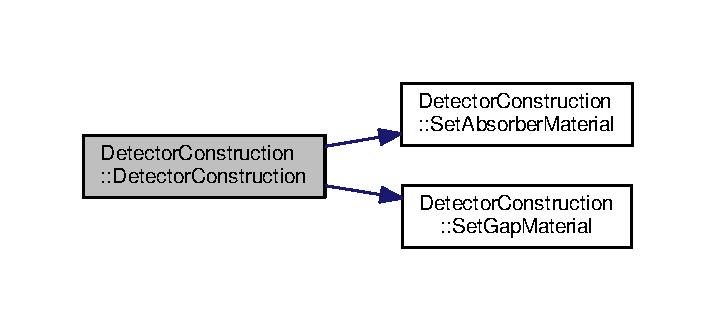
\includegraphics[width=344pt]{class_detector_construction_a1533c4308baddd0b2dcdf40f61dea1ef_cgraph}
\end{center}
\end{figure}


\hypertarget{class_detector_construction_a73013cab35a2b470338da2e4686edea3}{\index{Detector\-Construction@{Detector\-Construction}!$\sim$\-Detector\-Construction@{$\sim$\-Detector\-Construction}}
\index{$\sim$\-Detector\-Construction@{$\sim$\-Detector\-Construction}!DetectorConstruction@{Detector\-Construction}}
\subsubsection[{$\sim$\-Detector\-Construction}]{\setlength{\rightskip}{0pt plus 5cm}Detector\-Construction\-::$\sim$\-Detector\-Construction (
\begin{DoxyParamCaption}
{}
\end{DoxyParamCaption}
)}}\label{class_detector_construction_a73013cab35a2b470338da2e4686edea3}


Definition at line 84 of file Detector\-Construction.\-cc.



\subsection{Member Function Documentation}
\hypertarget{class_detector_construction_a662c618480b345a747f014b845d5ffdf}{\index{Detector\-Construction@{Detector\-Construction}!Construct@{Construct}}
\index{Construct@{Construct}!DetectorConstruction@{Detector\-Construction}}
\subsubsection[{Construct}]{\setlength{\rightskip}{0pt plus 5cm}G4\-V\-Physical\-Volume $\ast$ Detector\-Construction\-::\-Construct (
\begin{DoxyParamCaption}
{}
\end{DoxyParamCaption}
)}}\label{class_detector_construction_a662c618480b345a747f014b845d5ffdf}


Definition at line 89 of file Detector\-Construction.\-cc.

\hypertarget{class_detector_construction_ad893a559f7b2b8319df6e81c4b29f764}{\index{Detector\-Construction@{Detector\-Construction}!Get\-Absorber@{Get\-Absorber}}
\index{Get\-Absorber@{Get\-Absorber}!DetectorConstruction@{Detector\-Construction}}
\subsubsection[{Get\-Absorber}]{\setlength{\rightskip}{0pt plus 5cm}const G4\-V\-Physical\-Volume$\ast$ Detector\-Construction\-::\-Get\-Absorber (
\begin{DoxyParamCaption}
{}
\end{DoxyParamCaption}
)\hspace{0.3cm}{\ttfamily [inline]}}}\label{class_detector_construction_ad893a559f7b2b8319df6e81c4b29f764}


Definition at line 93 of file Detector\-Construction.\-hh.

\hypertarget{class_detector_construction_aec146766fd21440aef4e52b03e9b1151}{\index{Detector\-Construction@{Detector\-Construction}!Get\-Absorber\-Material@{Get\-Absorber\-Material}}
\index{Get\-Absorber\-Material@{Get\-Absorber\-Material}!DetectorConstruction@{Detector\-Construction}}
\subsubsection[{Get\-Absorber\-Material}]{\setlength{\rightskip}{0pt plus 5cm}G4\-Material$\ast$ Detector\-Construction\-::\-Get\-Absorber\-Material (
\begin{DoxyParamCaption}
{}
\end{DoxyParamCaption}
)\hspace{0.3cm}{\ttfamily [inline]}}}\label{class_detector_construction_aec146766fd21440aef4e52b03e9b1151}


Definition at line 86 of file Detector\-Construction.\-hh.

\hypertarget{class_detector_construction_a7d3cce8b138380c178cab2065d2f02c5}{\index{Detector\-Construction@{Detector\-Construction}!Get\-Absorber\-Thickness@{Get\-Absorber\-Thickness}}
\index{Get\-Absorber\-Thickness@{Get\-Absorber\-Thickness}!DetectorConstruction@{Detector\-Construction}}
\subsubsection[{Get\-Absorber\-Thickness}]{\setlength{\rightskip}{0pt plus 5cm}G4double Detector\-Construction\-::\-Get\-Absorber\-Thickness (
\begin{DoxyParamCaption}
{}
\end{DoxyParamCaption}
)\hspace{0.3cm}{\ttfamily [inline]}}}\label{class_detector_construction_a7d3cce8b138380c178cab2065d2f02c5}


Definition at line 87 of file Detector\-Construction.\-hh.

\hypertarget{class_detector_construction_a4b4ad895c4474577545bed10dea24a4d}{\index{Detector\-Construction@{Detector\-Construction}!Get\-Calor\-Size\-Y\-Z@{Get\-Calor\-Size\-Y\-Z}}
\index{Get\-Calor\-Size\-Y\-Z@{Get\-Calor\-Size\-Y\-Z}!DetectorConstruction@{Detector\-Construction}}
\subsubsection[{Get\-Calor\-Size\-Y\-Z}]{\setlength{\rightskip}{0pt plus 5cm}G4double Detector\-Construction\-::\-Get\-Calor\-Size\-Y\-Z (
\begin{DoxyParamCaption}
{}
\end{DoxyParamCaption}
)\hspace{0.3cm}{\ttfamily [inline]}}}\label{class_detector_construction_a4b4ad895c4474577545bed10dea24a4d}


Definition at line 82 of file Detector\-Construction.\-hh.

\hypertarget{class_detector_construction_a9ed9cc2835f90b9c22b509afbc298775}{\index{Detector\-Construction@{Detector\-Construction}!Get\-Calor\-Thickness@{Get\-Calor\-Thickness}}
\index{Get\-Calor\-Thickness@{Get\-Calor\-Thickness}!DetectorConstruction@{Detector\-Construction}}
\subsubsection[{Get\-Calor\-Thickness}]{\setlength{\rightskip}{0pt plus 5cm}G4double Detector\-Construction\-::\-Get\-Calor\-Thickness (
\begin{DoxyParamCaption}
{}
\end{DoxyParamCaption}
)\hspace{0.3cm}{\ttfamily [inline]}}}\label{class_detector_construction_a9ed9cc2835f90b9c22b509afbc298775}


Definition at line 81 of file Detector\-Construction.\-hh.

\hypertarget{class_detector_construction_aeccad9335e5931ad8fe30182dc61860b}{\index{Detector\-Construction@{Detector\-Construction}!Get\-Gap@{Get\-Gap}}
\index{Get\-Gap@{Get\-Gap}!DetectorConstruction@{Detector\-Construction}}
\subsubsection[{Get\-Gap}]{\setlength{\rightskip}{0pt plus 5cm}const G4\-V\-Physical\-Volume$\ast$ Detector\-Construction\-::\-Get\-Gap (
\begin{DoxyParamCaption}
{}
\end{DoxyParamCaption}
)\hspace{0.3cm}{\ttfamily [inline]}}}\label{class_detector_construction_aeccad9335e5931ad8fe30182dc61860b}


Definition at line 94 of file Detector\-Construction.\-hh.

\hypertarget{class_detector_construction_aa85d1cf09a67505d561814dc06c0934f}{\index{Detector\-Construction@{Detector\-Construction}!Get\-Gap\-Material@{Get\-Gap\-Material}}
\index{Get\-Gap\-Material@{Get\-Gap\-Material}!DetectorConstruction@{Detector\-Construction}}
\subsubsection[{Get\-Gap\-Material}]{\setlength{\rightskip}{0pt plus 5cm}G4\-Material$\ast$ Detector\-Construction\-::\-Get\-Gap\-Material (
\begin{DoxyParamCaption}
{}
\end{DoxyParamCaption}
)\hspace{0.3cm}{\ttfamily [inline]}}}\label{class_detector_construction_aa85d1cf09a67505d561814dc06c0934f}


Definition at line 89 of file Detector\-Construction.\-hh.

\hypertarget{class_detector_construction_ac0ec9c5c2273b936d68da16ef8efeda9}{\index{Detector\-Construction@{Detector\-Construction}!Get\-Gap\-Thickness@{Get\-Gap\-Thickness}}
\index{Get\-Gap\-Thickness@{Get\-Gap\-Thickness}!DetectorConstruction@{Detector\-Construction}}
\subsubsection[{Get\-Gap\-Thickness}]{\setlength{\rightskip}{0pt plus 5cm}G4double Detector\-Construction\-::\-Get\-Gap\-Thickness (
\begin{DoxyParamCaption}
{}
\end{DoxyParamCaption}
)\hspace{0.3cm}{\ttfamily [inline]}}}\label{class_detector_construction_ac0ec9c5c2273b936d68da16ef8efeda9}


Definition at line 90 of file Detector\-Construction.\-hh.

\hypertarget{class_detector_construction_a5b3b5f7a167a60774b2907181f4ead69}{\index{Detector\-Construction@{Detector\-Construction}!Get\-Nb\-Of\-Layers@{Get\-Nb\-Of\-Layers}}
\index{Get\-Nb\-Of\-Layers@{Get\-Nb\-Of\-Layers}!DetectorConstruction@{Detector\-Construction}}
\subsubsection[{Get\-Nb\-Of\-Layers}]{\setlength{\rightskip}{0pt plus 5cm}G4int Detector\-Construction\-::\-Get\-Nb\-Of\-Layers (
\begin{DoxyParamCaption}
{}
\end{DoxyParamCaption}
)\hspace{0.3cm}{\ttfamily [inline]}}}\label{class_detector_construction_a5b3b5f7a167a60774b2907181f4ead69}


Definition at line 84 of file Detector\-Construction.\-hh.

\hypertarget{class_detector_construction_a7ac14b0a6550779fe6ec481d13730f37}{\index{Detector\-Construction@{Detector\-Construction}!Getphysi\-World@{Getphysi\-World}}
\index{Getphysi\-World@{Getphysi\-World}!DetectorConstruction@{Detector\-Construction}}
\subsubsection[{Getphysi\-World}]{\setlength{\rightskip}{0pt plus 5cm}const G4\-V\-Physical\-Volume$\ast$ Detector\-Construction\-::\-Getphysi\-World (
\begin{DoxyParamCaption}
{}
\end{DoxyParamCaption}
)\hspace{0.3cm}{\ttfamily [inline]}}}\label{class_detector_construction_a7ac14b0a6550779fe6ec481d13730f37}


Definition at line 92 of file Detector\-Construction.\-hh.

\hypertarget{class_detector_construction_a08c8ac2151ce1dd90d46f14f74377276}{\index{Detector\-Construction@{Detector\-Construction}!Get\-World\-Size\-X@{Get\-World\-Size\-X}}
\index{Get\-World\-Size\-X@{Get\-World\-Size\-X}!DetectorConstruction@{Detector\-Construction}}
\subsubsection[{Get\-World\-Size\-X}]{\setlength{\rightskip}{0pt plus 5cm}G4double Detector\-Construction\-::\-Get\-World\-Size\-X (
\begin{DoxyParamCaption}
{}
\end{DoxyParamCaption}
)\hspace{0.3cm}{\ttfamily [inline]}}}\label{class_detector_construction_a08c8ac2151ce1dd90d46f14f74377276}


Definition at line 78 of file Detector\-Construction.\-hh.

\hypertarget{class_detector_construction_a2179692a66c262ebfdbf86f122264ff6}{\index{Detector\-Construction@{Detector\-Construction}!Get\-World\-Size\-Y\-Z@{Get\-World\-Size\-Y\-Z}}
\index{Get\-World\-Size\-Y\-Z@{Get\-World\-Size\-Y\-Z}!DetectorConstruction@{Detector\-Construction}}
\subsubsection[{Get\-World\-Size\-Y\-Z}]{\setlength{\rightskip}{0pt plus 5cm}G4double Detector\-Construction\-::\-Get\-World\-Size\-Y\-Z (
\begin{DoxyParamCaption}
{}
\end{DoxyParamCaption}
)\hspace{0.3cm}{\ttfamily [inline]}}}\label{class_detector_construction_a2179692a66c262ebfdbf86f122264ff6}


Definition at line 79 of file Detector\-Construction.\-hh.

\hypertarget{class_detector_construction_a47a2dfb018c7250eb1257bed265cab05}{\index{Detector\-Construction@{Detector\-Construction}!Print\-Calor\-Parameters@{Print\-Calor\-Parameters}}
\index{Print\-Calor\-Parameters@{Print\-Calor\-Parameters}!DetectorConstruction@{Detector\-Construction}}
\subsubsection[{Print\-Calor\-Parameters}]{\setlength{\rightskip}{0pt plus 5cm}void Detector\-Construction\-::\-Print\-Calor\-Parameters (
\begin{DoxyParamCaption}
{}
\end{DoxyParamCaption}
)}}\label{class_detector_construction_a47a2dfb018c7250eb1257bed265cab05}


Definition at line 392 of file Detector\-Construction.\-cc.

\hypertarget{class_detector_construction_a9b970ad4aacc014e624cc19ff5664d55}{\index{Detector\-Construction@{Detector\-Construction}!Set\-Absorber\-Material@{Set\-Absorber\-Material}}
\index{Set\-Absorber\-Material@{Set\-Absorber\-Material}!DetectorConstruction@{Detector\-Construction}}
\subsubsection[{Set\-Absorber\-Material}]{\setlength{\rightskip}{0pt plus 5cm}void Detector\-Construction\-::\-Set\-Absorber\-Material (
\begin{DoxyParamCaption}
\item[{G4\-String}]{material\-Choice}
\end{DoxyParamCaption}
)}}\label{class_detector_construction_a9b970ad4aacc014e624cc19ff5664d55}


Definition at line 404 of file Detector\-Construction.\-cc.



Here is the caller graph for this function\-:\nopagebreak
\begin{figure}[H]
\begin{center}
\leavevmode
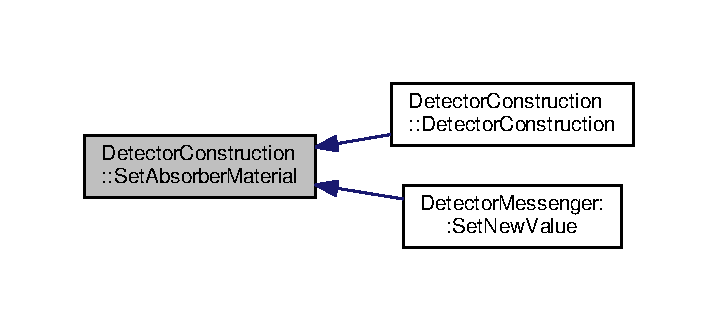
\includegraphics[width=344pt]{class_detector_construction_a9b970ad4aacc014e624cc19ff5664d55_icgraph}
\end{center}
\end{figure}


\hypertarget{class_detector_construction_a966fd78fdccca049843b5763246d594b}{\index{Detector\-Construction@{Detector\-Construction}!Set\-Absorber\-Thickness@{Set\-Absorber\-Thickness}}
\index{Set\-Absorber\-Thickness@{Set\-Absorber\-Thickness}!DetectorConstruction@{Detector\-Construction}}
\subsubsection[{Set\-Absorber\-Thickness}]{\setlength{\rightskip}{0pt plus 5cm}void Detector\-Construction\-::\-Set\-Absorber\-Thickness (
\begin{DoxyParamCaption}
\item[{G4double}]{val}
\end{DoxyParamCaption}
)}}\label{class_detector_construction_a966fd78fdccca049843b5763246d594b}


Definition at line 422 of file Detector\-Construction.\-cc.



Here is the caller graph for this function\-:\nopagebreak
\begin{figure}[H]
\begin{center}
\leavevmode
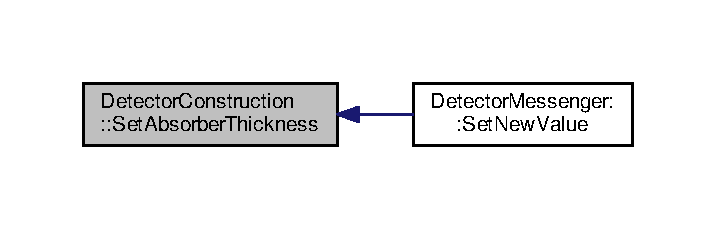
\includegraphics[width=344pt]{class_detector_construction_a966fd78fdccca049843b5763246d594b_icgraph}
\end{center}
\end{figure}


\hypertarget{class_detector_construction_a4e839c8ca5bdf75483333d32fe7912f4}{\index{Detector\-Construction@{Detector\-Construction}!Set\-Calor\-Size\-Y\-Z@{Set\-Calor\-Size\-Y\-Z}}
\index{Set\-Calor\-Size\-Y\-Z@{Set\-Calor\-Size\-Y\-Z}!DetectorConstruction@{Detector\-Construction}}
\subsubsection[{Set\-Calor\-Size\-Y\-Z}]{\setlength{\rightskip}{0pt plus 5cm}void Detector\-Construction\-::\-Set\-Calor\-Size\-Y\-Z (
\begin{DoxyParamCaption}
\item[{G4double}]{val}
\end{DoxyParamCaption}
)}}\label{class_detector_construction_a4e839c8ca5bdf75483333d32fe7912f4}


Definition at line 438 of file Detector\-Construction.\-cc.



Here is the caller graph for this function\-:\nopagebreak
\begin{figure}[H]
\begin{center}
\leavevmode
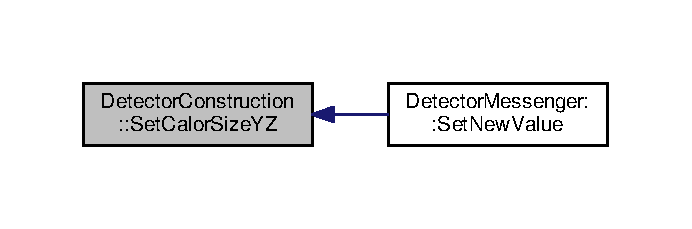
\includegraphics[width=332pt]{class_detector_construction_a4e839c8ca5bdf75483333d32fe7912f4_icgraph}
\end{center}
\end{figure}


\hypertarget{class_detector_construction_ae511a5f00b0f6b52b258426d981440cd}{\index{Detector\-Construction@{Detector\-Construction}!Set\-Gap\-Material@{Set\-Gap\-Material}}
\index{Set\-Gap\-Material@{Set\-Gap\-Material}!DetectorConstruction@{Detector\-Construction}}
\subsubsection[{Set\-Gap\-Material}]{\setlength{\rightskip}{0pt plus 5cm}void Detector\-Construction\-::\-Set\-Gap\-Material (
\begin{DoxyParamCaption}
\item[{G4\-String}]{material\-Choice}
\end{DoxyParamCaption}
)}}\label{class_detector_construction_ae511a5f00b0f6b52b258426d981440cd}


Definition at line 413 of file Detector\-Construction.\-cc.



Here is the caller graph for this function\-:\nopagebreak
\begin{figure}[H]
\begin{center}
\leavevmode
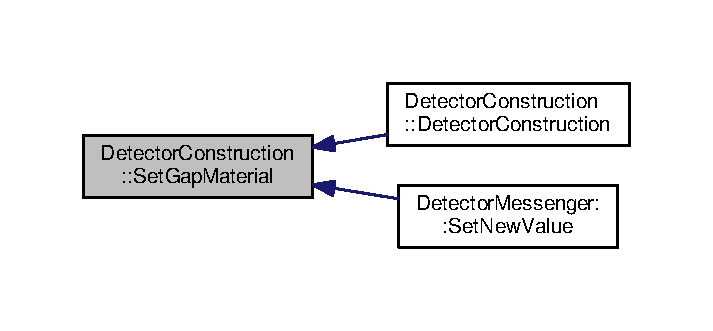
\includegraphics[width=342pt]{class_detector_construction_ae511a5f00b0f6b52b258426d981440cd_icgraph}
\end{center}
\end{figure}


\hypertarget{class_detector_construction_aa4fe52c7824b4272c9d6fdc54b906a4a}{\index{Detector\-Construction@{Detector\-Construction}!Set\-Gap\-Thickness@{Set\-Gap\-Thickness}}
\index{Set\-Gap\-Thickness@{Set\-Gap\-Thickness}!DetectorConstruction@{Detector\-Construction}}
\subsubsection[{Set\-Gap\-Thickness}]{\setlength{\rightskip}{0pt plus 5cm}void Detector\-Construction\-::\-Set\-Gap\-Thickness (
\begin{DoxyParamCaption}
\item[{G4double}]{val}
\end{DoxyParamCaption}
)}}\label{class_detector_construction_aa4fe52c7824b4272c9d6fdc54b906a4a}


Definition at line 430 of file Detector\-Construction.\-cc.



Here is the caller graph for this function\-:\nopagebreak
\begin{figure}[H]
\begin{center}
\leavevmode
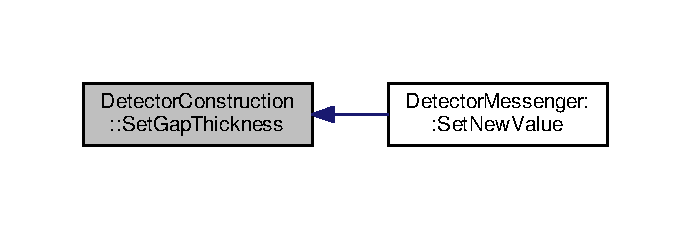
\includegraphics[width=332pt]{class_detector_construction_aa4fe52c7824b4272c9d6fdc54b906a4a_icgraph}
\end{center}
\end{figure}


\hypertarget{class_detector_construction_a63ab08aef61c63c09b59019e4d586d60}{\index{Detector\-Construction@{Detector\-Construction}!Set\-Mag\-Field@{Set\-Mag\-Field}}
\index{Set\-Mag\-Field@{Set\-Mag\-Field}!DetectorConstruction@{Detector\-Construction}}
\subsubsection[{Set\-Mag\-Field}]{\setlength{\rightskip}{0pt plus 5cm}void Detector\-Construction\-::\-Set\-Mag\-Field (
\begin{DoxyParamCaption}
\item[{G4double}]{field\-Value}
\end{DoxyParamCaption}
)}}\label{class_detector_construction_a63ab08aef61c63c09b59019e4d586d60}


Definition at line 456 of file Detector\-Construction.\-cc.



Here is the caller graph for this function\-:\nopagebreak
\begin{figure}[H]
\begin{center}
\leavevmode
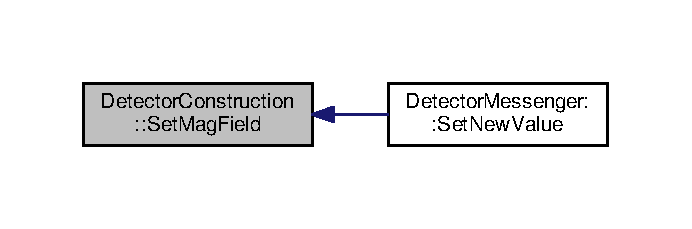
\includegraphics[width=332pt]{class_detector_construction_a63ab08aef61c63c09b59019e4d586d60_icgraph}
\end{center}
\end{figure}


\hypertarget{class_detector_construction_a9c0e7bcf321ffb2c6c3b6e51aa79a9f7}{\index{Detector\-Construction@{Detector\-Construction}!Set\-Nb\-Of\-Layers@{Set\-Nb\-Of\-Layers}}
\index{Set\-Nb\-Of\-Layers@{Set\-Nb\-Of\-Layers}!DetectorConstruction@{Detector\-Construction}}
\subsubsection[{Set\-Nb\-Of\-Layers}]{\setlength{\rightskip}{0pt plus 5cm}void Detector\-Construction\-::\-Set\-Nb\-Of\-Layers (
\begin{DoxyParamCaption}
\item[{G4int}]{val}
\end{DoxyParamCaption}
)}}\label{class_detector_construction_a9c0e7bcf321ffb2c6c3b6e51aa79a9f7}


Definition at line 446 of file Detector\-Construction.\-cc.



Here is the caller graph for this function\-:\nopagebreak
\begin{figure}[H]
\begin{center}
\leavevmode
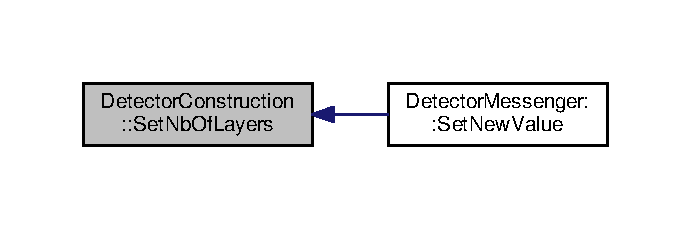
\includegraphics[width=332pt]{class_detector_construction_a9c0e7bcf321ffb2c6c3b6e51aa79a9f7_icgraph}
\end{center}
\end{figure}


\hypertarget{class_detector_construction_a2742ef0ae83433992902a56693f2c6e5}{\index{Detector\-Construction@{Detector\-Construction}!Update\-Geometry@{Update\-Geometry}}
\index{Update\-Geometry@{Update\-Geometry}!DetectorConstruction@{Detector\-Construction}}
\subsubsection[{Update\-Geometry}]{\setlength{\rightskip}{0pt plus 5cm}void Detector\-Construction\-::\-Update\-Geometry (
\begin{DoxyParamCaption}
{}
\end{DoxyParamCaption}
)}}\label{class_detector_construction_a2742ef0ae83433992902a56693f2c6e5}


Definition at line 478 of file Detector\-Construction.\-cc.



Here is the caller graph for this function\-:\nopagebreak
\begin{figure}[H]
\begin{center}
\leavevmode
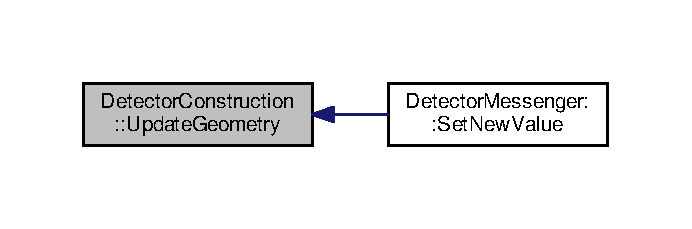
\includegraphics[width=332pt]{class_detector_construction_a2742ef0ae83433992902a56693f2c6e5_icgraph}
\end{center}
\end{figure}




The documentation for this class was generated from the following files\-:\begin{DoxyCompactItemize}
\item 
g4work/\-Ecal/include/\hyperlink{_detector_construction_8hh}{Detector\-Construction.\-hh}\item 
g4work/\-Ecal/src/\hyperlink{_detector_construction_8cc}{Detector\-Construction.\-cc}\end{DoxyCompactItemize}

\hypertarget{class_detector_messenger}{\section{Detector\-Messenger Class Reference}
\label{class_detector_messenger}\index{Detector\-Messenger@{Detector\-Messenger}}
}


{\ttfamily \#include $<$Detector\-Messenger.\-hh$>$}

\subsection*{Public Member Functions}
\begin{DoxyCompactItemize}
\item 
\hyperlink{class_detector_messenger_a53c8ae094fc5dc843cd7944f03e663d0}{Detector\-Messenger} (\hyperlink{class_detector_construction}{Detector\-Construction} $\ast$)
\item 
\hyperlink{class_detector_messenger_a2a68551db9aa6fb18ec533d6ff7c7d12}{$\sim$\-Detector\-Messenger} ()
\item 
void \hyperlink{class_detector_messenger_a855728d4ce6ae4397282bc7375740f2b}{Set\-New\-Value} (G4\-U\-Icommand $\ast$, G4\-String)
\end{DoxyCompactItemize}


\subsection{Detailed Description}


Definition at line 50 of file Detector\-Messenger.\-hh.



\subsection{Constructor \& Destructor Documentation}
\hypertarget{class_detector_messenger_a53c8ae094fc5dc843cd7944f03e663d0}{\index{Detector\-Messenger@{Detector\-Messenger}!Detector\-Messenger@{Detector\-Messenger}}
\index{Detector\-Messenger@{Detector\-Messenger}!DetectorMessenger@{Detector\-Messenger}}
\subsubsection[{Detector\-Messenger}]{\setlength{\rightskip}{0pt plus 5cm}Detector\-Messenger\-::\-Detector\-Messenger (
\begin{DoxyParamCaption}
\item[{{\bf Detector\-Construction} $\ast$}]{Det}
\end{DoxyParamCaption}
)}}\label{class_detector_messenger_a53c8ae094fc5dc843cd7944f03e663d0}


Definition at line 46 of file Detector\-Messenger.\-cc.

\hypertarget{class_detector_messenger_a2a68551db9aa6fb18ec533d6ff7c7d12}{\index{Detector\-Messenger@{Detector\-Messenger}!$\sim$\-Detector\-Messenger@{$\sim$\-Detector\-Messenger}}
\index{$\sim$\-Detector\-Messenger@{$\sim$\-Detector\-Messenger}!DetectorMessenger@{Detector\-Messenger}}
\subsubsection[{$\sim$\-Detector\-Messenger}]{\setlength{\rightskip}{0pt plus 5cm}Detector\-Messenger\-::$\sim$\-Detector\-Messenger (
\begin{DoxyParamCaption}
{}
\end{DoxyParamCaption}
)}}\label{class_detector_messenger_a2a68551db9aa6fb18ec533d6ff7c7d12}


Definition at line 109 of file Detector\-Messenger.\-cc.



\subsection{Member Function Documentation}
\hypertarget{class_detector_messenger_a855728d4ce6ae4397282bc7375740f2b}{\index{Detector\-Messenger@{Detector\-Messenger}!Set\-New\-Value@{Set\-New\-Value}}
\index{Set\-New\-Value@{Set\-New\-Value}!DetectorMessenger@{Detector\-Messenger}}
\subsubsection[{Set\-New\-Value}]{\setlength{\rightskip}{0pt plus 5cm}void Detector\-Messenger\-::\-Set\-New\-Value (
\begin{DoxyParamCaption}
\item[{G4\-U\-Icommand $\ast$}]{command, }
\item[{G4\-String}]{new\-Value}
\end{DoxyParamCaption}
)}}\label{class_detector_messenger_a855728d4ce6ae4397282bc7375740f2b}


Definition at line 122 of file Detector\-Messenger.\-cc.



Here is the call graph for this function\-:\nopagebreak
\begin{figure}[H]
\begin{center}
\leavevmode
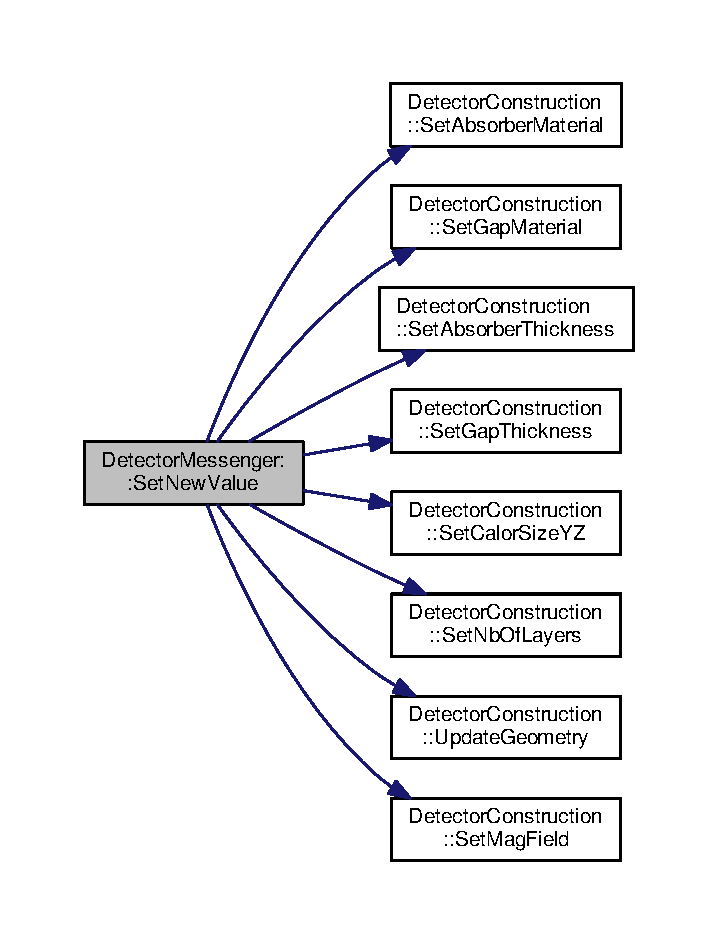
\includegraphics[width=344pt]{class_detector_messenger_a855728d4ce6ae4397282bc7375740f2b_cgraph}
\end{center}
\end{figure}




The documentation for this class was generated from the following files\-:\begin{DoxyCompactItemize}
\item 
g4work/\-Ecal/include/\hyperlink{_detector_messenger_8hh}{Detector\-Messenger.\-hh}\item 
g4work/\-Ecal/src/\hyperlink{_detector_messenger_8cc}{Detector\-Messenger.\-cc}\end{DoxyCompactItemize}

\hypertarget{class_e_cal_analysis}{\section{E\-Cal\-Analysis Class Reference}
\label{class_e_cal_analysis}\index{E\-Cal\-Analysis@{E\-Cal\-Analysis}}
}


{\ttfamily \#include $<$E\-Cal\-Analysis.\-hh$>$}

\subsection*{Public Member Functions}
\begin{DoxyCompactItemize}
\item 
\hyperlink{class_e_cal_analysis_ac36fe71ad15447afcd56596132402037}{E\-Cal\-Analysis} ()
\item 
\hyperlink{class_e_cal_analysis_a9f14afb8f9e07b0f618507c4cdd5c561}{$\sim$\-E\-Cal\-Analysis} ()
\item 
void \hyperlink{class_e_cal_analysis_ac4e972975d457daed4d984a5fce70b90}{Begin\-Of\-Run\-Action} (const G4\-Run $\ast$)
\item 
void \hyperlink{class_e_cal_analysis_abb9d6687444b46ae43647137eb72e0e2}{End\-Of\-Run\-Action} (const G4\-Run $\ast$)
\item 
void \hyperlink{class_e_cal_analysis_adbc751b8a7b0d09714f3d98039e057ba}{Begin\-Of\-Event\-Action} (const G4\-Event $\ast$)
\item 
void \hyperlink{class_e_cal_analysis_a2b22c032753423855ca8af965f2c5f0d}{End\-Of\-Event\-Action} (const G4\-Event $\ast$)
\item 
void \hyperlink{class_e_cal_analysis_a767674ded7fc8a46699d12f6eb7be80f}{Track\-Start\-Action} ()
\item 
void \hyperlink{class_e_cal_analysis_ab51cb6fd622be54138d98c8e72d0add4}{Track\-Stop\-Action} ()
\item 
void \hyperlink{class_e_cal_analysis_a8e9d71768cb60d23faecd6b75b88c060}{Step\-Aceptance} (const G4\-Step $\ast$a\-Step)
\item 
void \hyperlink{class_e_cal_analysis_aa9f1dd2a2863ed234a030f75b2171989}{dosave} ()
\end{DoxyCompactItemize}


\subsection{Detailed Description}


Definition at line 71 of file E\-Cal\-Analysis.\-hh.



\subsection{Constructor \& Destructor Documentation}
\hypertarget{class_e_cal_analysis_ac36fe71ad15447afcd56596132402037}{\index{E\-Cal\-Analysis@{E\-Cal\-Analysis}!E\-Cal\-Analysis@{E\-Cal\-Analysis}}
\index{E\-Cal\-Analysis@{E\-Cal\-Analysis}!ECalAnalysis@{E\-Cal\-Analysis}}
\subsubsection[{E\-Cal\-Analysis}]{\setlength{\rightskip}{0pt plus 5cm}E\-Cal\-Analysis\-::\-E\-Cal\-Analysis (
\begin{DoxyParamCaption}
{}
\end{DoxyParamCaption}
)}}\label{class_e_cal_analysis_ac36fe71ad15447afcd56596132402037}


Definition at line 42 of file E\-Cal\-Analysis.\-cc.

\hypertarget{class_e_cal_analysis_a9f14afb8f9e07b0f618507c4cdd5c561}{\index{E\-Cal\-Analysis@{E\-Cal\-Analysis}!$\sim$\-E\-Cal\-Analysis@{$\sim$\-E\-Cal\-Analysis}}
\index{$\sim$\-E\-Cal\-Analysis@{$\sim$\-E\-Cal\-Analysis}!ECalAnalysis@{E\-Cal\-Analysis}}
\subsubsection[{$\sim$\-E\-Cal\-Analysis}]{\setlength{\rightskip}{0pt plus 5cm}E\-Cal\-Analysis\-::$\sim$\-E\-Cal\-Analysis (
\begin{DoxyParamCaption}
{}
\end{DoxyParamCaption}
)}}\label{class_e_cal_analysis_a9f14afb8f9e07b0f618507c4cdd5c561}


Definition at line 53 of file E\-Cal\-Analysis.\-cc.



\subsection{Member Function Documentation}
\hypertarget{class_e_cal_analysis_adbc751b8a7b0d09714f3d98039e057ba}{\index{E\-Cal\-Analysis@{E\-Cal\-Analysis}!Begin\-Of\-Event\-Action@{Begin\-Of\-Event\-Action}}
\index{Begin\-Of\-Event\-Action@{Begin\-Of\-Event\-Action}!ECalAnalysis@{E\-Cal\-Analysis}}
\subsubsection[{Begin\-Of\-Event\-Action}]{\setlength{\rightskip}{0pt plus 5cm}void E\-Cal\-Analysis\-::\-Begin\-Of\-Event\-Action (
\begin{DoxyParamCaption}
\item[{const G4\-Event $\ast$}]{an\-Event}
\end{DoxyParamCaption}
)}}\label{class_e_cal_analysis_adbc751b8a7b0d09714f3d98039e057ba}


Definition at line 161 of file E\-Cal\-Analysis.\-cc.



Here is the caller graph for this function\-:\nopagebreak
\begin{figure}[H]
\begin{center}
\leavevmode
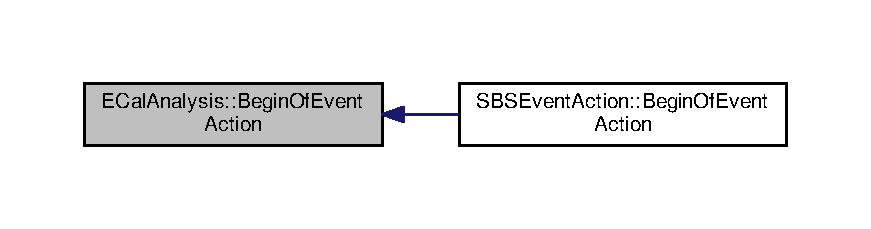
\includegraphics[width=350pt]{class_e_cal_analysis_adbc751b8a7b0d09714f3d98039e057ba_icgraph}
\end{center}
\end{figure}


\hypertarget{class_e_cal_analysis_ac4e972975d457daed4d984a5fce70b90}{\index{E\-Cal\-Analysis@{E\-Cal\-Analysis}!Begin\-Of\-Run\-Action@{Begin\-Of\-Run\-Action}}
\index{Begin\-Of\-Run\-Action@{Begin\-Of\-Run\-Action}!ECalAnalysis@{E\-Cal\-Analysis}}
\subsubsection[{Begin\-Of\-Run\-Action}]{\setlength{\rightskip}{0pt plus 5cm}void E\-Cal\-Analysis\-::\-Begin\-Of\-Run\-Action (
\begin{DoxyParamCaption}
\item[{const G4\-Run $\ast$}]{a\-Run}
\end{DoxyParamCaption}
)}}\label{class_e_cal_analysis_ac4e972975d457daed4d984a5fce70b90}


Definition at line 67 of file E\-Cal\-Analysis.\-cc.



Here is the caller graph for this function\-:\nopagebreak
\begin{figure}[H]
\begin{center}
\leavevmode
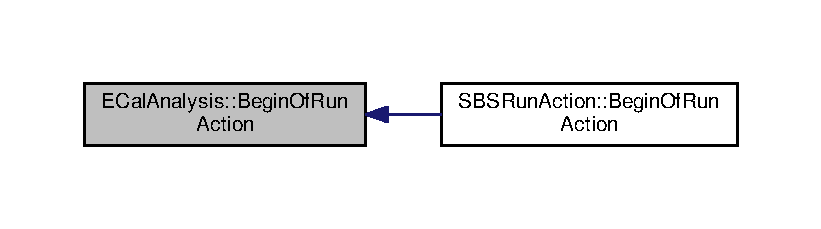
\includegraphics[width=350pt]{class_e_cal_analysis_ac4e972975d457daed4d984a5fce70b90_icgraph}
\end{center}
\end{figure}


\hypertarget{class_e_cal_analysis_aa9f1dd2a2863ed234a030f75b2171989}{\index{E\-Cal\-Analysis@{E\-Cal\-Analysis}!dosave@{dosave}}
\index{dosave@{dosave}!ECalAnalysis@{E\-Cal\-Analysis}}
\subsubsection[{dosave}]{\setlength{\rightskip}{0pt plus 5cm}void E\-Cal\-Analysis\-::dosave (
\begin{DoxyParamCaption}
{}
\end{DoxyParamCaption}
)}}\label{class_e_cal_analysis_aa9f1dd2a2863ed234a030f75b2171989}


Definition at line 487 of file E\-Cal\-Analysis.\-cc.



Here is the caller graph for this function\-:
\nopagebreak
\begin{figure}[H]
\begin{center}
\leavevmode
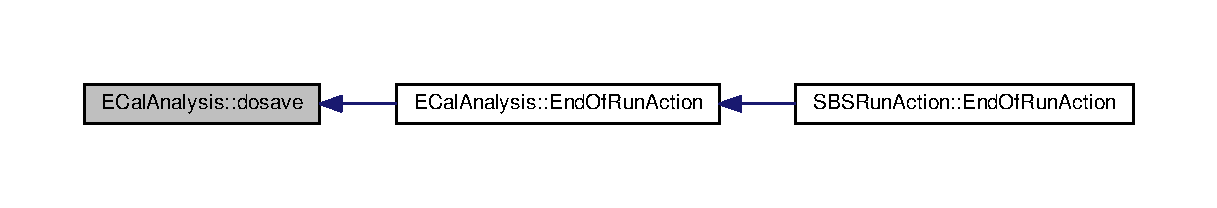
\includegraphics[width=350pt]{class_e_cal_analysis_aa9f1dd2a2863ed234a030f75b2171989_icgraph}
\end{center}
\end{figure}


\hypertarget{class_e_cal_analysis_a2b22c032753423855ca8af965f2c5f0d}{\index{E\-Cal\-Analysis@{E\-Cal\-Analysis}!End\-Of\-Event\-Action@{End\-Of\-Event\-Action}}
\index{End\-Of\-Event\-Action@{End\-Of\-Event\-Action}!ECalAnalysis@{E\-Cal\-Analysis}}
\subsubsection[{End\-Of\-Event\-Action}]{\setlength{\rightskip}{0pt plus 5cm}void E\-Cal\-Analysis\-::\-End\-Of\-Event\-Action (
\begin{DoxyParamCaption}
\item[{const G4\-Event $\ast$}]{an\-Event}
\end{DoxyParamCaption}
)}}\label{class_e_cal_analysis_a2b22c032753423855ca8af965f2c5f0d}


Definition at line 214 of file E\-Cal\-Analysis.\-cc.



Here is the caller graph for this function\-:\nopagebreak
\begin{figure}[H]
\begin{center}
\leavevmode
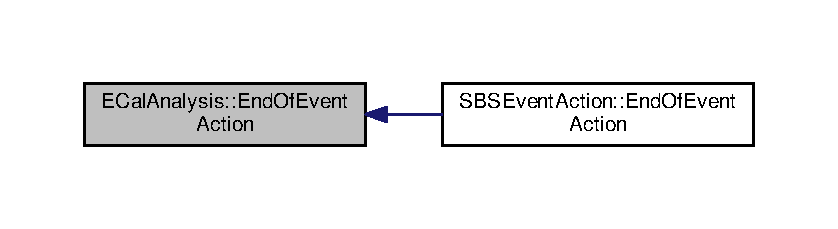
\includegraphics[width=350pt]{class_e_cal_analysis_a2b22c032753423855ca8af965f2c5f0d_icgraph}
\end{center}
\end{figure}


\hypertarget{class_e_cal_analysis_abb9d6687444b46ae43647137eb72e0e2}{\index{E\-Cal\-Analysis@{E\-Cal\-Analysis}!End\-Of\-Run\-Action@{End\-Of\-Run\-Action}}
\index{End\-Of\-Run\-Action@{End\-Of\-Run\-Action}!ECalAnalysis@{E\-Cal\-Analysis}}
\subsubsection[{End\-Of\-Run\-Action}]{\setlength{\rightskip}{0pt plus 5cm}void E\-Cal\-Analysis\-::\-End\-Of\-Run\-Action (
\begin{DoxyParamCaption}
\item[{const G4\-Run $\ast$}]{a\-Run}
\end{DoxyParamCaption}
)}}\label{class_e_cal_analysis_abb9d6687444b46ae43647137eb72e0e2}


Definition at line 97 of file E\-Cal\-Analysis.\-cc.



Here is the call graph for this function\-:\nopagebreak
\begin{figure}[H]
\begin{center}
\leavevmode
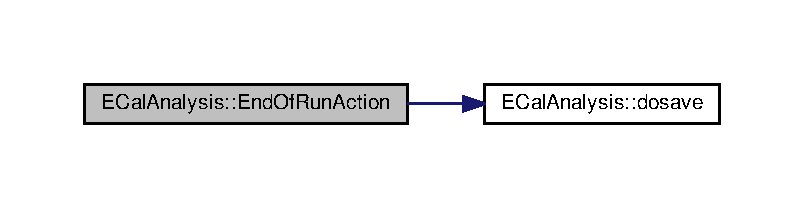
\includegraphics[width=350pt]{class_e_cal_analysis_abb9d6687444b46ae43647137eb72e0e2_cgraph}
\end{center}
\end{figure}




Here is the caller graph for this function\-:
\nopagebreak
\begin{figure}[H]
\begin{center}
\leavevmode
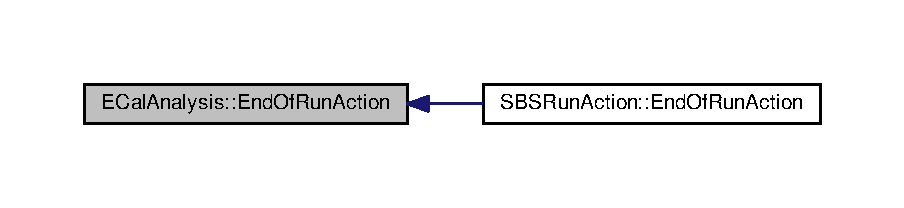
\includegraphics[width=350pt]{class_e_cal_analysis_abb9d6687444b46ae43647137eb72e0e2_icgraph}
\end{center}
\end{figure}


\hypertarget{class_e_cal_analysis_a8e9d71768cb60d23faecd6b75b88c060}{\index{E\-Cal\-Analysis@{E\-Cal\-Analysis}!Step\-Aceptance@{Step\-Aceptance}}
\index{Step\-Aceptance@{Step\-Aceptance}!ECalAnalysis@{E\-Cal\-Analysis}}
\subsubsection[{Step\-Aceptance}]{\setlength{\rightskip}{0pt plus 5cm}void E\-Cal\-Analysis\-::\-Step\-Aceptance (
\begin{DoxyParamCaption}
\item[{const G4\-Step $\ast$}]{a\-Step}
\end{DoxyParamCaption}
)}}\label{class_e_cal_analysis_a8e9d71768cb60d23faecd6b75b88c060}


Definition at line 366 of file E\-Cal\-Analysis.\-cc.



Here is the caller graph for this function\-:\nopagebreak
\begin{figure}[H]
\begin{center}
\leavevmode
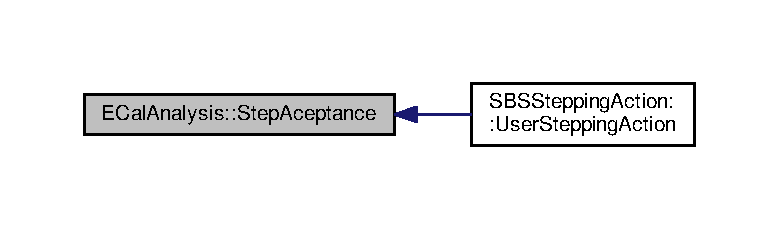
\includegraphics[width=350pt]{class_e_cal_analysis_a8e9d71768cb60d23faecd6b75b88c060_icgraph}
\end{center}
\end{figure}


\hypertarget{class_e_cal_analysis_a767674ded7fc8a46699d12f6eb7be80f}{\index{E\-Cal\-Analysis@{E\-Cal\-Analysis}!Track\-Start\-Action@{Track\-Start\-Action}}
\index{Track\-Start\-Action@{Track\-Start\-Action}!ECalAnalysis@{E\-Cal\-Analysis}}
\subsubsection[{Track\-Start\-Action}]{\setlength{\rightskip}{0pt plus 5cm}void E\-Cal\-Analysis\-::\-Track\-Start\-Action (
\begin{DoxyParamCaption}
{}
\end{DoxyParamCaption}
)}}\label{class_e_cal_analysis_a767674ded7fc8a46699d12f6eb7be80f}


Definition at line 315 of file E\-Cal\-Analysis.\-cc.

\hypertarget{class_e_cal_analysis_ab51cb6fd622be54138d98c8e72d0add4}{\index{E\-Cal\-Analysis@{E\-Cal\-Analysis}!Track\-Stop\-Action@{Track\-Stop\-Action}}
\index{Track\-Stop\-Action@{Track\-Stop\-Action}!ECalAnalysis@{E\-Cal\-Analysis}}
\subsubsection[{Track\-Stop\-Action}]{\setlength{\rightskip}{0pt plus 5cm}void E\-Cal\-Analysis\-::\-Track\-Stop\-Action (
\begin{DoxyParamCaption}
{}
\end{DoxyParamCaption}
)}}\label{class_e_cal_analysis_ab51cb6fd622be54138d98c8e72d0add4}


Definition at line 342 of file E\-Cal\-Analysis.\-cc.



The documentation for this class was generated from the following files\-:\begin{DoxyCompactItemize}
\item 
g4work/\-Ecal/include/\hyperlink{_e_cal_analysis_8hh}{E\-Cal\-Analysis.\-hh}\item 
g4work/\-Ecal/src/\hyperlink{_e_cal_analysis_8cc}{E\-Cal\-Analysis.\-cc}\end{DoxyCompactItemize}

\hypertarget{class_e_cal_detector_construction}{\section{E\-Cal\-Detector\-Construction Class Reference}
\label{class_e_cal_detector_construction}\index{E\-Cal\-Detector\-Construction@{E\-Cal\-Detector\-Construction}}
}


{\ttfamily \#include $<$E\-Cal\-Detector\-Construction.\-hh$>$}

\subsection*{Public Member Functions}
\begin{DoxyCompactItemize}
\item 
\hyperlink{class_e_cal_detector_construction_ad7b4dc31e1138aa6f3ee99b7b5bc60af}{E\-Cal\-Detector\-Construction} (G4\-V\-Physical\-Volume $\ast$physi\-Parent, \hyperlink{class_s_b_s_materials}{S\-B\-S\-Materials} $\ast$Materials)
\item 
\hyperlink{class_e_cal_detector_construction_a28e034fc3c3961369812c3e363719072}{$\sim$\-E\-Cal\-Detector\-Construction} ()
\item 
void \hyperlink{class_e_cal_detector_construction_aa1f9eb7928fee8e2dd62d488b60fc6f7}{Update\-Geometry} ()
\item 
G4\-V\-Physical\-Volume $\ast$ \hyperlink{class_e_cal_detector_construction_ac50bfcd7b4b64dc1a72cad91b131efb9}{Get\-Absorber} ()
\item 
G4\-V\-Physical\-Volume $\ast$ \hyperlink{class_e_cal_detector_construction_a97440bb92db785649209d6e3fbd84dd9}{Get\-Gap} ()
\end{DoxyCompactItemize}


\subsection{Detailed Description}


Definition at line 56 of file E\-Cal\-Detector\-Construction.\-hh.



\subsection{Constructor \& Destructor Documentation}
\hypertarget{class_e_cal_detector_construction_ad7b4dc31e1138aa6f3ee99b7b5bc60af}{\index{E\-Cal\-Detector\-Construction@{E\-Cal\-Detector\-Construction}!E\-Cal\-Detector\-Construction@{E\-Cal\-Detector\-Construction}}
\index{E\-Cal\-Detector\-Construction@{E\-Cal\-Detector\-Construction}!ECalDetectorConstruction@{E\-Cal\-Detector\-Construction}}
\subsubsection[{E\-Cal\-Detector\-Construction}]{\setlength{\rightskip}{0pt plus 5cm}E\-Cal\-Detector\-Construction\-::\-E\-Cal\-Detector\-Construction (
\begin{DoxyParamCaption}
\item[{G4\-V\-Physical\-Volume $\ast$}]{physi\-Parent, }
\item[{{\bf S\-B\-S\-Materials} $\ast$}]{Materials}
\end{DoxyParamCaption}
)}}\label{class_e_cal_detector_construction_ad7b4dc31e1138aa6f3ee99b7b5bc60af}


Definition at line 67 of file E\-Cal\-Detector\-Construction.\-cc.

\hypertarget{class_e_cal_detector_construction_a28e034fc3c3961369812c3e363719072}{\index{E\-Cal\-Detector\-Construction@{E\-Cal\-Detector\-Construction}!$\sim$\-E\-Cal\-Detector\-Construction@{$\sim$\-E\-Cal\-Detector\-Construction}}
\index{$\sim$\-E\-Cal\-Detector\-Construction@{$\sim$\-E\-Cal\-Detector\-Construction}!ECalDetectorConstruction@{E\-Cal\-Detector\-Construction}}
\subsubsection[{$\sim$\-E\-Cal\-Detector\-Construction}]{\setlength{\rightskip}{0pt plus 5cm}E\-Cal\-Detector\-Construction\-::$\sim$\-E\-Cal\-Detector\-Construction (
\begin{DoxyParamCaption}
{}
\end{DoxyParamCaption}
)}}\label{class_e_cal_detector_construction_a28e034fc3c3961369812c3e363719072}


Definition at line 481 of file E\-Cal\-Detector\-Construction.\-cc.



\subsection{Member Function Documentation}
\hypertarget{class_e_cal_detector_construction_ac50bfcd7b4b64dc1a72cad91b131efb9}{\index{E\-Cal\-Detector\-Construction@{E\-Cal\-Detector\-Construction}!Get\-Absorber@{Get\-Absorber}}
\index{Get\-Absorber@{Get\-Absorber}!ECalDetectorConstruction@{E\-Cal\-Detector\-Construction}}
\subsubsection[{Get\-Absorber}]{\setlength{\rightskip}{0pt plus 5cm}G4\-V\-Physical\-Volume$\ast$ E\-Cal\-Detector\-Construction\-::\-Get\-Absorber (
\begin{DoxyParamCaption}
{}
\end{DoxyParamCaption}
)\hspace{0.3cm}{\ttfamily [inline]}}}\label{class_e_cal_detector_construction_ac50bfcd7b4b64dc1a72cad91b131efb9}


Definition at line 70 of file E\-Cal\-Detector\-Construction.\-hh.

\hypertarget{class_e_cal_detector_construction_a97440bb92db785649209d6e3fbd84dd9}{\index{E\-Cal\-Detector\-Construction@{E\-Cal\-Detector\-Construction}!Get\-Gap@{Get\-Gap}}
\index{Get\-Gap@{Get\-Gap}!ECalDetectorConstruction@{E\-Cal\-Detector\-Construction}}
\subsubsection[{Get\-Gap}]{\setlength{\rightskip}{0pt plus 5cm}G4\-V\-Physical\-Volume$\ast$ E\-Cal\-Detector\-Construction\-::\-Get\-Gap (
\begin{DoxyParamCaption}
{}
\end{DoxyParamCaption}
)\hspace{0.3cm}{\ttfamily [inline]}}}\label{class_e_cal_detector_construction_a97440bb92db785649209d6e3fbd84dd9}


Definition at line 71 of file E\-Cal\-Detector\-Construction.\-hh.

\hypertarget{class_e_cal_detector_construction_aa1f9eb7928fee8e2dd62d488b60fc6f7}{\index{E\-Cal\-Detector\-Construction@{E\-Cal\-Detector\-Construction}!Update\-Geometry@{Update\-Geometry}}
\index{Update\-Geometry@{Update\-Geometry}!ECalDetectorConstruction@{E\-Cal\-Detector\-Construction}}
\subsubsection[{Update\-Geometry}]{\setlength{\rightskip}{0pt plus 5cm}void E\-Cal\-Detector\-Construction\-::\-Update\-Geometry (
\begin{DoxyParamCaption}
{}
\end{DoxyParamCaption}
)}}\label{class_e_cal_detector_construction_aa1f9eb7928fee8e2dd62d488b60fc6f7}


The documentation for this class was generated from the following files\-:\begin{DoxyCompactItemize}
\item 
g4work/\-Ecal/include/\hyperlink{_e_cal_detector_construction_8hh}{E\-Cal\-Detector\-Construction.\-hh}\item 
g4work/\-Ecal/src/\hyperlink{_e_cal_detector_construction_8cc}{E\-Cal\-Detector\-Construction.\-cc}\end{DoxyCompactItemize}

\hypertarget{class_event_action_messenger}{\section{Event\-Action\-Messenger Class Reference}
\label{class_event_action_messenger}\index{Event\-Action\-Messenger@{Event\-Action\-Messenger}}
}


{\ttfamily \#include $<$Event\-Action\-Messenger.\-hh$>$}

\subsection*{Public Member Functions}
\begin{DoxyCompactItemize}
\item 
\hyperlink{class_event_action_messenger_af386962abdd8df522f262a8083e5c0ab}{Event\-Action\-Messenger} (\hyperlink{class_s_b_s_event_action}{S\-B\-S\-Event\-Action} $\ast$)
\item 
virtual \hyperlink{class_event_action_messenger_afd0bc28f7304ab82a49912bfd8919fa8}{$\sim$\-Event\-Action\-Messenger} ()
\item 
void \hyperlink{class_event_action_messenger_a5e0f6b3ab8d2b596b195b71f1111f934}{Set\-New\-Value} (G4\-U\-Icommand $\ast$, G4\-String)
\end{DoxyCompactItemize}


\subsection{Detailed Description}


Definition at line 47 of file Event\-Action\-Messenger.\-hh.



\subsection{Constructor \& Destructor Documentation}
\hypertarget{class_event_action_messenger_af386962abdd8df522f262a8083e5c0ab}{\index{Event\-Action\-Messenger@{Event\-Action\-Messenger}!Event\-Action\-Messenger@{Event\-Action\-Messenger}}
\index{Event\-Action\-Messenger@{Event\-Action\-Messenger}!EventActionMessenger@{Event\-Action\-Messenger}}
\subsubsection[{Event\-Action\-Messenger}]{\setlength{\rightskip}{0pt plus 5cm}Event\-Action\-Messenger\-::\-Event\-Action\-Messenger (
\begin{DoxyParamCaption}
\item[{{\bf S\-B\-S\-Event\-Action} $\ast$}]{Ev\-Act}
\end{DoxyParamCaption}
)}}\label{class_event_action_messenger_af386962abdd8df522f262a8083e5c0ab}


Definition at line 44 of file Event\-Action\-Messenger.\-cc.

\hypertarget{class_event_action_messenger_afd0bc28f7304ab82a49912bfd8919fa8}{\index{Event\-Action\-Messenger@{Event\-Action\-Messenger}!$\sim$\-Event\-Action\-Messenger@{$\sim$\-Event\-Action\-Messenger}}
\index{$\sim$\-Event\-Action\-Messenger@{$\sim$\-Event\-Action\-Messenger}!EventActionMessenger@{Event\-Action\-Messenger}}
\subsubsection[{$\sim$\-Event\-Action\-Messenger}]{\setlength{\rightskip}{0pt plus 5cm}Event\-Action\-Messenger\-::$\sim$\-Event\-Action\-Messenger (
\begin{DoxyParamCaption}
{}
\end{DoxyParamCaption}
)\hspace{0.3cm}{\ttfamily [virtual]}}}\label{class_event_action_messenger_afd0bc28f7304ab82a49912bfd8919fa8}


Definition at line 58 of file Event\-Action\-Messenger.\-cc.



\subsection{Member Function Documentation}
\hypertarget{class_event_action_messenger_a5e0f6b3ab8d2b596b195b71f1111f934}{\index{Event\-Action\-Messenger@{Event\-Action\-Messenger}!Set\-New\-Value@{Set\-New\-Value}}
\index{Set\-New\-Value@{Set\-New\-Value}!EventActionMessenger@{Event\-Action\-Messenger}}
\subsubsection[{Set\-New\-Value}]{\setlength{\rightskip}{0pt plus 5cm}void Event\-Action\-Messenger\-::\-Set\-New\-Value (
\begin{DoxyParamCaption}
\item[{G4\-U\-Icommand $\ast$}]{command, }
\item[{G4\-String}]{new\-Value}
\end{DoxyParamCaption}
)}}\label{class_event_action_messenger_a5e0f6b3ab8d2b596b195b71f1111f934}


Definition at line 66 of file Event\-Action\-Messenger.\-cc.



Here is the call graph for this function\-:\nopagebreak
\begin{figure}[H]
\begin{center}
\leavevmode
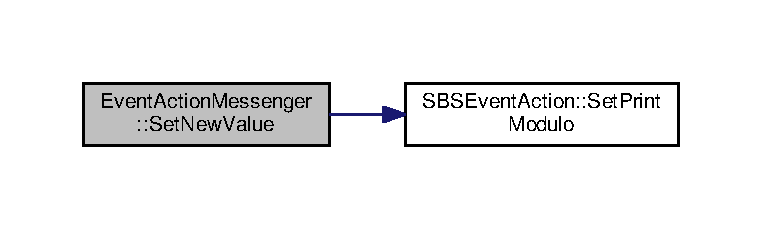
\includegraphics[width=350pt]{class_event_action_messenger_a5e0f6b3ab8d2b596b195b71f1111f934_cgraph}
\end{center}
\end{figure}




The documentation for this class was generated from the following files\-:\begin{DoxyCompactItemize}
\item 
g4work/\-Ecal/include/\hyperlink{_event_action_messenger_8hh}{Event\-Action\-Messenger.\-hh}\item 
g4work/\-Ecal/src/\hyperlink{_event_action_messenger_8cc}{Event\-Action\-Messenger.\-cc}\end{DoxyCompactItemize}

\hypertarget{class_physics_list}{\section{Physics\-List Class Reference}
\label{class_physics_list}\index{Physics\-List@{Physics\-List}}
}


{\ttfamily \#include $<$Physics\-List.\-hh$>$}

\subsection*{Public Member Functions}
\begin{DoxyCompactItemize}
\item 
\hyperlink{class_physics_list_aeecf835245a0b10c24e5e6c37cbb0dab}{Physics\-List} ()
\item 
virtual \hyperlink{class_physics_list_a6cff761e006f8d5c57f0beca0e7d61ae}{$\sim$\-Physics\-List} ()
\item 
void \hyperlink{class_physics_list_af7906507122c985d2da3e61c56efe60e}{Construct\-Particle} ()
\item 
void \hyperlink{class_physics_list_a9c08bc28eba2ae62104b967280901a3f}{Construct\-Process} ()
\item 
void \hyperlink{class_physics_list_a0ba901b82ae30657b109930645fe8017}{Set\-Cuts} ()
\end{DoxyCompactItemize}


\subsection{Detailed Description}


Definition at line 43 of file Physics\-List.\-hh.



\subsection{Constructor \& Destructor Documentation}
\hypertarget{class_physics_list_aeecf835245a0b10c24e5e6c37cbb0dab}{\index{Physics\-List@{Physics\-List}!Physics\-List@{Physics\-List}}
\index{Physics\-List@{Physics\-List}!PhysicsList@{Physics\-List}}
\subsubsection[{Physics\-List}]{\setlength{\rightskip}{0pt plus 5cm}Physics\-List\-::\-Physics\-List (
\begin{DoxyParamCaption}
{}
\end{DoxyParamCaption}
)}}\label{class_physics_list_aeecf835245a0b10c24e5e6c37cbb0dab}


Definition at line 48 of file Physics\-List.\-cc.

\hypertarget{class_physics_list_a6cff761e006f8d5c57f0beca0e7d61ae}{\index{Physics\-List@{Physics\-List}!$\sim$\-Physics\-List@{$\sim$\-Physics\-List}}
\index{$\sim$\-Physics\-List@{$\sim$\-Physics\-List}!PhysicsList@{Physics\-List}}
\subsubsection[{$\sim$\-Physics\-List}]{\setlength{\rightskip}{0pt plus 5cm}Physics\-List\-::$\sim$\-Physics\-List (
\begin{DoxyParamCaption}
{}
\end{DoxyParamCaption}
)\hspace{0.3cm}{\ttfamily [virtual]}}}\label{class_physics_list_a6cff761e006f8d5c57f0beca0e7d61ae}


Definition at line 57 of file Physics\-List.\-cc.



\subsection{Member Function Documentation}
\hypertarget{class_physics_list_af7906507122c985d2da3e61c56efe60e}{\index{Physics\-List@{Physics\-List}!Construct\-Particle@{Construct\-Particle}}
\index{Construct\-Particle@{Construct\-Particle}!PhysicsList@{Physics\-List}}
\subsubsection[{Construct\-Particle}]{\setlength{\rightskip}{0pt plus 5cm}void Physics\-List\-::\-Construct\-Particle (
\begin{DoxyParamCaption}
{}
\end{DoxyParamCaption}
)}}\label{class_physics_list_af7906507122c985d2da3e61c56efe60e}


Definition at line 62 of file Physics\-List.\-cc.

\hypertarget{class_physics_list_a9c08bc28eba2ae62104b967280901a3f}{\index{Physics\-List@{Physics\-List}!Construct\-Process@{Construct\-Process}}
\index{Construct\-Process@{Construct\-Process}!PhysicsList@{Physics\-List}}
\subsubsection[{Construct\-Process}]{\setlength{\rightskip}{0pt plus 5cm}void Physics\-List\-::\-Construct\-Process (
\begin{DoxyParamCaption}
{}
\end{DoxyParamCaption}
)}}\label{class_physics_list_a9c08bc28eba2ae62104b967280901a3f}


Definition at line 87 of file Physics\-List.\-cc.

\hypertarget{class_physics_list_a0ba901b82ae30657b109930645fe8017}{\index{Physics\-List@{Physics\-List}!Set\-Cuts@{Set\-Cuts}}
\index{Set\-Cuts@{Set\-Cuts}!PhysicsList@{Physics\-List}}
\subsubsection[{Set\-Cuts}]{\setlength{\rightskip}{0pt plus 5cm}void Physics\-List\-::\-Set\-Cuts (
\begin{DoxyParamCaption}
{}
\end{DoxyParamCaption}
)}}\label{class_physics_list_a0ba901b82ae30657b109930645fe8017}


Definition at line 208 of file Physics\-List.\-cc.



The documentation for this class was generated from the following files\-:\begin{DoxyCompactItemize}
\item 
g4work/\-Ecal/include/\hyperlink{_physics_list_8hh}{Physics\-List.\-hh}\item 
g4work/\-Ecal/src/\hyperlink{_physics_list_8cc}{Physics\-List.\-cc}\end{DoxyCompactItemize}

\hypertarget{class_primary_generator_messenger}{\section{Primary\-Generator\-Messenger Class Reference}
\label{class_primary_generator_messenger}\index{Primary\-Generator\-Messenger@{Primary\-Generator\-Messenger}}
}


{\ttfamily \#include $<$Primary\-Generator\-Messenger.\-hh$>$}

\subsection*{Public Member Functions}
\begin{DoxyCompactItemize}
\item 
\hyperlink{class_primary_generator_messenger_a89f388571f61f5cd51ca16e748061cd9}{Primary\-Generator\-Messenger} (\hyperlink{class_s_b_s_primary_generator_action}{S\-B\-S\-Primary\-Generator\-Action} $\ast$)
\item 
virtual \hyperlink{class_primary_generator_messenger_a5ae68a51211adc2b7dd1b29deb99124b}{$\sim$\-Primary\-Generator\-Messenger} ()
\item 
void \hyperlink{class_primary_generator_messenger_a0572868c7755cf589403cdad31af87c0}{Set\-New\-Value} (G4\-U\-Icommand $\ast$, G4\-String)
\end{DoxyCompactItemize}


\subsection{Detailed Description}


Definition at line 47 of file Primary\-Generator\-Messenger.\-hh.



\subsection{Constructor \& Destructor Documentation}
\hypertarget{class_primary_generator_messenger_a89f388571f61f5cd51ca16e748061cd9}{\index{Primary\-Generator\-Messenger@{Primary\-Generator\-Messenger}!Primary\-Generator\-Messenger@{Primary\-Generator\-Messenger}}
\index{Primary\-Generator\-Messenger@{Primary\-Generator\-Messenger}!PrimaryGeneratorMessenger@{Primary\-Generator\-Messenger}}
\subsubsection[{Primary\-Generator\-Messenger}]{\setlength{\rightskip}{0pt plus 5cm}Primary\-Generator\-Messenger\-::\-Primary\-Generator\-Messenger (
\begin{DoxyParamCaption}
\item[{{\bf S\-B\-S\-Primary\-Generator\-Action} $\ast$}]{Gun}
\end{DoxyParamCaption}
)}}\label{class_primary_generator_messenger_a89f388571f61f5cd51ca16e748061cd9}


Definition at line 43 of file Primary\-Generator\-Messenger.\-cc.

\hypertarget{class_primary_generator_messenger_a5ae68a51211adc2b7dd1b29deb99124b}{\index{Primary\-Generator\-Messenger@{Primary\-Generator\-Messenger}!$\sim$\-Primary\-Generator\-Messenger@{$\sim$\-Primary\-Generator\-Messenger}}
\index{$\sim$\-Primary\-Generator\-Messenger@{$\sim$\-Primary\-Generator\-Messenger}!PrimaryGeneratorMessenger@{Primary\-Generator\-Messenger}}
\subsubsection[{$\sim$\-Primary\-Generator\-Messenger}]{\setlength{\rightskip}{0pt plus 5cm}Primary\-Generator\-Messenger\-::$\sim$\-Primary\-Generator\-Messenger (
\begin{DoxyParamCaption}
{}
\end{DoxyParamCaption}
)\hspace{0.3cm}{\ttfamily [virtual]}}}\label{class_primary_generator_messenger_a5ae68a51211adc2b7dd1b29deb99124b}


Definition at line 61 of file Primary\-Generator\-Messenger.\-cc.



\subsection{Member Function Documentation}
\hypertarget{class_primary_generator_messenger_a0572868c7755cf589403cdad31af87c0}{\index{Primary\-Generator\-Messenger@{Primary\-Generator\-Messenger}!Set\-New\-Value@{Set\-New\-Value}}
\index{Set\-New\-Value@{Set\-New\-Value}!PrimaryGeneratorMessenger@{Primary\-Generator\-Messenger}}
\subsubsection[{Set\-New\-Value}]{\setlength{\rightskip}{0pt plus 5cm}void Primary\-Generator\-Messenger\-::\-Set\-New\-Value (
\begin{DoxyParamCaption}
\item[{G4\-U\-Icommand $\ast$}]{command, }
\item[{G4\-String}]{new\-Value}
\end{DoxyParamCaption}
)}}\label{class_primary_generator_messenger_a0572868c7755cf589403cdad31af87c0}


Definition at line 69 of file Primary\-Generator\-Messenger.\-cc.



Here is the call graph for this function\-:\nopagebreak
\begin{figure}[H]
\begin{center}
\leavevmode
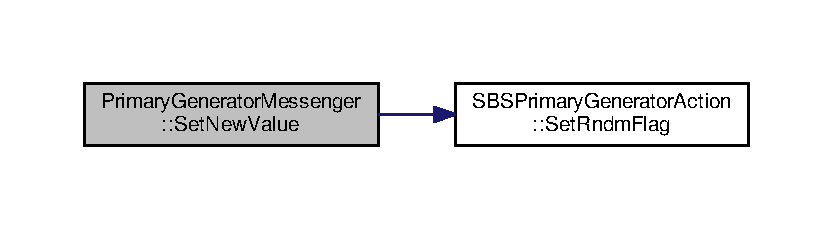
\includegraphics[width=350pt]{class_primary_generator_messenger_a0572868c7755cf589403cdad31af87c0_cgraph}
\end{center}
\end{figure}




The documentation for this class was generated from the following files\-:\begin{DoxyCompactItemize}
\item 
g4work/\-Ecal/include/\hyperlink{_primary_generator_messenger_8hh}{Primary\-Generator\-Messenger.\-hh}\item 
g4work/\-Ecal/src/\hyperlink{_primary_generator_messenger_8cc}{Primary\-Generator\-Messenger.\-cc}\end{DoxyCompactItemize}

\hypertarget{class_s_b_s_constants}{\section{S\-B\-S\-Constants Class Reference}
\label{class_s_b_s_constants}\index{S\-B\-S\-Constants@{S\-B\-S\-Constants}}
}


{\ttfamily \#include $<$S\-B\-S\-Constants.\-hh$>$}

\subsection*{Public Member Functions}
\begin{DoxyCompactItemize}
\item 
\hyperlink{class_s_b_s_constants_a049342309ed8be5bb9d9cbc761666e96}{S\-B\-S\-Constants} ()
\item 
\hyperlink{class_s_b_s_constants_ad4f98882743d06d212fccfc94a4626da}{$\sim$\-S\-B\-S\-Constants} ()
\end{DoxyCompactItemize}
\subsection*{Public Attributes}
\begin{DoxyCompactItemize}
\item 
G4double \hyperlink{class_s_b_s_constants_a29bf41467669a48826fb1bca3011820f}{Layer\-Thickness}
\item 
G4double \hyperlink{class_s_b_s_constants_a3cae081cf9c23144407404b801c21cf7}{Calor\-Thickness}
\item 
G4double \hyperlink{class_s_b_s_constants_a9b72c9889cfe808ce1d54dae2968f776}{World\-Size\-X}
\item 
G4double \hyperlink{class_s_b_s_constants_a8a08daf887918c2a3420c46b8adb17f0}{World\-Size\-Y\-Z}
\item 
G4double \hyperlink{class_s_b_s_constants_a88d873c312dc69a76d5e8b2c0f08ec25}{Proton\-Mass}
\end{DoxyCompactItemize}


\subsection{Detailed Description}


Definition at line 7 of file S\-B\-S\-Constants.\-hh.



\subsection{Constructor \& Destructor Documentation}
\hypertarget{class_s_b_s_constants_a049342309ed8be5bb9d9cbc761666e96}{\index{S\-B\-S\-Constants@{S\-B\-S\-Constants}!S\-B\-S\-Constants@{S\-B\-S\-Constants}}
\index{S\-B\-S\-Constants@{S\-B\-S\-Constants}!SBSConstants@{S\-B\-S\-Constants}}
\subsubsection[{S\-B\-S\-Constants}]{\setlength{\rightskip}{0pt plus 5cm}S\-B\-S\-Constants\-::\-S\-B\-S\-Constants (
\begin{DoxyParamCaption}
{}
\end{DoxyParamCaption}
)}}\label{class_s_b_s_constants_a049342309ed8be5bb9d9cbc761666e96}


Definition at line 4 of file S\-B\-S\-Constants.\-cc.

\hypertarget{class_s_b_s_constants_ad4f98882743d06d212fccfc94a4626da}{\index{S\-B\-S\-Constants@{S\-B\-S\-Constants}!$\sim$\-S\-B\-S\-Constants@{$\sim$\-S\-B\-S\-Constants}}
\index{$\sim$\-S\-B\-S\-Constants@{$\sim$\-S\-B\-S\-Constants}!SBSConstants@{S\-B\-S\-Constants}}
\subsubsection[{$\sim$\-S\-B\-S\-Constants}]{\setlength{\rightskip}{0pt plus 5cm}S\-B\-S\-Constants\-::$\sim$\-S\-B\-S\-Constants (
\begin{DoxyParamCaption}
{}
\end{DoxyParamCaption}
)}}\label{class_s_b_s_constants_ad4f98882743d06d212fccfc94a4626da}


Definition at line 43 of file S\-B\-S\-Constants.\-cc.



\subsection{Member Data Documentation}
\hypertarget{class_s_b_s_constants_a3cae081cf9c23144407404b801c21cf7}{\index{S\-B\-S\-Constants@{S\-B\-S\-Constants}!Calor\-Thickness@{Calor\-Thickness}}
\index{Calor\-Thickness@{Calor\-Thickness}!SBSConstants@{S\-B\-S\-Constants}}
\subsubsection[{Calor\-Thickness}]{\setlength{\rightskip}{0pt plus 5cm}G4double S\-B\-S\-Constants\-::\-Calor\-Thickness}}\label{class_s_b_s_constants_a3cae081cf9c23144407404b801c21cf7}


Definition at line 24 of file S\-B\-S\-Constants.\-hh.

\hypertarget{class_s_b_s_constants_a29bf41467669a48826fb1bca3011820f}{\index{S\-B\-S\-Constants@{S\-B\-S\-Constants}!Layer\-Thickness@{Layer\-Thickness}}
\index{Layer\-Thickness@{Layer\-Thickness}!SBSConstants@{S\-B\-S\-Constants}}
\subsubsection[{Layer\-Thickness}]{\setlength{\rightskip}{0pt plus 5cm}G4double S\-B\-S\-Constants\-::\-Layer\-Thickness}}\label{class_s_b_s_constants_a29bf41467669a48826fb1bca3011820f}


Definition at line 23 of file S\-B\-S\-Constants.\-hh.

\hypertarget{class_s_b_s_constants_a88d873c312dc69a76d5e8b2c0f08ec25}{\index{S\-B\-S\-Constants@{S\-B\-S\-Constants}!Proton\-Mass@{Proton\-Mass}}
\index{Proton\-Mass@{Proton\-Mass}!SBSConstants@{S\-B\-S\-Constants}}
\subsubsection[{Proton\-Mass}]{\setlength{\rightskip}{0pt plus 5cm}G4double S\-B\-S\-Constants\-::\-Proton\-Mass}}\label{class_s_b_s_constants_a88d873c312dc69a76d5e8b2c0f08ec25}


Definition at line 28 of file S\-B\-S\-Constants.\-hh.

\hypertarget{class_s_b_s_constants_a9b72c9889cfe808ce1d54dae2968f776}{\index{S\-B\-S\-Constants@{S\-B\-S\-Constants}!World\-Size\-X@{World\-Size\-X}}
\index{World\-Size\-X@{World\-Size\-X}!SBSConstants@{S\-B\-S\-Constants}}
\subsubsection[{World\-Size\-X}]{\setlength{\rightskip}{0pt plus 5cm}G4double S\-B\-S\-Constants\-::\-World\-Size\-X}}\label{class_s_b_s_constants_a9b72c9889cfe808ce1d54dae2968f776}


Definition at line 25 of file S\-B\-S\-Constants.\-hh.

\hypertarget{class_s_b_s_constants_a8a08daf887918c2a3420c46b8adb17f0}{\index{S\-B\-S\-Constants@{S\-B\-S\-Constants}!World\-Size\-Y\-Z@{World\-Size\-Y\-Z}}
\index{World\-Size\-Y\-Z@{World\-Size\-Y\-Z}!SBSConstants@{S\-B\-S\-Constants}}
\subsubsection[{World\-Size\-Y\-Z}]{\setlength{\rightskip}{0pt plus 5cm}G4double S\-B\-S\-Constants\-::\-World\-Size\-Y\-Z}}\label{class_s_b_s_constants_a8a08daf887918c2a3420c46b8adb17f0}


Definition at line 26 of file S\-B\-S\-Constants.\-hh.



The documentation for this class was generated from the following files\-:\begin{DoxyCompactItemize}
\item 
g4work/\-Ecal/include/\hyperlink{_s_b_s_constants_8hh}{S\-B\-S\-Constants.\-hh}\item 
g4work/\-Ecal/src/\hyperlink{_s_b_s_constants_8cc}{S\-B\-S\-Constants.\-cc}\end{DoxyCompactItemize}

\hypertarget{class_s_b_s_detector_construction}{\section{S\-B\-S\-Detector\-Construction Class Reference}
\label{class_s_b_s_detector_construction}\index{S\-B\-S\-Detector\-Construction@{S\-B\-S\-Detector\-Construction}}
}


{\ttfamily \#include $<$S\-B\-S\-Detector\-Construction.\-hh$>$}

\subsection*{Public Member Functions}
\begin{DoxyCompactItemize}
\item 
\hyperlink{class_s_b_s_detector_construction_ae6b5c301e30a26434ccc443ab944573a}{S\-B\-S\-Detector\-Construction} (G4\-Run\-Manager $\ast$)
\item 
\hyperlink{class_s_b_s_detector_construction_a5957da23069beacfdb6548da0fc2d559}{$\sim$\-S\-B\-S\-Detector\-Construction} ()
\item 
G4\-V\-Physical\-Volume $\ast$ \hyperlink{class_s_b_s_detector_construction_ac02815d916cb74b0095af5165d35fc46}{Construct} ()
\item 
void \hyperlink{class_s_b_s_detector_construction_ab3dded2f4f8043054fe56910a72fee77}{Set\-Mag\-Field} (G4double)
\item 
void \hyperlink{class_s_b_s_detector_construction_a9d797cd1388bbb03e46113bddd460e35}{Update\-Geometry} ()
\end{DoxyCompactItemize}


\subsection{Detailed Description}


Definition at line 59 of file S\-B\-S\-Detector\-Construction.\-hh.



\subsection{Constructor \& Destructor Documentation}
\hypertarget{class_s_b_s_detector_construction_ae6b5c301e30a26434ccc443ab944573a}{\index{S\-B\-S\-Detector\-Construction@{S\-B\-S\-Detector\-Construction}!S\-B\-S\-Detector\-Construction@{S\-B\-S\-Detector\-Construction}}
\index{S\-B\-S\-Detector\-Construction@{S\-B\-S\-Detector\-Construction}!SBSDetectorConstruction@{S\-B\-S\-Detector\-Construction}}
\subsubsection[{S\-B\-S\-Detector\-Construction}]{\setlength{\rightskip}{0pt plus 5cm}S\-B\-S\-Detector\-Construction\-::\-S\-B\-S\-Detector\-Construction (
\begin{DoxyParamCaption}
\item[{G4\-Run\-Manager $\ast$}]{run\-Manager}
\end{DoxyParamCaption}
)}}\label{class_s_b_s_detector_construction_ae6b5c301e30a26434ccc443ab944573a}


Definition at line 60 of file S\-B\-S\-Detector\-Construction.\-cc.

\hypertarget{class_s_b_s_detector_construction_a5957da23069beacfdb6548da0fc2d559}{\index{S\-B\-S\-Detector\-Construction@{S\-B\-S\-Detector\-Construction}!$\sim$\-S\-B\-S\-Detector\-Construction@{$\sim$\-S\-B\-S\-Detector\-Construction}}
\index{$\sim$\-S\-B\-S\-Detector\-Construction@{$\sim$\-S\-B\-S\-Detector\-Construction}!SBSDetectorConstruction@{S\-B\-S\-Detector\-Construction}}
\subsubsection[{$\sim$\-S\-B\-S\-Detector\-Construction}]{\setlength{\rightskip}{0pt plus 5cm}S\-B\-S\-Detector\-Construction\-::$\sim$\-S\-B\-S\-Detector\-Construction (
\begin{DoxyParamCaption}
{}
\end{DoxyParamCaption}
)}}\label{class_s_b_s_detector_construction_a5957da23069beacfdb6548da0fc2d559}


Definition at line 77 of file S\-B\-S\-Detector\-Construction.\-cc.



\subsection{Member Function Documentation}
\hypertarget{class_s_b_s_detector_construction_ac02815d916cb74b0095af5165d35fc46}{\index{S\-B\-S\-Detector\-Construction@{S\-B\-S\-Detector\-Construction}!Construct@{Construct}}
\index{Construct@{Construct}!SBSDetectorConstruction@{S\-B\-S\-Detector\-Construction}}
\subsubsection[{Construct}]{\setlength{\rightskip}{0pt plus 5cm}G4\-V\-Physical\-Volume $\ast$ S\-B\-S\-Detector\-Construction\-::\-Construct (
\begin{DoxyParamCaption}
{}
\end{DoxyParamCaption}
)}}\label{class_s_b_s_detector_construction_ac02815d916cb74b0095af5165d35fc46}


Definition at line 102 of file S\-B\-S\-Detector\-Construction.\-cc.



Here is the caller graph for this function\-:\nopagebreak
\begin{figure}[H]
\begin{center}
\leavevmode
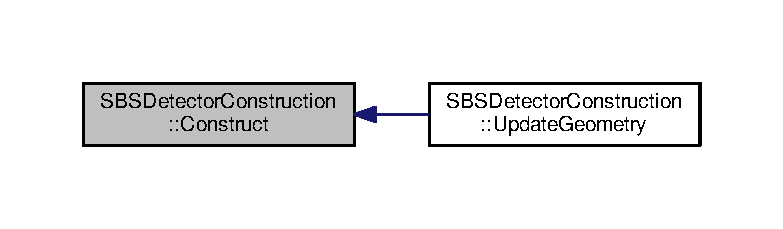
\includegraphics[width=350pt]{class_s_b_s_detector_construction_ac02815d916cb74b0095af5165d35fc46_icgraph}
\end{center}
\end{figure}


\hypertarget{class_s_b_s_detector_construction_ab3dded2f4f8043054fe56910a72fee77}{\index{S\-B\-S\-Detector\-Construction@{S\-B\-S\-Detector\-Construction}!Set\-Mag\-Field@{Set\-Mag\-Field}}
\index{Set\-Mag\-Field@{Set\-Mag\-Field}!SBSDetectorConstruction@{S\-B\-S\-Detector\-Construction}}
\subsubsection[{Set\-Mag\-Field}]{\setlength{\rightskip}{0pt plus 5cm}void S\-B\-S\-Detector\-Construction\-::\-Set\-Mag\-Field (
\begin{DoxyParamCaption}
\item[{G4double}]{field\-Value}
\end{DoxyParamCaption}
)}}\label{class_s_b_s_detector_construction_ab3dded2f4f8043054fe56910a72fee77}


Definition at line 174 of file S\-B\-S\-Detector\-Construction.\-cc.

\hypertarget{class_s_b_s_detector_construction_a9d797cd1388bbb03e46113bddd460e35}{\index{S\-B\-S\-Detector\-Construction@{S\-B\-S\-Detector\-Construction}!Update\-Geometry@{Update\-Geometry}}
\index{Update\-Geometry@{Update\-Geometry}!SBSDetectorConstruction@{S\-B\-S\-Detector\-Construction}}
\subsubsection[{Update\-Geometry}]{\setlength{\rightskip}{0pt plus 5cm}void S\-B\-S\-Detector\-Construction\-::\-Update\-Geometry (
\begin{DoxyParamCaption}
{}
\end{DoxyParamCaption}
)}}\label{class_s_b_s_detector_construction_a9d797cd1388bbb03e46113bddd460e35}


Definition at line 196 of file S\-B\-S\-Detector\-Construction.\-cc.



Here is the call graph for this function\-:\nopagebreak
\begin{figure}[H]
\begin{center}
\leavevmode
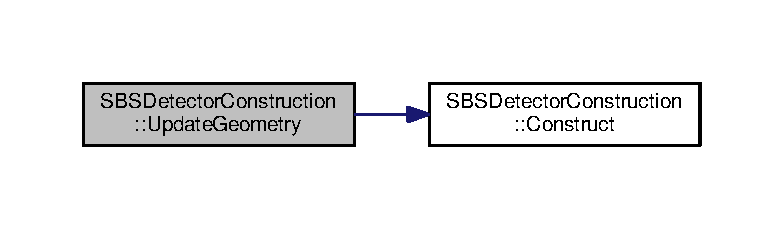
\includegraphics[width=350pt]{class_s_b_s_detector_construction_a9d797cd1388bbb03e46113bddd460e35_cgraph}
\end{center}
\end{figure}




The documentation for this class was generated from the following files\-:\begin{DoxyCompactItemize}
\item 
g4work/\-Ecal/include/\hyperlink{_s_b_s_detector_construction_8hh}{S\-B\-S\-Detector\-Construction.\-hh}\item 
g4work/\-Ecal/src/\hyperlink{_s_b_s_detector_construction_8cc}{S\-B\-S\-Detector\-Construction.\-cc}\end{DoxyCompactItemize}

\hypertarget{class_s_b_s_event_action}{\section{S\-B\-S\-Event\-Action Class Reference}
\label{class_s_b_s_event_action}\index{S\-B\-S\-Event\-Action@{S\-B\-S\-Event\-Action}}
}


{\ttfamily \#include $<$S\-B\-S\-Event\-Action.\-hh$>$}

\subsection*{Public Member Functions}
\begin{DoxyCompactItemize}
\item 
\hyperlink{class_s_b_s_event_action_a98038e4721f94fd604eb4ff6c95369be}{S\-B\-S\-Event\-Action} (\hyperlink{class_e_cal_analysis}{E\-Cal\-Analysis} $\ast$E\-Cal\-Handle)
\item 
virtual \hyperlink{class_s_b_s_event_action_a97eb694b4c25356ada559348fe45f8f4}{$\sim$\-S\-B\-S\-Event\-Action} ()
\item 
void \hyperlink{class_s_b_s_event_action_aaa6093b7ccf1bc47ab41832d91564266}{Begin\-Of\-Event\-Action} (const G4\-Event $\ast$)
\item 
void \hyperlink{class_s_b_s_event_action_aa77b8f0bcc8e7dd69fd0ab167d5dc20a}{End\-Of\-Event\-Action} (const G4\-Event $\ast$)
\item 
void \hyperlink{class_s_b_s_event_action_a34c1012298c01158013e5c63108e97d0}{Set\-Print\-Modulo} (G4int val)
\end{DoxyCompactItemize}


\subsection{Detailed Description}


Definition at line 48 of file S\-B\-S\-Event\-Action.\-hh.



\subsection{Constructor \& Destructor Documentation}
\hypertarget{class_s_b_s_event_action_a98038e4721f94fd604eb4ff6c95369be}{\index{S\-B\-S\-Event\-Action@{S\-B\-S\-Event\-Action}!S\-B\-S\-Event\-Action@{S\-B\-S\-Event\-Action}}
\index{S\-B\-S\-Event\-Action@{S\-B\-S\-Event\-Action}!SBSEventAction@{S\-B\-S\-Event\-Action}}
\subsubsection[{S\-B\-S\-Event\-Action}]{\setlength{\rightskip}{0pt plus 5cm}S\-B\-S\-Event\-Action\-::\-S\-B\-S\-Event\-Action (
\begin{DoxyParamCaption}
\item[{{\bf E\-Cal\-Analysis} $\ast$}]{E\-Cal\-Handle}
\end{DoxyParamCaption}
)}}\label{class_s_b_s_event_action_a98038e4721f94fd604eb4ff6c95369be}


Definition at line 52 of file S\-B\-S\-Event\-Action.\-cc.

\hypertarget{class_s_b_s_event_action_a97eb694b4c25356ada559348fe45f8f4}{\index{S\-B\-S\-Event\-Action@{S\-B\-S\-Event\-Action}!$\sim$\-S\-B\-S\-Event\-Action@{$\sim$\-S\-B\-S\-Event\-Action}}
\index{$\sim$\-S\-B\-S\-Event\-Action@{$\sim$\-S\-B\-S\-Event\-Action}!SBSEventAction@{S\-B\-S\-Event\-Action}}
\subsubsection[{$\sim$\-S\-B\-S\-Event\-Action}]{\setlength{\rightskip}{0pt plus 5cm}S\-B\-S\-Event\-Action\-::$\sim$\-S\-B\-S\-Event\-Action (
\begin{DoxyParamCaption}
{}
\end{DoxyParamCaption}
)\hspace{0.3cm}{\ttfamily [virtual]}}}\label{class_s_b_s_event_action_a97eb694b4c25356ada559348fe45f8f4}


Definition at line 70 of file S\-B\-S\-Event\-Action.\-cc.



\subsection{Member Function Documentation}
\hypertarget{class_s_b_s_event_action_aaa6093b7ccf1bc47ab41832d91564266}{\index{S\-B\-S\-Event\-Action@{S\-B\-S\-Event\-Action}!Begin\-Of\-Event\-Action@{Begin\-Of\-Event\-Action}}
\index{Begin\-Of\-Event\-Action@{Begin\-Of\-Event\-Action}!SBSEventAction@{S\-B\-S\-Event\-Action}}
\subsubsection[{Begin\-Of\-Event\-Action}]{\setlength{\rightskip}{0pt plus 5cm}void S\-B\-S\-Event\-Action\-::\-Begin\-Of\-Event\-Action (
\begin{DoxyParamCaption}
\item[{const G4\-Event $\ast$}]{evt}
\end{DoxyParamCaption}
)}}\label{class_s_b_s_event_action_aaa6093b7ccf1bc47ab41832d91564266}


Definition at line 77 of file S\-B\-S\-Event\-Action.\-cc.



Here is the call graph for this function\-:\nopagebreak
\begin{figure}[H]
\begin{center}
\leavevmode
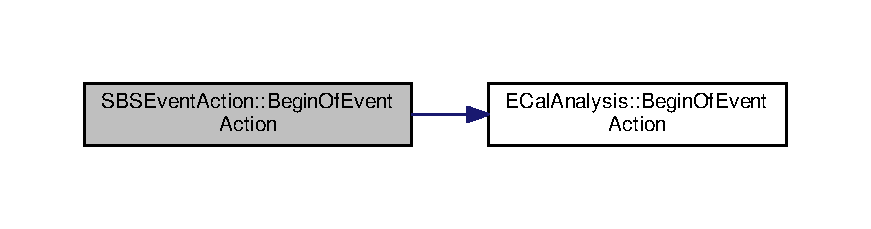
\includegraphics[width=350pt]{class_s_b_s_event_action_aaa6093b7ccf1bc47ab41832d91564266_cgraph}
\end{center}
\end{figure}


\hypertarget{class_s_b_s_event_action_aa77b8f0bcc8e7dd69fd0ab167d5dc20a}{\index{S\-B\-S\-Event\-Action@{S\-B\-S\-Event\-Action}!End\-Of\-Event\-Action@{End\-Of\-Event\-Action}}
\index{End\-Of\-Event\-Action@{End\-Of\-Event\-Action}!SBSEventAction@{S\-B\-S\-Event\-Action}}
\subsubsection[{End\-Of\-Event\-Action}]{\setlength{\rightskip}{0pt plus 5cm}void S\-B\-S\-Event\-Action\-::\-End\-Of\-Event\-Action (
\begin{DoxyParamCaption}
\item[{const G4\-Event $\ast$}]{an\-Event}
\end{DoxyParamCaption}
)}}\label{class_s_b_s_event_action_aa77b8f0bcc8e7dd69fd0ab167d5dc20a}


Definition at line 99 of file S\-B\-S\-Event\-Action.\-cc.



Here is the call graph for this function\-:\nopagebreak
\begin{figure}[H]
\begin{center}
\leavevmode
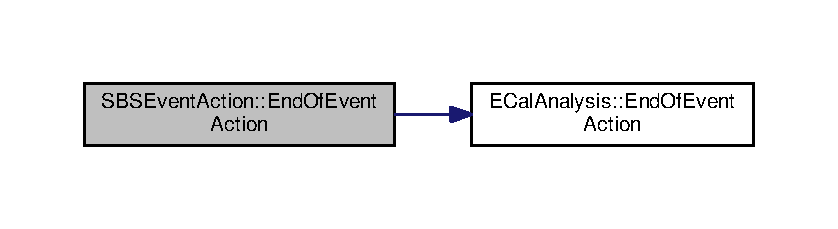
\includegraphics[width=350pt]{class_s_b_s_event_action_aa77b8f0bcc8e7dd69fd0ab167d5dc20a_cgraph}
\end{center}
\end{figure}


\hypertarget{class_s_b_s_event_action_a34c1012298c01158013e5c63108e97d0}{\index{S\-B\-S\-Event\-Action@{S\-B\-S\-Event\-Action}!Set\-Print\-Modulo@{Set\-Print\-Modulo}}
\index{Set\-Print\-Modulo@{Set\-Print\-Modulo}!SBSEventAction@{S\-B\-S\-Event\-Action}}
\subsubsection[{Set\-Print\-Modulo}]{\setlength{\rightskip}{0pt plus 5cm}void S\-B\-S\-Event\-Action\-::\-Set\-Print\-Modulo (
\begin{DoxyParamCaption}
\item[{G4int}]{val}
\end{DoxyParamCaption}
)\hspace{0.3cm}{\ttfamily [inline]}}}\label{class_s_b_s_event_action_a34c1012298c01158013e5c63108e97d0}


Definition at line 57 of file S\-B\-S\-Event\-Action.\-hh.



Here is the caller graph for this function\-:\nopagebreak
\begin{figure}[H]
\begin{center}
\leavevmode
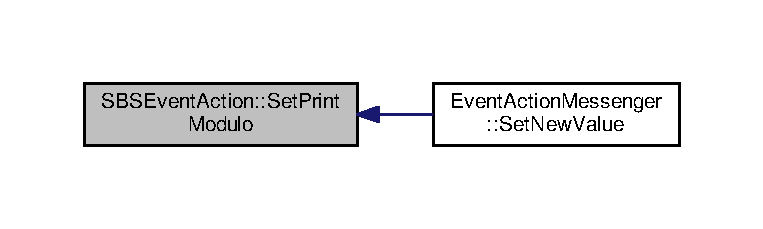
\includegraphics[width=350pt]{class_s_b_s_event_action_a34c1012298c01158013e5c63108e97d0_icgraph}
\end{center}
\end{figure}




The documentation for this class was generated from the following files\-:\begin{DoxyCompactItemize}
\item 
g4work/\-Ecal/include/\hyperlink{_s_b_s_event_action_8hh}{S\-B\-S\-Event\-Action.\-hh}\item 
g4work/\-Ecal/src/\hyperlink{_s_b_s_event_action_8cc}{S\-B\-S\-Event\-Action.\-cc}\end{DoxyCompactItemize}

\hypertarget{class_s_b_s_materials}{\section{S\-B\-S\-Materials Class Reference}
\label{class_s_b_s_materials}\index{S\-B\-S\-Materials@{S\-B\-S\-Materials}}
}


{\ttfamily \#include $<$S\-B\-S\-Materials.\-hh$>$}

\subsection*{Public Member Functions}
\begin{DoxyCompactItemize}
\item 
\hyperlink{class_s_b_s_materials_ade8845497bea2563e7210751fe65492d}{S\-B\-S\-Materials} ()
\item 
\hyperlink{class_s_b_s_materials_abe7bb67cc9753910b06c771201c6503b}{$\sim$\-S\-B\-S\-Materials} ()
\end{DoxyCompactItemize}
\subsection*{Public Attributes}
\begin{DoxyCompactItemize}
\item 
G4\-Material $\ast$ \hyperlink{class_s_b_s_materials_a9b29b0479ee57f534626d4b83aff7f78}{default\-Material}
\item 
G4\-Material $\ast$ \hyperlink{class_s_b_s_materials_ae273503caa4dd4f4d4cd8787d480faf4}{Vacuum}
\item 
G4\-Material $\ast$ \hyperlink{class_s_b_s_materials_aff3bcb06f66c199df9ef74ee7528d211}{Sci\-Material}
\item 
G4\-Material $\ast$ \hyperlink{class_s_b_s_materials_a3c95a0095e81186722814118b58aec0c}{Absorber\-Material}
\end{DoxyCompactItemize}


\subsection{Detailed Description}


Definition at line 7 of file S\-B\-S\-Materials.\-hh.



\subsection{Constructor \& Destructor Documentation}
\hypertarget{class_s_b_s_materials_ade8845497bea2563e7210751fe65492d}{\index{S\-B\-S\-Materials@{S\-B\-S\-Materials}!S\-B\-S\-Materials@{S\-B\-S\-Materials}}
\index{S\-B\-S\-Materials@{S\-B\-S\-Materials}!SBSMaterials@{S\-B\-S\-Materials}}
\subsubsection[{S\-B\-S\-Materials}]{\setlength{\rightskip}{0pt plus 5cm}S\-B\-S\-Materials\-::\-S\-B\-S\-Materials (
\begin{DoxyParamCaption}
{}
\end{DoxyParamCaption}
)}}\label{class_s_b_s_materials_ade8845497bea2563e7210751fe65492d}


Definition at line 9 of file S\-B\-S\-Materials.\-cc.

\hypertarget{class_s_b_s_materials_abe7bb67cc9753910b06c771201c6503b}{\index{S\-B\-S\-Materials@{S\-B\-S\-Materials}!$\sim$\-S\-B\-S\-Materials@{$\sim$\-S\-B\-S\-Materials}}
\index{$\sim$\-S\-B\-S\-Materials@{$\sim$\-S\-B\-S\-Materials}!SBSMaterials@{S\-B\-S\-Materials}}
\subsubsection[{$\sim$\-S\-B\-S\-Materials}]{\setlength{\rightskip}{0pt plus 5cm}S\-B\-S\-Materials\-::$\sim$\-S\-B\-S\-Materials (
\begin{DoxyParamCaption}
{}
\end{DoxyParamCaption}
)}}\label{class_s_b_s_materials_abe7bb67cc9753910b06c771201c6503b}


Definition at line 164 of file S\-B\-S\-Materials.\-cc.



\subsection{Member Data Documentation}
\hypertarget{class_s_b_s_materials_a3c95a0095e81186722814118b58aec0c}{\index{S\-B\-S\-Materials@{S\-B\-S\-Materials}!Absorber\-Material@{Absorber\-Material}}
\index{Absorber\-Material@{Absorber\-Material}!SBSMaterials@{S\-B\-S\-Materials}}
\subsubsection[{Absorber\-Material}]{\setlength{\rightskip}{0pt plus 5cm}G4\-Material$\ast$ S\-B\-S\-Materials\-::\-Absorber\-Material}}\label{class_s_b_s_materials_a3c95a0095e81186722814118b58aec0c}


Definition at line 17 of file S\-B\-S\-Materials.\-hh.

\hypertarget{class_s_b_s_materials_a9b29b0479ee57f534626d4b83aff7f78}{\index{S\-B\-S\-Materials@{S\-B\-S\-Materials}!default\-Material@{default\-Material}}
\index{default\-Material@{default\-Material}!SBSMaterials@{S\-B\-S\-Materials}}
\subsubsection[{default\-Material}]{\setlength{\rightskip}{0pt plus 5cm}G4\-Material$\ast$ S\-B\-S\-Materials\-::default\-Material}}\label{class_s_b_s_materials_a9b29b0479ee57f534626d4b83aff7f78}


Definition at line 14 of file S\-B\-S\-Materials.\-hh.

\hypertarget{class_s_b_s_materials_aff3bcb06f66c199df9ef74ee7528d211}{\index{S\-B\-S\-Materials@{S\-B\-S\-Materials}!Sci\-Material@{Sci\-Material}}
\index{Sci\-Material@{Sci\-Material}!SBSMaterials@{S\-B\-S\-Materials}}
\subsubsection[{Sci\-Material}]{\setlength{\rightskip}{0pt plus 5cm}G4\-Material$\ast$ S\-B\-S\-Materials\-::\-Sci\-Material}}\label{class_s_b_s_materials_aff3bcb06f66c199df9ef74ee7528d211}


Definition at line 16 of file S\-B\-S\-Materials.\-hh.

\hypertarget{class_s_b_s_materials_ae273503caa4dd4f4d4cd8787d480faf4}{\index{S\-B\-S\-Materials@{S\-B\-S\-Materials}!Vacuum@{Vacuum}}
\index{Vacuum@{Vacuum}!SBSMaterials@{S\-B\-S\-Materials}}
\subsubsection[{Vacuum}]{\setlength{\rightskip}{0pt plus 5cm}G4\-Material$\ast$ S\-B\-S\-Materials\-::\-Vacuum}}\label{class_s_b_s_materials_ae273503caa4dd4f4d4cd8787d480faf4}


Definition at line 15 of file S\-B\-S\-Materials.\-hh.



The documentation for this class was generated from the following files\-:\begin{DoxyCompactItemize}
\item 
g4work/\-Ecal/include/\hyperlink{_s_b_s_materials_8hh}{S\-B\-S\-Materials.\-hh}\item 
g4work/\-Ecal/src/\hyperlink{_s_b_s_materials_8cc}{S\-B\-S\-Materials.\-cc}\end{DoxyCompactItemize}

\hypertarget{class_s_b_s_primary_generator_action}{\section{S\-B\-S\-Primary\-Generator\-Action Class Reference}
\label{class_s_b_s_primary_generator_action}\index{S\-B\-S\-Primary\-Generator\-Action@{S\-B\-S\-Primary\-Generator\-Action}}
}


{\ttfamily \#include $<$S\-B\-S\-Primary\-Generator\-Action.\-hh$>$}

\subsection*{Public Member Functions}
\begin{DoxyCompactItemize}
\item 
\hyperlink{class_s_b_s_primary_generator_action_a16d7adf8604fb255bc103c3e9235a43e}{S\-B\-S\-Primary\-Generator\-Action} ()
\item 
virtual \hyperlink{class_s_b_s_primary_generator_action_a88223d1c7c2b102878d929e8a48b4c1a}{$\sim$\-S\-B\-S\-Primary\-Generator\-Action} ()
\item 
void \hyperlink{class_s_b_s_primary_generator_action_ab2c619962b7b1ac4fcf1814be43f444c}{Generate\-Primaries} (G4\-Event $\ast$)
\item 
void \hyperlink{class_s_b_s_primary_generator_action_acdd868b7328f35d17676997c458977e3}{Set\-Rndm\-Flag} (G4\-String val)
\end{DoxyCompactItemize}


\subsection{Detailed Description}


Definition at line 48 of file S\-B\-S\-Primary\-Generator\-Action.\-hh.



\subsection{Constructor \& Destructor Documentation}
\hypertarget{class_s_b_s_primary_generator_action_a16d7adf8604fb255bc103c3e9235a43e}{\index{S\-B\-S\-Primary\-Generator\-Action@{S\-B\-S\-Primary\-Generator\-Action}!S\-B\-S\-Primary\-Generator\-Action@{S\-B\-S\-Primary\-Generator\-Action}}
\index{S\-B\-S\-Primary\-Generator\-Action@{S\-B\-S\-Primary\-Generator\-Action}!SBSPrimaryGeneratorAction@{S\-B\-S\-Primary\-Generator\-Action}}
\subsubsection[{S\-B\-S\-Primary\-Generator\-Action}]{\setlength{\rightskip}{0pt plus 5cm}S\-B\-S\-Primary\-Generator\-Action\-::\-S\-B\-S\-Primary\-Generator\-Action (
\begin{DoxyParamCaption}
{}
\end{DoxyParamCaption}
)}}\label{class_s_b_s_primary_generator_action_a16d7adf8604fb255bc103c3e9235a43e}


Definition at line 52 of file S\-B\-S\-Primary\-Generator\-Action.\-cc.

\hypertarget{class_s_b_s_primary_generator_action_a88223d1c7c2b102878d929e8a48b4c1a}{\index{S\-B\-S\-Primary\-Generator\-Action@{S\-B\-S\-Primary\-Generator\-Action}!$\sim$\-S\-B\-S\-Primary\-Generator\-Action@{$\sim$\-S\-B\-S\-Primary\-Generator\-Action}}
\index{$\sim$\-S\-B\-S\-Primary\-Generator\-Action@{$\sim$\-S\-B\-S\-Primary\-Generator\-Action}!SBSPrimaryGeneratorAction@{S\-B\-S\-Primary\-Generator\-Action}}
\subsubsection[{$\sim$\-S\-B\-S\-Primary\-Generator\-Action}]{\setlength{\rightskip}{0pt plus 5cm}S\-B\-S\-Primary\-Generator\-Action\-::$\sim$\-S\-B\-S\-Primary\-Generator\-Action (
\begin{DoxyParamCaption}
{}
\end{DoxyParamCaption}
)\hspace{0.3cm}{\ttfamily [virtual]}}}\label{class_s_b_s_primary_generator_action_a88223d1c7c2b102878d929e8a48b4c1a}


Definition at line 85 of file S\-B\-S\-Primary\-Generator\-Action.\-cc.



\subsection{Member Function Documentation}
\hypertarget{class_s_b_s_primary_generator_action_ab2c619962b7b1ac4fcf1814be43f444c}{\index{S\-B\-S\-Primary\-Generator\-Action@{S\-B\-S\-Primary\-Generator\-Action}!Generate\-Primaries@{Generate\-Primaries}}
\index{Generate\-Primaries@{Generate\-Primaries}!SBSPrimaryGeneratorAction@{S\-B\-S\-Primary\-Generator\-Action}}
\subsubsection[{Generate\-Primaries}]{\setlength{\rightskip}{0pt plus 5cm}void S\-B\-S\-Primary\-Generator\-Action\-::\-Generate\-Primaries (
\begin{DoxyParamCaption}
\item[{G4\-Event $\ast$}]{an\-Event}
\end{DoxyParamCaption}
)}}\label{class_s_b_s_primary_generator_action_ab2c619962b7b1ac4fcf1814be43f444c}


Definition at line 94 of file S\-B\-S\-Primary\-Generator\-Action.\-cc.

\hypertarget{class_s_b_s_primary_generator_action_acdd868b7328f35d17676997c458977e3}{\index{S\-B\-S\-Primary\-Generator\-Action@{S\-B\-S\-Primary\-Generator\-Action}!Set\-Rndm\-Flag@{Set\-Rndm\-Flag}}
\index{Set\-Rndm\-Flag@{Set\-Rndm\-Flag}!SBSPrimaryGeneratorAction@{S\-B\-S\-Primary\-Generator\-Action}}
\subsubsection[{Set\-Rndm\-Flag}]{\setlength{\rightskip}{0pt plus 5cm}void S\-B\-S\-Primary\-Generator\-Action\-::\-Set\-Rndm\-Flag (
\begin{DoxyParamCaption}
\item[{G4\-String}]{val}
\end{DoxyParamCaption}
)\hspace{0.3cm}{\ttfamily [inline]}}}\label{class_s_b_s_primary_generator_action_acdd868b7328f35d17676997c458977e3}


Definition at line 55 of file S\-B\-S\-Primary\-Generator\-Action.\-hh.



Here is the caller graph for this function\-:\nopagebreak
\begin{figure}[H]
\begin{center}
\leavevmode
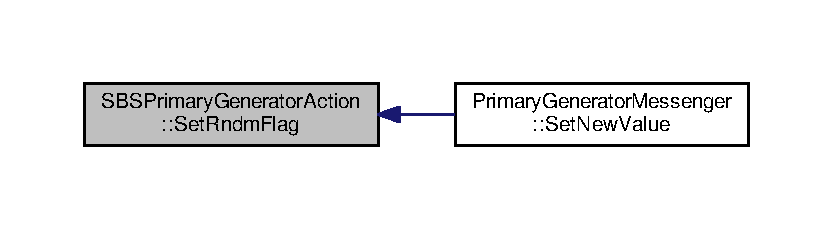
\includegraphics[width=350pt]{class_s_b_s_primary_generator_action_acdd868b7328f35d17676997c458977e3_icgraph}
\end{center}
\end{figure}




The documentation for this class was generated from the following files\-:\begin{DoxyCompactItemize}
\item 
g4work/\-Ecal/include/\hyperlink{_s_b_s_primary_generator_action_8hh}{S\-B\-S\-Primary\-Generator\-Action.\-hh}\item 
g4work/\-Ecal/src/\hyperlink{_s_b_s_primary_generator_action_8cc}{S\-B\-S\-Primary\-Generator\-Action.\-cc}\end{DoxyCompactItemize}

\hypertarget{class_s_b_s_run_action}{\section{S\-B\-S\-Run\-Action Class Reference}
\label{class_s_b_s_run_action}\index{S\-B\-S\-Run\-Action@{S\-B\-S\-Run\-Action}}
}


{\ttfamily \#include $<$S\-B\-S\-Run\-Action.\-hh$>$}

\subsection*{Public Member Functions}
\begin{DoxyCompactItemize}
\item 
\hyperlink{class_s_b_s_run_action_aceed8fd88c981dc05b8481409f4810a2}{S\-B\-S\-Run\-Action} (\hyperlink{class_e_cal_analysis}{E\-Cal\-Analysis} $\ast$E\-Cal\-Handle)
\item 
virtual \hyperlink{class_s_b_s_run_action_a1df41f7f362965676ff2bc079ced824e}{$\sim$\-S\-B\-S\-Run\-Action} ()
\item 
void \hyperlink{class_s_b_s_run_action_a4a08c62f1efc58c1b8f5cc1e92227e59}{Begin\-Of\-Run\-Action} (const G4\-Run $\ast$)
\item 
void \hyperlink{class_s_b_s_run_action_a8be9aad9176d85ab222c69f875ec2f8b}{End\-Of\-Run\-Action} (const G4\-Run $\ast$)
\end{DoxyCompactItemize}


\subsection{Detailed Description}


Definition at line 51 of file S\-B\-S\-Run\-Action.\-hh.



\subsection{Constructor \& Destructor Documentation}
\hypertarget{class_s_b_s_run_action_aceed8fd88c981dc05b8481409f4810a2}{\index{S\-B\-S\-Run\-Action@{S\-B\-S\-Run\-Action}!S\-B\-S\-Run\-Action@{S\-B\-S\-Run\-Action}}
\index{S\-B\-S\-Run\-Action@{S\-B\-S\-Run\-Action}!SBSRunAction@{S\-B\-S\-Run\-Action}}
\subsubsection[{S\-B\-S\-Run\-Action}]{\setlength{\rightskip}{0pt plus 5cm}S\-B\-S\-Run\-Action\-::\-S\-B\-S\-Run\-Action (
\begin{DoxyParamCaption}
\item[{{\bf E\-Cal\-Analysis} $\ast$}]{E\-Cal\-Handle}
\end{DoxyParamCaption}
)}}\label{class_s_b_s_run_action_aceed8fd88c981dc05b8481409f4810a2}


Definition at line 43 of file S\-B\-S\-Run\-Action.\-cc.

\hypertarget{class_s_b_s_run_action_a1df41f7f362965676ff2bc079ced824e}{\index{S\-B\-S\-Run\-Action@{S\-B\-S\-Run\-Action}!$\sim$\-S\-B\-S\-Run\-Action@{$\sim$\-S\-B\-S\-Run\-Action}}
\index{$\sim$\-S\-B\-S\-Run\-Action@{$\sim$\-S\-B\-S\-Run\-Action}!SBSRunAction@{S\-B\-S\-Run\-Action}}
\subsubsection[{$\sim$\-S\-B\-S\-Run\-Action}]{\setlength{\rightskip}{0pt plus 5cm}S\-B\-S\-Run\-Action\-::$\sim$\-S\-B\-S\-Run\-Action (
\begin{DoxyParamCaption}
{}
\end{DoxyParamCaption}
)\hspace{0.3cm}{\ttfamily [virtual]}}}\label{class_s_b_s_run_action_a1df41f7f362965676ff2bc079ced824e}


Definition at line 53 of file S\-B\-S\-Run\-Action.\-cc.



\subsection{Member Function Documentation}
\hypertarget{class_s_b_s_run_action_a4a08c62f1efc58c1b8f5cc1e92227e59}{\index{S\-B\-S\-Run\-Action@{S\-B\-S\-Run\-Action}!Begin\-Of\-Run\-Action@{Begin\-Of\-Run\-Action}}
\index{Begin\-Of\-Run\-Action@{Begin\-Of\-Run\-Action}!SBSRunAction@{S\-B\-S\-Run\-Action}}
\subsubsection[{Begin\-Of\-Run\-Action}]{\setlength{\rightskip}{0pt plus 5cm}void S\-B\-S\-Run\-Action\-::\-Begin\-Of\-Run\-Action (
\begin{DoxyParamCaption}
\item[{const G4\-Run $\ast$}]{a\-Run}
\end{DoxyParamCaption}
)}}\label{class_s_b_s_run_action_a4a08c62f1efc58c1b8f5cc1e92227e59}


Definition at line 61 of file S\-B\-S\-Run\-Action.\-cc.



Here is the call graph for this function\-:\nopagebreak
\begin{figure}[H]
\begin{center}
\leavevmode
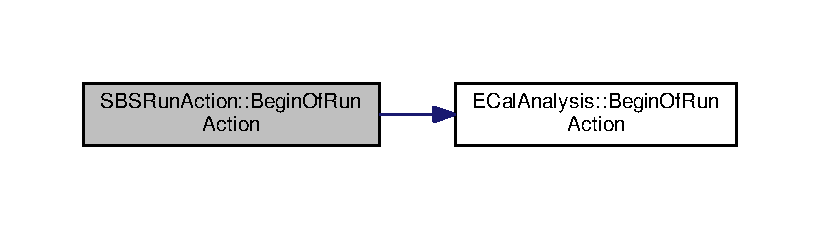
\includegraphics[width=350pt]{class_s_b_s_run_action_a4a08c62f1efc58c1b8f5cc1e92227e59_cgraph}
\end{center}
\end{figure}


\hypertarget{class_s_b_s_run_action_a8be9aad9176d85ab222c69f875ec2f8b}{\index{S\-B\-S\-Run\-Action@{S\-B\-S\-Run\-Action}!End\-Of\-Run\-Action@{End\-Of\-Run\-Action}}
\index{End\-Of\-Run\-Action@{End\-Of\-Run\-Action}!SBSRunAction@{S\-B\-S\-Run\-Action}}
\subsubsection[{End\-Of\-Run\-Action}]{\setlength{\rightskip}{0pt plus 5cm}void S\-B\-S\-Run\-Action\-::\-End\-Of\-Run\-Action (
\begin{DoxyParamCaption}
\item[{const G4\-Run $\ast$}]{a\-Run}
\end{DoxyParamCaption}
)}}\label{class_s_b_s_run_action_a8be9aad9176d85ab222c69f875ec2f8b}


Definition at line 96 of file S\-B\-S\-Run\-Action.\-cc.



Here is the call graph for this function\-:\nopagebreak
\begin{figure}[H]
\begin{center}
\leavevmode
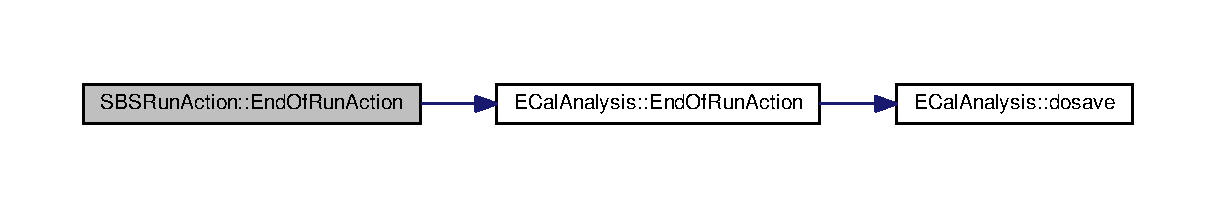
\includegraphics[width=350pt]{class_s_b_s_run_action_a8be9aad9176d85ab222c69f875ec2f8b_cgraph}
\end{center}
\end{figure}




The documentation for this class was generated from the following files\-:\begin{DoxyCompactItemize}
\item 
g4work/\-Ecal/include/\hyperlink{_s_b_s_run_action_8hh}{S\-B\-S\-Run\-Action.\-hh}\item 
g4work/\-Ecal/src/\hyperlink{_s_b_s_run_action_8cc}{S\-B\-S\-Run\-Action.\-cc}\end{DoxyCompactItemize}

\hypertarget{class_s_b_s_stepping_action}{\section{S\-B\-S\-Stepping\-Action Class Reference}
\label{class_s_b_s_stepping_action}\index{S\-B\-S\-Stepping\-Action@{S\-B\-S\-Stepping\-Action}}
}


{\ttfamily \#include $<$S\-B\-S\-Stepping\-Action.\-hh$>$}

\subsection*{Public Member Functions}
\begin{DoxyCompactItemize}
\item 
\hyperlink{class_s_b_s_stepping_action_a5eb7feae52b6a44fadfb27613657dbf1}{S\-B\-S\-Stepping\-Action} (\hyperlink{class_e_cal_analysis}{E\-Cal\-Analysis} $\ast$E\-Cal\-Handle)
\item 
\hyperlink{class_s_b_s_stepping_action_aa6adaccc5142568d7d0a9c219a2740e9}{$\sim$\-S\-B\-S\-Stepping\-Action} ()
\item 
void \hyperlink{class_s_b_s_stepping_action_af06b2717d7c732ce43560b4f4b4091e2}{User\-Stepping\-Action} (const G4\-Step $\ast$)
\end{DoxyCompactItemize}


\subsection{Detailed Description}


Definition at line 53 of file S\-B\-S\-Stepping\-Action.\-hh.



\subsection{Constructor \& Destructor Documentation}
\hypertarget{class_s_b_s_stepping_action_a5eb7feae52b6a44fadfb27613657dbf1}{\index{S\-B\-S\-Stepping\-Action@{S\-B\-S\-Stepping\-Action}!S\-B\-S\-Stepping\-Action@{S\-B\-S\-Stepping\-Action}}
\index{S\-B\-S\-Stepping\-Action@{S\-B\-S\-Stepping\-Action}!SBSSteppingAction@{S\-B\-S\-Stepping\-Action}}
\subsubsection[{S\-B\-S\-Stepping\-Action}]{\setlength{\rightskip}{0pt plus 5cm}S\-B\-S\-Stepping\-Action\-::\-S\-B\-S\-Stepping\-Action (
\begin{DoxyParamCaption}
\item[{{\bf E\-Cal\-Analysis} $\ast$}]{E\-Cal\-Handle}
\end{DoxyParamCaption}
)}}\label{class_s_b_s_stepping_action_a5eb7feae52b6a44fadfb27613657dbf1}


Definition at line 51 of file S\-B\-S\-Stepping\-Action.\-cc.

\hypertarget{class_s_b_s_stepping_action_aa6adaccc5142568d7d0a9c219a2740e9}{\index{S\-B\-S\-Stepping\-Action@{S\-B\-S\-Stepping\-Action}!$\sim$\-S\-B\-S\-Stepping\-Action@{$\sim$\-S\-B\-S\-Stepping\-Action}}
\index{$\sim$\-S\-B\-S\-Stepping\-Action@{$\sim$\-S\-B\-S\-Stepping\-Action}!SBSSteppingAction@{S\-B\-S\-Stepping\-Action}}
\subsubsection[{$\sim$\-S\-B\-S\-Stepping\-Action}]{\setlength{\rightskip}{0pt plus 5cm}S\-B\-S\-Stepping\-Action\-::$\sim$\-S\-B\-S\-Stepping\-Action (
\begin{DoxyParamCaption}
{}
\end{DoxyParamCaption}
)}}\label{class_s_b_s_stepping_action_aa6adaccc5142568d7d0a9c219a2740e9}


Definition at line 77 of file S\-B\-S\-Stepping\-Action.\-cc.



\subsection{Member Function Documentation}
\hypertarget{class_s_b_s_stepping_action_af06b2717d7c732ce43560b4f4b4091e2}{\index{S\-B\-S\-Stepping\-Action@{S\-B\-S\-Stepping\-Action}!User\-Stepping\-Action@{User\-Stepping\-Action}}
\index{User\-Stepping\-Action@{User\-Stepping\-Action}!SBSSteppingAction@{S\-B\-S\-Stepping\-Action}}
\subsubsection[{User\-Stepping\-Action}]{\setlength{\rightskip}{0pt plus 5cm}void S\-B\-S\-Stepping\-Action\-::\-User\-Stepping\-Action (
\begin{DoxyParamCaption}
\item[{const G4\-Step $\ast$}]{a\-Step}
\end{DoxyParamCaption}
)}}\label{class_s_b_s_stepping_action_af06b2717d7c732ce43560b4f4b4091e2}


Definition at line 86 of file S\-B\-S\-Stepping\-Action.\-cc.



Here is the call graph for this function\-:\nopagebreak
\begin{figure}[H]
\begin{center}
\leavevmode
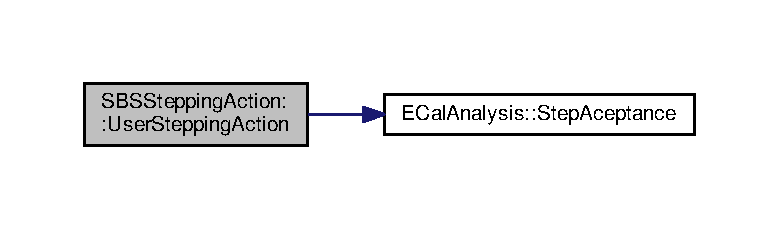
\includegraphics[width=350pt]{class_s_b_s_stepping_action_af06b2717d7c732ce43560b4f4b4091e2_cgraph}
\end{center}
\end{figure}




The documentation for this class was generated from the following files\-:\begin{DoxyCompactItemize}
\item 
g4work/\-Ecal/include/\hyperlink{_s_b_s_stepping_action_8hh}{S\-B\-S\-Stepping\-Action.\-hh}\item 
g4work/\-Ecal/src/\hyperlink{_s_b_s_stepping_action_8cc}{S\-B\-S\-Stepping\-Action.\-cc}\end{DoxyCompactItemize}

\hypertarget{class_s_b_s_variables}{\section{S\-B\-S\-Variables Class Reference}
\label{class_s_b_s_variables}\index{S\-B\-S\-Variables@{S\-B\-S\-Variables}}
}


{\ttfamily \#include $<$S\-B\-S\-Variables.\-hh$>$}

\subsection*{Public Member Functions}
\begin{DoxyCompactItemize}
\item 
\hyperlink{class_s_b_s_variables_afd6b16b0acdea92ad9cc5b311c57ba87}{S\-B\-S\-Variables} ()
\item 
\hyperlink{class_s_b_s_variables_af4fc969fc880e0a390b3eaafae0678a2}{$\sim$\-S\-B\-S\-Variables} ()
\item 
G4int \hyperlink{class_s_b_s_variables_a2d26940b705eab7e5a0eb11d4ff28dd5}{Load\-From\-File} (G4\-String File\-Name)
\end{DoxyCompactItemize}
\subsection*{Public Attributes}
\begin{DoxyCompactItemize}
\item 
G4double \hyperlink{class_s_b_s_variables_ac18998a9e16bed4d4737bd3fdbe3032e}{Lead\-Thickness}
\item 
G4double \hyperlink{class_s_b_s_variables_abb259dd81111497ec4db2fe9199f2d01}{Scint\-Thickness}
\item 
G4int \hyperlink{class_s_b_s_variables_adec94678029bfd057c6ba3daabe6f5a3}{Nb\-Of\-Layers}
\item 
G4double \hyperlink{class_s_b_s_variables_a92e4bb3f201e0cff282ca71215348156}{Cal\-Mod\-Size\-X\-Y}
\item 
G4int \hyperlink{class_s_b_s_variables_adc90201ebd65e3b3366b1b6f4dff5ebf}{Nb\-Of\-Calo\-Columns}
\item 
G4int \hyperlink{class_s_b_s_variables_acf7deca6d17faac95752ce05c0c49d55}{Nb\-Of\-Calo\-Rows}
\item 
G4bool \hyperlink{class_s_b_s_variables_a370739e528c9193ac1da6d4fed91c882}{E\-Cal\-Detail}
\item 
G4double \hyperlink{class_s_b_s_variables_a3286bfb8c9f691a7315a5c97c7ea1adc}{Ele\-Ang}
\item 
G4double \hyperlink{class_s_b_s_variables_ad7c0c85364e09e7dc5f7d687bf7fbbf4}{E\-Cal\-Dis}
\item 
G4\-String \hyperlink{class_s_b_s_variables_a47b76d8c38f66e49d9b321ef066b28e9}{File\-Name\-Suffix}
\item 
G4\-Three\-Vector \hyperlink{class_s_b_s_variables_a3c76a8b893d04a78ff94f46cc80a7932}{Target}
\item 
G4int \hyperlink{class_s_b_s_variables_ab416f097e1de50c1bbc462d5908f6b5d}{Reaction\-Case}
\item 
G4double \hyperlink{class_s_b_s_variables_a690e4d01c59328ad6ac6f53a9b6cc3e7}{Energy\-Beam}
\item 
G4int \hyperlink{class_s_b_s_variables_af10311ab957c982d3916c1d838162786}{n\-K}
\item 
G4\-String \hyperlink{class_s_b_s_variables_a0920a3979aa1c25c139d6a0f13669b00}{Reaction\-Particle} \mbox{[}4\mbox{]}
\end{DoxyCompactItemize}


\subsection{Detailed Description}


Definition at line 15 of file S\-B\-S\-Variables.\-hh.



\subsection{Constructor \& Destructor Documentation}
\hypertarget{class_s_b_s_variables_afd6b16b0acdea92ad9cc5b311c57ba87}{\index{S\-B\-S\-Variables@{S\-B\-S\-Variables}!S\-B\-S\-Variables@{S\-B\-S\-Variables}}
\index{S\-B\-S\-Variables@{S\-B\-S\-Variables}!SBSVariables@{S\-B\-S\-Variables}}
\subsubsection[{S\-B\-S\-Variables}]{\setlength{\rightskip}{0pt plus 5cm}S\-B\-S\-Variables\-::\-S\-B\-S\-Variables (
\begin{DoxyParamCaption}
{}
\end{DoxyParamCaption}
)}}\label{class_s_b_s_variables_afd6b16b0acdea92ad9cc5b311c57ba87}


Definition at line 45 of file S\-B\-S\-Variables.\-cc.

\hypertarget{class_s_b_s_variables_af4fc969fc880e0a390b3eaafae0678a2}{\index{S\-B\-S\-Variables@{S\-B\-S\-Variables}!$\sim$\-S\-B\-S\-Variables@{$\sim$\-S\-B\-S\-Variables}}
\index{$\sim$\-S\-B\-S\-Variables@{$\sim$\-S\-B\-S\-Variables}!SBSVariables@{S\-B\-S\-Variables}}
\subsubsection[{$\sim$\-S\-B\-S\-Variables}]{\setlength{\rightskip}{0pt plus 5cm}S\-B\-S\-Variables\-::$\sim$\-S\-B\-S\-Variables (
\begin{DoxyParamCaption}
{}
\end{DoxyParamCaption}
)}}\label{class_s_b_s_variables_af4fc969fc880e0a390b3eaafae0678a2}


Definition at line 120 of file S\-B\-S\-Variables.\-cc.



\subsection{Member Function Documentation}
\hypertarget{class_s_b_s_variables_a2d26940b705eab7e5a0eb11d4ff28dd5}{\index{S\-B\-S\-Variables@{S\-B\-S\-Variables}!Load\-From\-File@{Load\-From\-File}}
\index{Load\-From\-File@{Load\-From\-File}!SBSVariables@{S\-B\-S\-Variables}}
\subsubsection[{Load\-From\-File}]{\setlength{\rightskip}{0pt plus 5cm}G4int S\-B\-S\-Variables\-::\-Load\-From\-File (
\begin{DoxyParamCaption}
\item[{G4\-String}]{File\-Name}
\end{DoxyParamCaption}
)}}\label{class_s_b_s_variables_a2d26940b705eab7e5a0eb11d4ff28dd5}


Definition at line 126 of file S\-B\-S\-Variables.\-cc.



Here is the caller graph for this function\-:\nopagebreak
\begin{figure}[H]
\begin{center}
\leavevmode
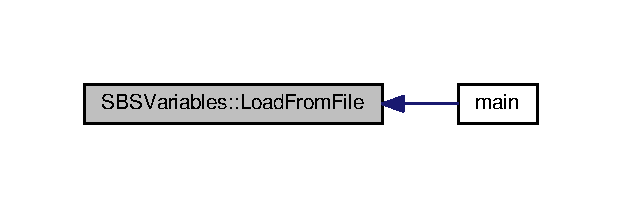
\includegraphics[width=298pt]{class_s_b_s_variables_a2d26940b705eab7e5a0eb11d4ff28dd5_icgraph}
\end{center}
\end{figure}




\subsection{Member Data Documentation}
\hypertarget{class_s_b_s_variables_a92e4bb3f201e0cff282ca71215348156}{\index{S\-B\-S\-Variables@{S\-B\-S\-Variables}!Cal\-Mod\-Size\-X\-Y@{Cal\-Mod\-Size\-X\-Y}}
\index{Cal\-Mod\-Size\-X\-Y@{Cal\-Mod\-Size\-X\-Y}!SBSVariables@{S\-B\-S\-Variables}}
\subsubsection[{Cal\-Mod\-Size\-X\-Y}]{\setlength{\rightskip}{0pt plus 5cm}G4double S\-B\-S\-Variables\-::\-Cal\-Mod\-Size\-X\-Y}}\label{class_s_b_s_variables_a92e4bb3f201e0cff282ca71215348156}


Definition at line 29 of file S\-B\-S\-Variables.\-hh.

\hypertarget{class_s_b_s_variables_a370739e528c9193ac1da6d4fed91c882}{\index{S\-B\-S\-Variables@{S\-B\-S\-Variables}!E\-Cal\-Detail@{E\-Cal\-Detail}}
\index{E\-Cal\-Detail@{E\-Cal\-Detail}!SBSVariables@{S\-B\-S\-Variables}}
\subsubsection[{E\-Cal\-Detail}]{\setlength{\rightskip}{0pt plus 5cm}G4bool S\-B\-S\-Variables\-::\-E\-Cal\-Detail}}\label{class_s_b_s_variables_a370739e528c9193ac1da6d4fed91c882}


Definition at line 33 of file S\-B\-S\-Variables.\-hh.

\hypertarget{class_s_b_s_variables_ad7c0c85364e09e7dc5f7d687bf7fbbf4}{\index{S\-B\-S\-Variables@{S\-B\-S\-Variables}!E\-Cal\-Dis@{E\-Cal\-Dis}}
\index{E\-Cal\-Dis@{E\-Cal\-Dis}!SBSVariables@{S\-B\-S\-Variables}}
\subsubsection[{E\-Cal\-Dis}]{\setlength{\rightskip}{0pt plus 5cm}G4double S\-B\-S\-Variables\-::\-E\-Cal\-Dis}}\label{class_s_b_s_variables_ad7c0c85364e09e7dc5f7d687bf7fbbf4}


Definition at line 36 of file S\-B\-S\-Variables.\-hh.

\hypertarget{class_s_b_s_variables_a3286bfb8c9f691a7315a5c97c7ea1adc}{\index{S\-B\-S\-Variables@{S\-B\-S\-Variables}!Ele\-Ang@{Ele\-Ang}}
\index{Ele\-Ang@{Ele\-Ang}!SBSVariables@{S\-B\-S\-Variables}}
\subsubsection[{Ele\-Ang}]{\setlength{\rightskip}{0pt plus 5cm}G4double S\-B\-S\-Variables\-::\-Ele\-Ang}}\label{class_s_b_s_variables_a3286bfb8c9f691a7315a5c97c7ea1adc}


Definition at line 35 of file S\-B\-S\-Variables.\-hh.

\hypertarget{class_s_b_s_variables_a690e4d01c59328ad6ac6f53a9b6cc3e7}{\index{S\-B\-S\-Variables@{S\-B\-S\-Variables}!Energy\-Beam@{Energy\-Beam}}
\index{Energy\-Beam@{Energy\-Beam}!SBSVariables@{S\-B\-S\-Variables}}
\subsubsection[{Energy\-Beam}]{\setlength{\rightskip}{0pt plus 5cm}G4double S\-B\-S\-Variables\-::\-Energy\-Beam}}\label{class_s_b_s_variables_a690e4d01c59328ad6ac6f53a9b6cc3e7}


Definition at line 45 of file S\-B\-S\-Variables.\-hh.

\hypertarget{class_s_b_s_variables_a47b76d8c38f66e49d9b321ef066b28e9}{\index{S\-B\-S\-Variables@{S\-B\-S\-Variables}!File\-Name\-Suffix@{File\-Name\-Suffix}}
\index{File\-Name\-Suffix@{File\-Name\-Suffix}!SBSVariables@{S\-B\-S\-Variables}}
\subsubsection[{File\-Name\-Suffix}]{\setlength{\rightskip}{0pt plus 5cm}G4\-String S\-B\-S\-Variables\-::\-File\-Name\-Suffix}}\label{class_s_b_s_variables_a47b76d8c38f66e49d9b321ef066b28e9}


Definition at line 39 of file S\-B\-S\-Variables.\-hh.

\hypertarget{class_s_b_s_variables_ac18998a9e16bed4d4737bd3fdbe3032e}{\index{S\-B\-S\-Variables@{S\-B\-S\-Variables}!Lead\-Thickness@{Lead\-Thickness}}
\index{Lead\-Thickness@{Lead\-Thickness}!SBSVariables@{S\-B\-S\-Variables}}
\subsubsection[{Lead\-Thickness}]{\setlength{\rightskip}{0pt plus 5cm}G4double S\-B\-S\-Variables\-::\-Lead\-Thickness}}\label{class_s_b_s_variables_ac18998a9e16bed4d4737bd3fdbe3032e}


Definition at line 26 of file S\-B\-S\-Variables.\-hh.

\hypertarget{class_s_b_s_variables_adc90201ebd65e3b3366b1b6f4dff5ebf}{\index{S\-B\-S\-Variables@{S\-B\-S\-Variables}!Nb\-Of\-Calo\-Columns@{Nb\-Of\-Calo\-Columns}}
\index{Nb\-Of\-Calo\-Columns@{Nb\-Of\-Calo\-Columns}!SBSVariables@{S\-B\-S\-Variables}}
\subsubsection[{Nb\-Of\-Calo\-Columns}]{\setlength{\rightskip}{0pt plus 5cm}G4int S\-B\-S\-Variables\-::\-Nb\-Of\-Calo\-Columns}}\label{class_s_b_s_variables_adc90201ebd65e3b3366b1b6f4dff5ebf}


Definition at line 30 of file S\-B\-S\-Variables.\-hh.

\hypertarget{class_s_b_s_variables_acf7deca6d17faac95752ce05c0c49d55}{\index{S\-B\-S\-Variables@{S\-B\-S\-Variables}!Nb\-Of\-Calo\-Rows@{Nb\-Of\-Calo\-Rows}}
\index{Nb\-Of\-Calo\-Rows@{Nb\-Of\-Calo\-Rows}!SBSVariables@{S\-B\-S\-Variables}}
\subsubsection[{Nb\-Of\-Calo\-Rows}]{\setlength{\rightskip}{0pt plus 5cm}G4int S\-B\-S\-Variables\-::\-Nb\-Of\-Calo\-Rows}}\label{class_s_b_s_variables_acf7deca6d17faac95752ce05c0c49d55}


Definition at line 31 of file S\-B\-S\-Variables.\-hh.

\hypertarget{class_s_b_s_variables_adec94678029bfd057c6ba3daabe6f5a3}{\index{S\-B\-S\-Variables@{S\-B\-S\-Variables}!Nb\-Of\-Layers@{Nb\-Of\-Layers}}
\index{Nb\-Of\-Layers@{Nb\-Of\-Layers}!SBSVariables@{S\-B\-S\-Variables}}
\subsubsection[{Nb\-Of\-Layers}]{\setlength{\rightskip}{0pt plus 5cm}G4int S\-B\-S\-Variables\-::\-Nb\-Of\-Layers}}\label{class_s_b_s_variables_adec94678029bfd057c6ba3daabe6f5a3}


Definition at line 28 of file S\-B\-S\-Variables.\-hh.

\hypertarget{class_s_b_s_variables_af10311ab957c982d3916c1d838162786}{\index{S\-B\-S\-Variables@{S\-B\-S\-Variables}!n\-K@{n\-K}}
\index{n\-K@{n\-K}!SBSVariables@{S\-B\-S\-Variables}}
\subsubsection[{n\-K}]{\setlength{\rightskip}{0pt plus 5cm}G4int S\-B\-S\-Variables\-::n\-K}}\label{class_s_b_s_variables_af10311ab957c982d3916c1d838162786}


Definition at line 46 of file S\-B\-S\-Variables.\-hh.

\hypertarget{class_s_b_s_variables_ab416f097e1de50c1bbc462d5908f6b5d}{\index{S\-B\-S\-Variables@{S\-B\-S\-Variables}!Reaction\-Case@{Reaction\-Case}}
\index{Reaction\-Case@{Reaction\-Case}!SBSVariables@{S\-B\-S\-Variables}}
\subsubsection[{Reaction\-Case}]{\setlength{\rightskip}{0pt plus 5cm}G4int S\-B\-S\-Variables\-::\-Reaction\-Case}}\label{class_s_b_s_variables_ab416f097e1de50c1bbc462d5908f6b5d}


Definition at line 44 of file S\-B\-S\-Variables.\-hh.

\hypertarget{class_s_b_s_variables_a0920a3979aa1c25c139d6a0f13669b00}{\index{S\-B\-S\-Variables@{S\-B\-S\-Variables}!Reaction\-Particle@{Reaction\-Particle}}
\index{Reaction\-Particle@{Reaction\-Particle}!SBSVariables@{S\-B\-S\-Variables}}
\subsubsection[{Reaction\-Particle}]{\setlength{\rightskip}{0pt plus 5cm}G4\-String S\-B\-S\-Variables\-::\-Reaction\-Particle\mbox{[}4\mbox{]}}}\label{class_s_b_s_variables_a0920a3979aa1c25c139d6a0f13669b00}


Definition at line 47 of file S\-B\-S\-Variables.\-hh.

\hypertarget{class_s_b_s_variables_abb259dd81111497ec4db2fe9199f2d01}{\index{S\-B\-S\-Variables@{S\-B\-S\-Variables}!Scint\-Thickness@{Scint\-Thickness}}
\index{Scint\-Thickness@{Scint\-Thickness}!SBSVariables@{S\-B\-S\-Variables}}
\subsubsection[{Scint\-Thickness}]{\setlength{\rightskip}{0pt plus 5cm}G4double S\-B\-S\-Variables\-::\-Scint\-Thickness}}\label{class_s_b_s_variables_abb259dd81111497ec4db2fe9199f2d01}


Definition at line 27 of file S\-B\-S\-Variables.\-hh.

\hypertarget{class_s_b_s_variables_a3c76a8b893d04a78ff94f46cc80a7932}{\index{S\-B\-S\-Variables@{S\-B\-S\-Variables}!Target@{Target}}
\index{Target@{Target}!SBSVariables@{S\-B\-S\-Variables}}
\subsubsection[{Target}]{\setlength{\rightskip}{0pt plus 5cm}G4\-Three\-Vector S\-B\-S\-Variables\-::\-Target}}\label{class_s_b_s_variables_a3c76a8b893d04a78ff94f46cc80a7932}


Definition at line 42 of file S\-B\-S\-Variables.\-hh.



The documentation for this class was generated from the following files\-:\begin{DoxyCompactItemize}
\item 
g4work/\-Ecal/include/\hyperlink{_s_b_s_variables_8hh}{S\-B\-S\-Variables.\-hh}\item 
g4work/\-Ecal/src/\hyperlink{_s_b_s_variables_8cc}{S\-B\-S\-Variables.\-cc}\end{DoxyCompactItemize}

\hypertarget{class_stepping_verbose}{\section{Stepping\-Verbose Class Reference}
\label{class_stepping_verbose}\index{Stepping\-Verbose@{Stepping\-Verbose}}
}


{\ttfamily \#include $<$Stepping\-Verbose.\-hh$>$}

\subsection*{Public Member Functions}
\begin{DoxyCompactItemize}
\item 
\hyperlink{class_stepping_verbose_ac5afd383dfa9bf2a9fa3a558c812836a}{Stepping\-Verbose} ()
\item 
\hyperlink{class_stepping_verbose_a2f38f3171cbdd8f0571ecd89fd4cd567}{$\sim$\-Stepping\-Verbose} ()
\item 
void \hyperlink{class_stepping_verbose_a42a2021f6dad5df79355eb77873c73d9}{Step\-Info} ()
\item 
void \hyperlink{class_stepping_verbose_a662d068063255aae9aa80d5249a01d97}{Tracking\-Started} ()
\end{DoxyCompactItemize}


\subsection{Detailed Description}


Definition at line 43 of file Stepping\-Verbose.\-hh.



\subsection{Constructor \& Destructor Documentation}
\hypertarget{class_stepping_verbose_ac5afd383dfa9bf2a9fa3a558c812836a}{\index{Stepping\-Verbose@{Stepping\-Verbose}!Stepping\-Verbose@{Stepping\-Verbose}}
\index{Stepping\-Verbose@{Stepping\-Verbose}!SteppingVerbose@{Stepping\-Verbose}}
\subsubsection[{Stepping\-Verbose}]{\setlength{\rightskip}{0pt plus 5cm}Stepping\-Verbose\-::\-Stepping\-Verbose (
\begin{DoxyParamCaption}
{}
\end{DoxyParamCaption}
)}}\label{class_stepping_verbose_ac5afd383dfa9bf2a9fa3a558c812836a}


Definition at line 40 of file Stepping\-Verbose.\-cc.

\hypertarget{class_stepping_verbose_a2f38f3171cbdd8f0571ecd89fd4cd567}{\index{Stepping\-Verbose@{Stepping\-Verbose}!$\sim$\-Stepping\-Verbose@{$\sim$\-Stepping\-Verbose}}
\index{$\sim$\-Stepping\-Verbose@{$\sim$\-Stepping\-Verbose}!SteppingVerbose@{Stepping\-Verbose}}
\subsubsection[{$\sim$\-Stepping\-Verbose}]{\setlength{\rightskip}{0pt plus 5cm}Stepping\-Verbose\-::$\sim$\-Stepping\-Verbose (
\begin{DoxyParamCaption}
{}
\end{DoxyParamCaption}
)}}\label{class_stepping_verbose_a2f38f3171cbdd8f0571ecd89fd4cd567}


Definition at line 45 of file Stepping\-Verbose.\-cc.



\subsection{Member Function Documentation}
\hypertarget{class_stepping_verbose_a42a2021f6dad5df79355eb77873c73d9}{\index{Stepping\-Verbose@{Stepping\-Verbose}!Step\-Info@{Step\-Info}}
\index{Step\-Info@{Step\-Info}!SteppingVerbose@{Stepping\-Verbose}}
\subsubsection[{Step\-Info}]{\setlength{\rightskip}{0pt plus 5cm}void Stepping\-Verbose\-::\-Step\-Info (
\begin{DoxyParamCaption}
{}
\end{DoxyParamCaption}
)}}\label{class_stepping_verbose_a42a2021f6dad5df79355eb77873c73d9}


Definition at line 50 of file Stepping\-Verbose.\-cc.

\hypertarget{class_stepping_verbose_a662d068063255aae9aa80d5249a01d97}{\index{Stepping\-Verbose@{Stepping\-Verbose}!Tracking\-Started@{Tracking\-Started}}
\index{Tracking\-Started@{Tracking\-Started}!SteppingVerbose@{Stepping\-Verbose}}
\subsubsection[{Tracking\-Started}]{\setlength{\rightskip}{0pt plus 5cm}void Stepping\-Verbose\-::\-Tracking\-Started (
\begin{DoxyParamCaption}
{}
\end{DoxyParamCaption}
)}}\label{class_stepping_verbose_a662d068063255aae9aa80d5249a01d97}


Definition at line 123 of file Stepping\-Verbose.\-cc.



The documentation for this class was generated from the following files\-:\begin{DoxyCompactItemize}
\item 
g4work/\-Ecal/include/\hyperlink{_stepping_verbose_8hh}{Stepping\-Verbose.\-hh}\item 
g4work/\-Ecal/src/\hyperlink{_stepping_verbose_8cc}{Stepping\-Verbose.\-cc}\end{DoxyCompactItemize}

\hypertarget{struct_u_t_event}{\section{U\-T\-Event Struct Reference}
\label{struct_u_t_event}\index{U\-T\-Event@{U\-T\-Event}}
}


{\ttfamily \#include $<$E\-Cal\-Struct.\-hh$>$}

\subsection*{Public Attributes}
\begin{DoxyCompactItemize}
\item 
G4int \hyperlink{struct_u_t_event_a91299ec93d53b82dabce2d4c42894728}{Event\-I\-D}
\item 
G4double \hyperlink{struct_u_t_event_afd45919a2a7eb8800e185193d5de7cd7}{E\-Dep\-Tot}
\item 
G4double \hyperlink{struct_u_t_event_ac7679fd27bb05442592f26f0039bb6ea}{Pos\-Cal} \mbox{[}3\mbox{]}
\end{DoxyCompactItemize}


\subsection{Detailed Description}


Definition at line 13 of file E\-Cal\-Struct.\-hh.



\subsection{Member Data Documentation}
\hypertarget{struct_u_t_event_afd45919a2a7eb8800e185193d5de7cd7}{\index{U\-T\-Event@{U\-T\-Event}!E\-Dep\-Tot@{E\-Dep\-Tot}}
\index{E\-Dep\-Tot@{E\-Dep\-Tot}!UTEvent@{U\-T\-Event}}
\subsubsection[{E\-Dep\-Tot}]{\setlength{\rightskip}{0pt plus 5cm}G4double U\-T\-Event\-::\-E\-Dep\-Tot}}\label{struct_u_t_event_afd45919a2a7eb8800e185193d5de7cd7}


Definition at line 15 of file E\-Cal\-Struct.\-hh.

\hypertarget{struct_u_t_event_a91299ec93d53b82dabce2d4c42894728}{\index{U\-T\-Event@{U\-T\-Event}!Event\-I\-D@{Event\-I\-D}}
\index{Event\-I\-D@{Event\-I\-D}!UTEvent@{U\-T\-Event}}
\subsubsection[{Event\-I\-D}]{\setlength{\rightskip}{0pt plus 5cm}G4int U\-T\-Event\-::\-Event\-I\-D}}\label{struct_u_t_event_a91299ec93d53b82dabce2d4c42894728}


Definition at line 14 of file E\-Cal\-Struct.\-hh.

\hypertarget{struct_u_t_event_ac7679fd27bb05442592f26f0039bb6ea}{\index{U\-T\-Event@{U\-T\-Event}!Pos\-Cal@{Pos\-Cal}}
\index{Pos\-Cal@{Pos\-Cal}!UTEvent@{U\-T\-Event}}
\subsubsection[{Pos\-Cal}]{\setlength{\rightskip}{0pt plus 5cm}G4double U\-T\-Event\-::\-Pos\-Cal\mbox{[}3\mbox{]}}}\label{struct_u_t_event_ac7679fd27bb05442592f26f0039bb6ea}


Definition at line 16 of file E\-Cal\-Struct.\-hh.



The documentation for this struct was generated from the following file\-:\begin{DoxyCompactItemize}
\item 
g4work/\-Ecal/include/\hyperlink{_e_cal_struct_8hh}{E\-Cal\-Struct.\-hh}\end{DoxyCompactItemize}

\hypertarget{struct_u_thit}{\section{U\-Thit Struct Reference}
\label{struct_u_thit}\index{U\-Thit@{U\-Thit}}
}


{\ttfamily \#include $<$E\-Cal\-Struct.\-hh$>$}

\subsection*{Public Attributes}
\begin{DoxyCompactItemize}
\item 
G4int \hyperlink{struct_u_thit_a501961d563d8d0d27131c2ea0aef89b3}{Event\-I\-D}
\item 
G4int \hyperlink{struct_u_thit_a3e27114c436828b83cab57a70ee88ccf}{Module}
\item 
G4double \hyperlink{struct_u_thit_a385c0de02872d9873961439a6b7c0c50}{E\-Dep\-Mod}
\item 
G4int \hyperlink{struct_u_thit_a01c340c7ba48d78aaf6ef49bc88c0f6e}{Layer}
\item 
G4double \hyperlink{struct_u_thit_a48d071a926fa1521ee2cebcbc43bc1d0}{E\-Dep\-Lay}
\item 
G4double \hyperlink{struct_u_thit_a8679c3f57177fb9e460c826ffaa9a34b}{E\-Dep}
\end{DoxyCompactItemize}


\subsection{Detailed Description}


Definition at line 4 of file E\-Cal\-Struct.\-hh.



\subsection{Member Data Documentation}
\hypertarget{struct_u_thit_a8679c3f57177fb9e460c826ffaa9a34b}{\index{U\-Thit@{U\-Thit}!E\-Dep@{E\-Dep}}
\index{E\-Dep@{E\-Dep}!UThit@{U\-Thit}}
\subsubsection[{E\-Dep}]{\setlength{\rightskip}{0pt plus 5cm}G4double U\-Thit\-::\-E\-Dep}}\label{struct_u_thit_a8679c3f57177fb9e460c826ffaa9a34b}


Definition at line 10 of file E\-Cal\-Struct.\-hh.

\hypertarget{struct_u_thit_a48d071a926fa1521ee2cebcbc43bc1d0}{\index{U\-Thit@{U\-Thit}!E\-Dep\-Lay@{E\-Dep\-Lay}}
\index{E\-Dep\-Lay@{E\-Dep\-Lay}!UThit@{U\-Thit}}
\subsubsection[{E\-Dep\-Lay}]{\setlength{\rightskip}{0pt plus 5cm}G4double U\-Thit\-::\-E\-Dep\-Lay}}\label{struct_u_thit_a48d071a926fa1521ee2cebcbc43bc1d0}


Definition at line 9 of file E\-Cal\-Struct.\-hh.

\hypertarget{struct_u_thit_a385c0de02872d9873961439a6b7c0c50}{\index{U\-Thit@{U\-Thit}!E\-Dep\-Mod@{E\-Dep\-Mod}}
\index{E\-Dep\-Mod@{E\-Dep\-Mod}!UThit@{U\-Thit}}
\subsubsection[{E\-Dep\-Mod}]{\setlength{\rightskip}{0pt plus 5cm}G4double U\-Thit\-::\-E\-Dep\-Mod}}\label{struct_u_thit_a385c0de02872d9873961439a6b7c0c50}


Definition at line 7 of file E\-Cal\-Struct.\-hh.

\hypertarget{struct_u_thit_a501961d563d8d0d27131c2ea0aef89b3}{\index{U\-Thit@{U\-Thit}!Event\-I\-D@{Event\-I\-D}}
\index{Event\-I\-D@{Event\-I\-D}!UThit@{U\-Thit}}
\subsubsection[{Event\-I\-D}]{\setlength{\rightskip}{0pt plus 5cm}G4int U\-Thit\-::\-Event\-I\-D}}\label{struct_u_thit_a501961d563d8d0d27131c2ea0aef89b3}


Definition at line 5 of file E\-Cal\-Struct.\-hh.

\hypertarget{struct_u_thit_a01c340c7ba48d78aaf6ef49bc88c0f6e}{\index{U\-Thit@{U\-Thit}!Layer@{Layer}}
\index{Layer@{Layer}!UThit@{U\-Thit}}
\subsubsection[{Layer}]{\setlength{\rightskip}{0pt plus 5cm}G4int U\-Thit\-::\-Layer}}\label{struct_u_thit_a01c340c7ba48d78aaf6ef49bc88c0f6e}


Definition at line 8 of file E\-Cal\-Struct.\-hh.

\hypertarget{struct_u_thit_a3e27114c436828b83cab57a70ee88ccf}{\index{U\-Thit@{U\-Thit}!Module@{Module}}
\index{Module@{Module}!UThit@{U\-Thit}}
\subsubsection[{Module}]{\setlength{\rightskip}{0pt plus 5cm}G4int U\-Thit\-::\-Module}}\label{struct_u_thit_a3e27114c436828b83cab57a70ee88ccf}


Definition at line 6 of file E\-Cal\-Struct.\-hh.



The documentation for this struct was generated from the following file\-:\begin{DoxyCompactItemize}
\item 
g4work/\-Ecal/include/\hyperlink{_e_cal_struct_8hh}{E\-Cal\-Struct.\-hh}\end{DoxyCompactItemize}

\hypertarget{struct_u_t_set}{\section{U\-T\-Set Struct Reference}
\label{struct_u_t_set}\index{U\-T\-Set@{U\-T\-Set}}
}


{\ttfamily \#include $<$E\-Cal\-Struct.\-hh$>$}

\subsection*{Public Attributes}
\begin{DoxyCompactItemize}
\item 
G4int \hyperlink{struct_u_t_set_a905fcde57b26fac021d97a9db039edff}{run\-I\-D}
\item 
G4int \hyperlink{struct_u_t_set_ad7dc1a2ba2cf95a84164728e7752c9fc}{no\-Col}
\item 
G4int \hyperlink{struct_u_t_set_a94b506d715a55a39e83f0f1cb2567747}{no\-Row}
\end{DoxyCompactItemize}


\subsection{Detailed Description}


Definition at line 19 of file E\-Cal\-Struct.\-hh.



\subsection{Member Data Documentation}
\hypertarget{struct_u_t_set_ad7dc1a2ba2cf95a84164728e7752c9fc}{\index{U\-T\-Set@{U\-T\-Set}!no\-Col@{no\-Col}}
\index{no\-Col@{no\-Col}!UTSet@{U\-T\-Set}}
\subsubsection[{no\-Col}]{\setlength{\rightskip}{0pt plus 5cm}G4int U\-T\-Set\-::no\-Col}}\label{struct_u_t_set_ad7dc1a2ba2cf95a84164728e7752c9fc}


Definition at line 21 of file E\-Cal\-Struct.\-hh.

\hypertarget{struct_u_t_set_a94b506d715a55a39e83f0f1cb2567747}{\index{U\-T\-Set@{U\-T\-Set}!no\-Row@{no\-Row}}
\index{no\-Row@{no\-Row}!UTSet@{U\-T\-Set}}
\subsubsection[{no\-Row}]{\setlength{\rightskip}{0pt plus 5cm}G4int U\-T\-Set\-::no\-Row}}\label{struct_u_t_set_a94b506d715a55a39e83f0f1cb2567747}


Definition at line 22 of file E\-Cal\-Struct.\-hh.

\hypertarget{struct_u_t_set_a905fcde57b26fac021d97a9db039edff}{\index{U\-T\-Set@{U\-T\-Set}!run\-I\-D@{run\-I\-D}}
\index{run\-I\-D@{run\-I\-D}!UTSet@{U\-T\-Set}}
\subsubsection[{run\-I\-D}]{\setlength{\rightskip}{0pt plus 5cm}G4int U\-T\-Set\-::run\-I\-D}}\label{struct_u_t_set_a905fcde57b26fac021d97a9db039edff}


Definition at line 20 of file E\-Cal\-Struct.\-hh.



The documentation for this struct was generated from the following file\-:\begin{DoxyCompactItemize}
\item 
g4work/\-Ecal/include/\hyperlink{_e_cal_struct_8hh}{E\-Cal\-Struct.\-hh}\end{DoxyCompactItemize}

\chapter{File Documentation}
\hypertarget{_detector_construction_8hh}{\section{g4work/\-Ecal/include/\-Detector\-Construction.hh File Reference}
\label{_detector_construction_8hh}\index{g4work/\-Ecal/include/\-Detector\-Construction.\-hh@{g4work/\-Ecal/include/\-Detector\-Construction.\-hh}}
}
{\ttfamily \#include \char`\"{}G4\-V\-User\-Detector\-Construction.\-hh\char`\"{}}\\*
{\ttfamily \#include \char`\"{}globals.\-hh\char`\"{}}\\*
Include dependency graph for Detector\-Construction.\-hh\-:\nopagebreak
\begin{figure}[H]
\begin{center}
\leavevmode
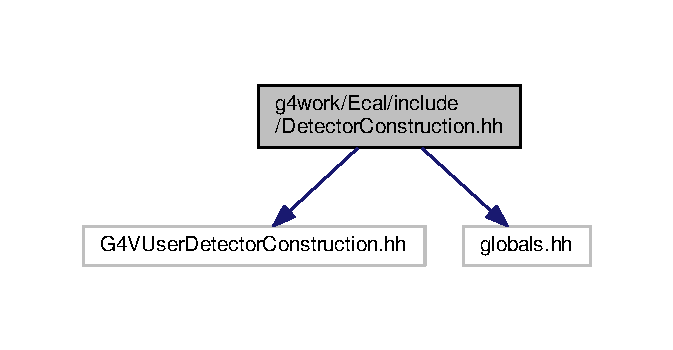
\includegraphics[width=323pt]{_detector_construction_8hh__incl}
\end{center}
\end{figure}
This graph shows which files directly or indirectly include this file\-:\nopagebreak
\begin{figure}[H]
\begin{center}
\leavevmode
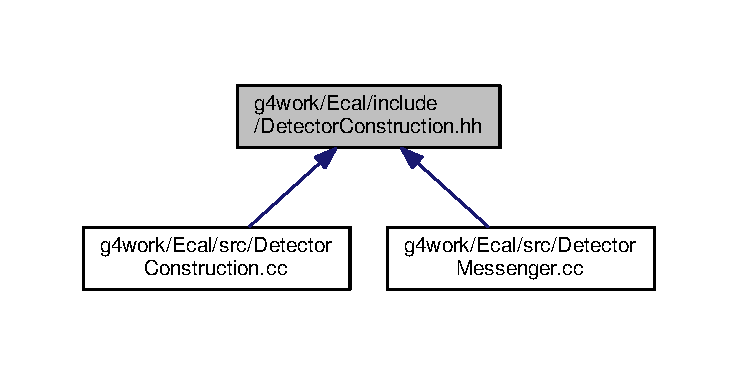
\includegraphics[width=350pt]{_detector_construction_8hh__dep__incl}
\end{center}
\end{figure}
\subsection*{Classes}
\begin{DoxyCompactItemize}
\item 
class \hyperlink{class_detector_construction}{Detector\-Construction}
\end{DoxyCompactItemize}

\hypertarget{_detector_messenger_8hh}{\section{g4work/\-Ecal/include/\-Detector\-Messenger.hh File Reference}
\label{_detector_messenger_8hh}\index{g4work/\-Ecal/include/\-Detector\-Messenger.\-hh@{g4work/\-Ecal/include/\-Detector\-Messenger.\-hh}}
}
{\ttfamily \#include \char`\"{}globals.\-hh\char`\"{}}\\*
{\ttfamily \#include \char`\"{}G4\-U\-Imessenger.\-hh\char`\"{}}\\*
Include dependency graph for Detector\-Messenger.\-hh\-:\nopagebreak
\begin{figure}[H]
\begin{center}
\leavevmode
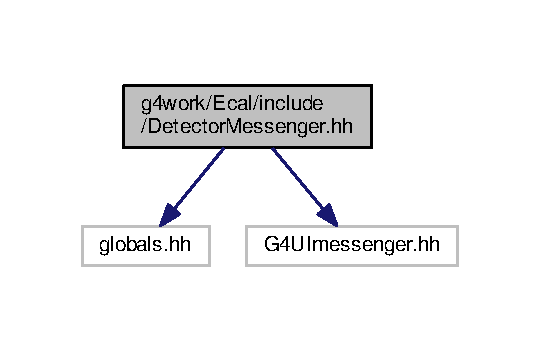
\includegraphics[width=259pt]{_detector_messenger_8hh__incl}
\end{center}
\end{figure}
This graph shows which files directly or indirectly include this file\-:\nopagebreak
\begin{figure}[H]
\begin{center}
\leavevmode
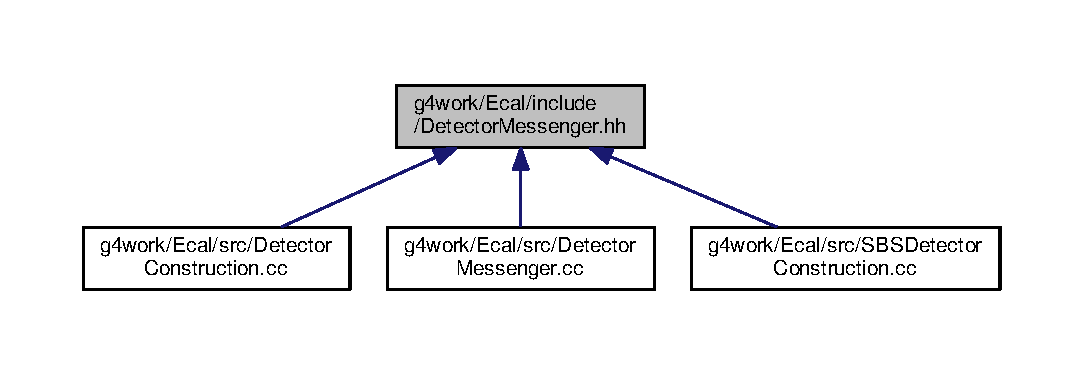
\includegraphics[width=350pt]{_detector_messenger_8hh__dep__incl}
\end{center}
\end{figure}
\subsection*{Classes}
\begin{DoxyCompactItemize}
\item 
class \hyperlink{class_detector_messenger}{Detector\-Messenger}
\end{DoxyCompactItemize}

\hypertarget{_e_cal_analysis_8hh}{\section{g4work/\-Ecal/include/\-E\-Cal\-Analysis.hh File Reference}
\label{_e_cal_analysis_8hh}\index{g4work/\-Ecal/include/\-E\-Cal\-Analysis.\-hh@{g4work/\-Ecal/include/\-E\-Cal\-Analysis.\-hh}}
}
{\ttfamily \#include $<$string$>$}\\*
{\ttfamily \#include $<$iostream$>$}\\*
{\ttfamily \#include $<$sstream$>$}\\*
{\ttfamily \#include \char`\"{}S\-B\-S\-Variables.\-hh\char`\"{}}\\*
{\ttfamily \#include \char`\"{}E\-Cal\-Struct.\-hh\char`\"{}}\\*
{\ttfamily \#include \char`\"{}G4\-Classification\-Of\-New\-Track.\-hh\char`\"{}}\\*
{\ttfamily \#include \char`\"{}G4\-Track\-Status.\-hh\char`\"{}}\\*
{\ttfamily \#include $<$time.\-h$>$}\\*
{\ttfamily \#include \char`\"{}T\-R\-O\-O\-T.\-h\char`\"{}}\\*
{\ttfamily \#include \char`\"{}T\-System.\-h\char`\"{}}\\*
{\ttfamily \#include \char`\"{}T\-File.\-h\char`\"{}}\\*
{\ttfamily \#include \char`\"{}T\-Tree.\-h\char`\"{}}\\*
{\ttfamily \#include \char`\"{}T\-Parameter.\-h\char`\"{}}\\*
{\ttfamily \#include \char`\"{}T\-Random2.\-h\char`\"{}}\\*
Include dependency graph for E\-Cal\-Analysis.\-hh\-:\nopagebreak
\begin{figure}[H]
\begin{center}
\leavevmode
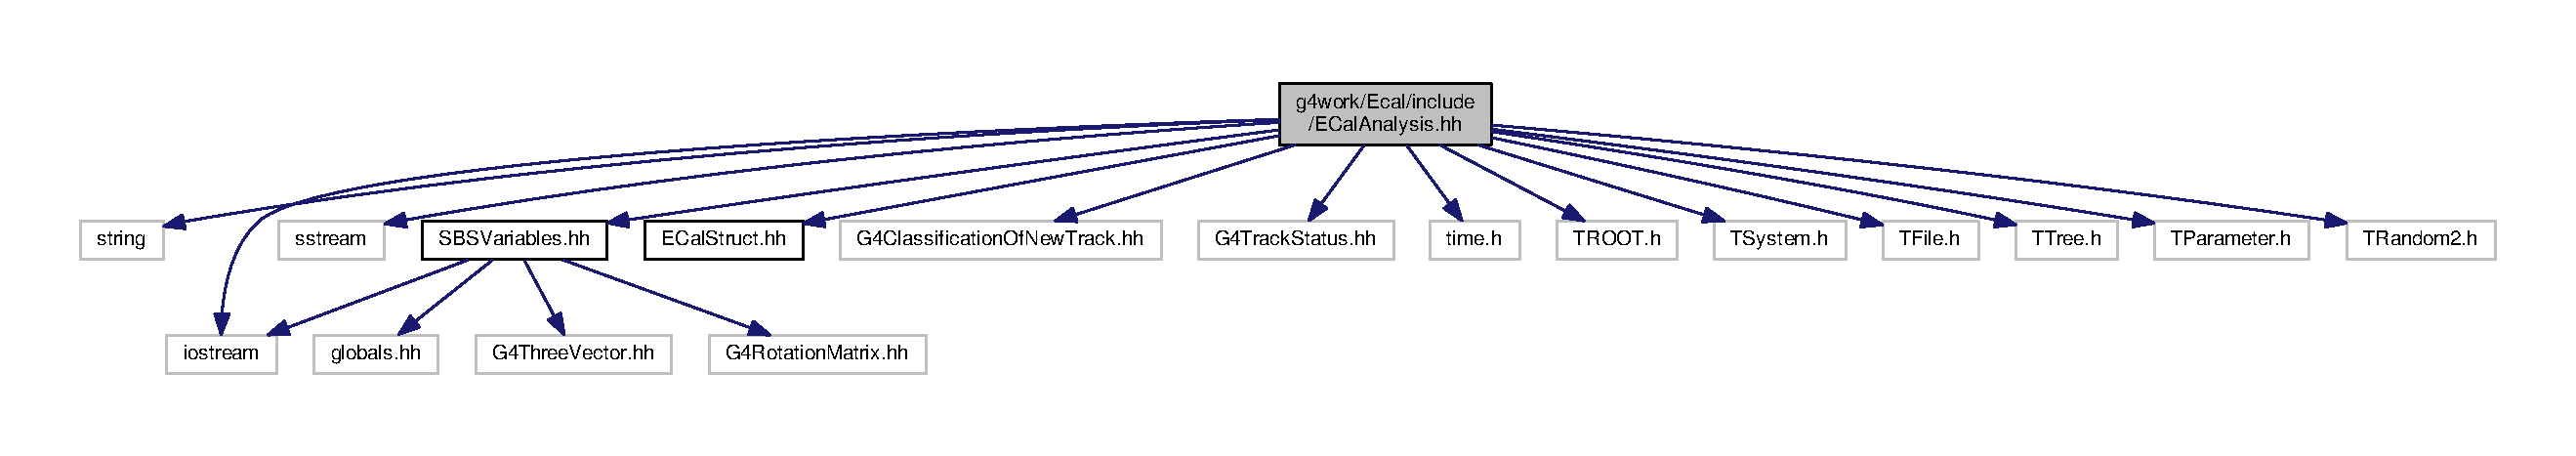
\includegraphics[width=350pt]{_e_cal_analysis_8hh__incl}
\end{center}
\end{figure}
This graph shows which files directly or indirectly include this file\-:\nopagebreak
\begin{figure}[H]
\begin{center}
\leavevmode
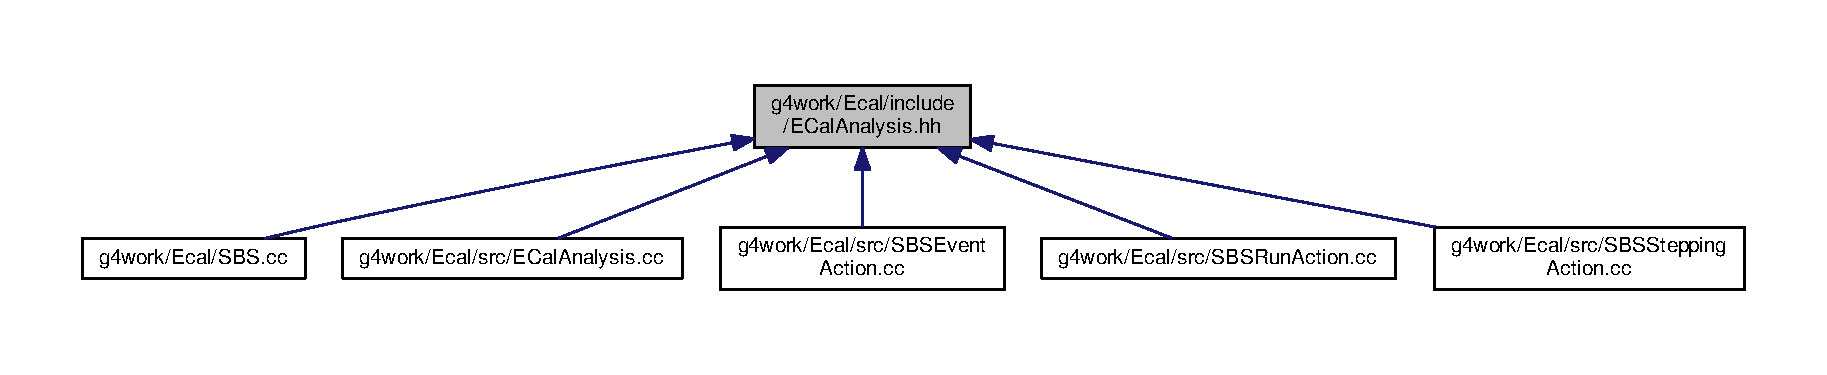
\includegraphics[width=350pt]{_e_cal_analysis_8hh__dep__incl}
\end{center}
\end{figure}
\subsection*{Classes}
\begin{DoxyCompactItemize}
\item 
class \hyperlink{class_e_cal_analysis}{E\-Cal\-Analysis}
\end{DoxyCompactItemize}
\subsection*{Macros}
\begin{DoxyCompactItemize}
\item 
\#define \hyperlink{_e_cal_analysis_8hh_a6800cf6c11218cbba09b5f4338892b52}{G4\-A\-N\-A\-L\-Y\-S\-I\-S\-\_\-\-U\-S\-E\-\_\-\-R\-O\-O\-T}~1
\end{DoxyCompactItemize}


\subsection{Macro Definition Documentation}
\hypertarget{_e_cal_analysis_8hh_a6800cf6c11218cbba09b5f4338892b52}{\index{E\-Cal\-Analysis.\-hh@{E\-Cal\-Analysis.\-hh}!G4\-A\-N\-A\-L\-Y\-S\-I\-S\-\_\-\-U\-S\-E\-\_\-\-R\-O\-O\-T@{G4\-A\-N\-A\-L\-Y\-S\-I\-S\-\_\-\-U\-S\-E\-\_\-\-R\-O\-O\-T}}
\index{G4\-A\-N\-A\-L\-Y\-S\-I\-S\-\_\-\-U\-S\-E\-\_\-\-R\-O\-O\-T@{G4\-A\-N\-A\-L\-Y\-S\-I\-S\-\_\-\-U\-S\-E\-\_\-\-R\-O\-O\-T}!ECalAnalysis.hh@{E\-Cal\-Analysis.\-hh}}
\subsubsection[{G4\-A\-N\-A\-L\-Y\-S\-I\-S\-\_\-\-U\-S\-E\-\_\-\-R\-O\-O\-T}]{\setlength{\rightskip}{0pt plus 5cm}\#define G4\-A\-N\-A\-L\-Y\-S\-I\-S\-\_\-\-U\-S\-E\-\_\-\-R\-O\-O\-T~1}}\label{_e_cal_analysis_8hh_a6800cf6c11218cbba09b5f4338892b52}


Definition at line 59 of file E\-Cal\-Analysis.\-hh.


\hypertarget{_e_cal_detector_construction_8hh}{\section{g4work/\-Ecal/include/\-E\-Cal\-Detector\-Construction.hh File Reference}
\label{_e_cal_detector_construction_8hh}\index{g4work/\-Ecal/include/\-E\-Cal\-Detector\-Construction.\-hh@{g4work/\-Ecal/include/\-E\-Cal\-Detector\-Construction.\-hh}}
}
{\ttfamily \#include \char`\"{}G4\-V\-User\-Detector\-Construction.\-hh\char`\"{}}\\*
{\ttfamily \#include \char`\"{}globals.\-hh\char`\"{}}\\*
Include dependency graph for E\-Cal\-Detector\-Construction.\-hh\-:\nopagebreak
\begin{figure}[H]
\begin{center}
\leavevmode
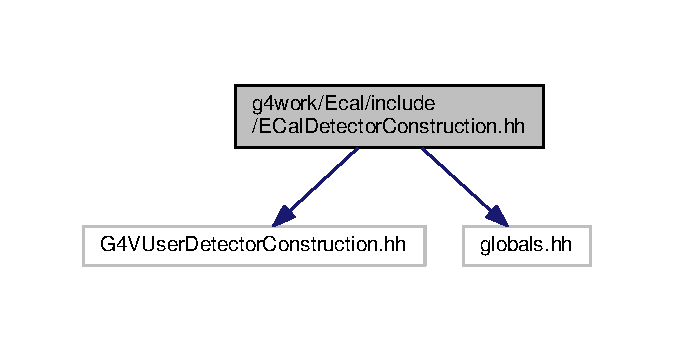
\includegraphics[width=323pt]{_e_cal_detector_construction_8hh__incl}
\end{center}
\end{figure}
This graph shows which files directly or indirectly include this file\-:\nopagebreak
\begin{figure}[H]
\begin{center}
\leavevmode
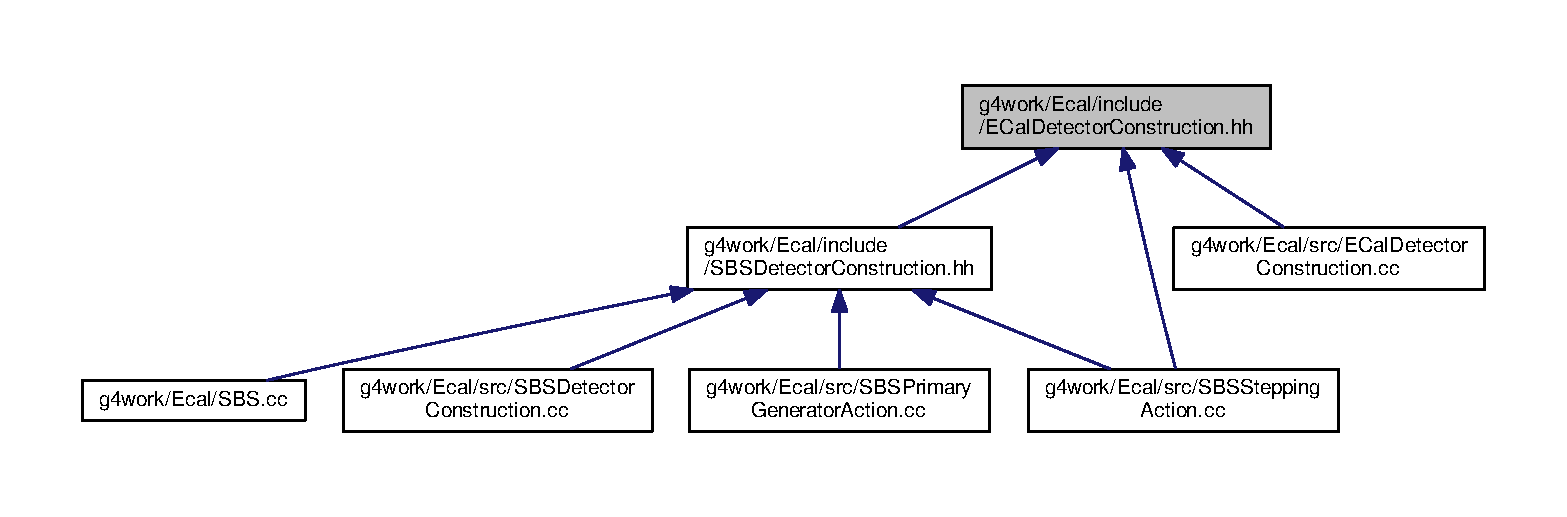
\includegraphics[width=350pt]{_e_cal_detector_construction_8hh__dep__incl}
\end{center}
\end{figure}
\subsection*{Classes}
\begin{DoxyCompactItemize}
\item 
class \hyperlink{class_e_cal_detector_construction}{E\-Cal\-Detector\-Construction}
\end{DoxyCompactItemize}

\hypertarget{_e_cal_struct_8hh}{\section{g4work/\-Ecal/include/\-E\-Cal\-Struct.hh File Reference}
\label{_e_cal_struct_8hh}\index{g4work/\-Ecal/include/\-E\-Cal\-Struct.\-hh@{g4work/\-Ecal/include/\-E\-Cal\-Struct.\-hh}}
}
This graph shows which files directly or indirectly include this file\-:\nopagebreak
\begin{figure}[H]
\begin{center}
\leavevmode
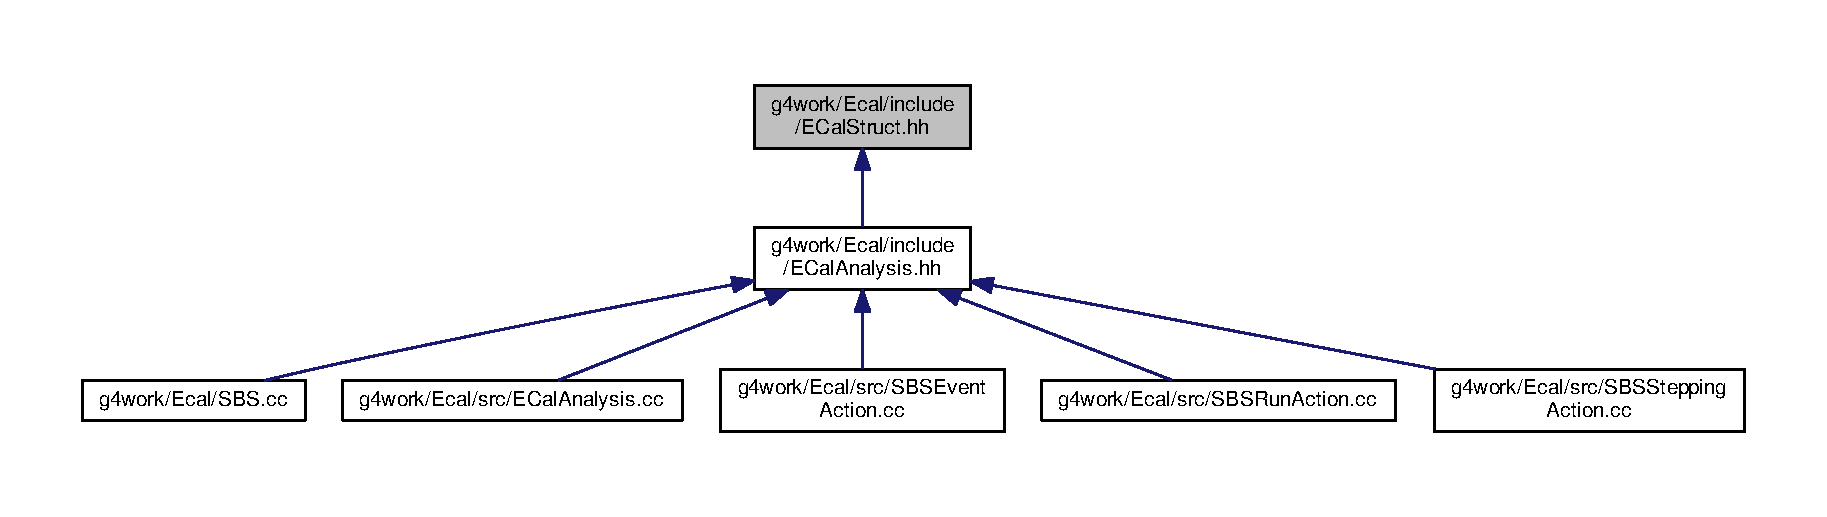
\includegraphics[width=350pt]{_e_cal_struct_8hh__dep__incl}
\end{center}
\end{figure}
\subsection*{Classes}
\begin{DoxyCompactItemize}
\item 
struct \hyperlink{struct_u_thit}{U\-Thit}
\item 
struct \hyperlink{struct_u_t_event}{U\-T\-Event}
\item 
struct \hyperlink{struct_u_t_set}{U\-T\-Set}
\end{DoxyCompactItemize}

\hypertarget{_event_action_messenger_8hh}{\section{g4work/\-Ecal/include/\-Event\-Action\-Messenger.hh File Reference}
\label{_event_action_messenger_8hh}\index{g4work/\-Ecal/include/\-Event\-Action\-Messenger.\-hh@{g4work/\-Ecal/include/\-Event\-Action\-Messenger.\-hh}}
}
{\ttfamily \#include \char`\"{}globals.\-hh\char`\"{}}\\*
{\ttfamily \#include \char`\"{}G4\-U\-Imessenger.\-hh\char`\"{}}\\*
Include dependency graph for Event\-Action\-Messenger.\-hh\-:\nopagebreak
\begin{figure}[H]
\begin{center}
\leavevmode
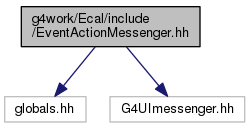
\includegraphics[width=259pt]{_event_action_messenger_8hh__incl}
\end{center}
\end{figure}
This graph shows which files directly or indirectly include this file\-:\nopagebreak
\begin{figure}[H]
\begin{center}
\leavevmode
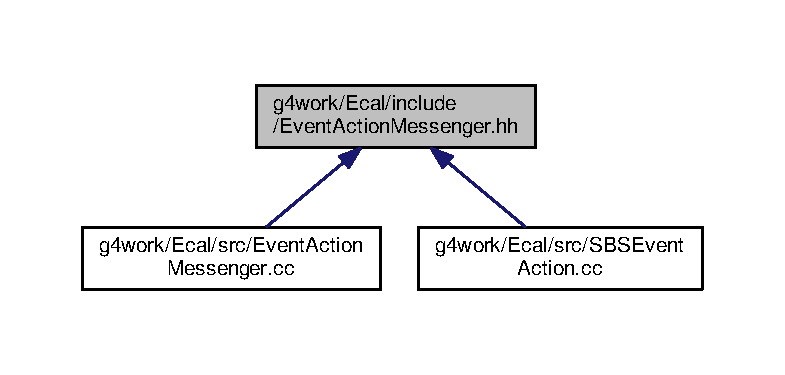
\includegraphics[width=350pt]{_event_action_messenger_8hh__dep__incl}
\end{center}
\end{figure}
\subsection*{Classes}
\begin{DoxyCompactItemize}
\item 
class \hyperlink{class_event_action_messenger}{Event\-Action\-Messenger}
\end{DoxyCompactItemize}

\hypertarget{_physics_list_8hh}{\section{g4work/\-Ecal/include/\-Physics\-List.hh File Reference}
\label{_physics_list_8hh}\index{g4work/\-Ecal/include/\-Physics\-List.\-hh@{g4work/\-Ecal/include/\-Physics\-List.\-hh}}
}
{\ttfamily \#include \char`\"{}G4\-V\-User\-Physics\-List.\-hh\char`\"{}}\\*
{\ttfamily \#include \char`\"{}globals.\-hh\char`\"{}}\\*
Include dependency graph for Physics\-List.\-hh\-:\nopagebreak
\begin{figure}[H]
\begin{center}
\leavevmode
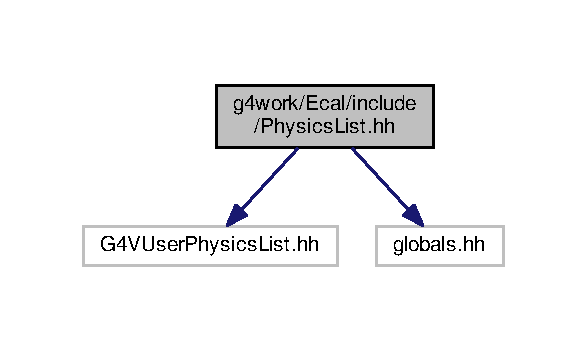
\includegraphics[width=281pt]{_physics_list_8hh__incl}
\end{center}
\end{figure}
This graph shows which files directly or indirectly include this file\-:\nopagebreak
\begin{figure}[H]
\begin{center}
\leavevmode
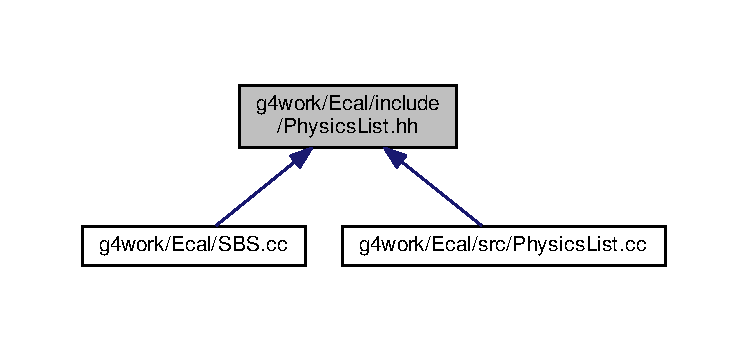
\includegraphics[width=350pt]{_physics_list_8hh__dep__incl}
\end{center}
\end{figure}
\subsection*{Classes}
\begin{DoxyCompactItemize}
\item 
class \hyperlink{class_physics_list}{Physics\-List}
\end{DoxyCompactItemize}

\hypertarget{_primary_generator_messenger_8hh}{\section{g4work/\-Ecal/include/\-Primary\-Generator\-Messenger.hh File Reference}
\label{_primary_generator_messenger_8hh}\index{g4work/\-Ecal/include/\-Primary\-Generator\-Messenger.\-hh@{g4work/\-Ecal/include/\-Primary\-Generator\-Messenger.\-hh}}
}
{\ttfamily \#include \char`\"{}G4\-U\-Imessenger.\-hh\char`\"{}}\\*
{\ttfamily \#include \char`\"{}globals.\-hh\char`\"{}}\\*
Include dependency graph for Primary\-Generator\-Messenger.\-hh\-:\nopagebreak
\begin{figure}[H]
\begin{center}
\leavevmode
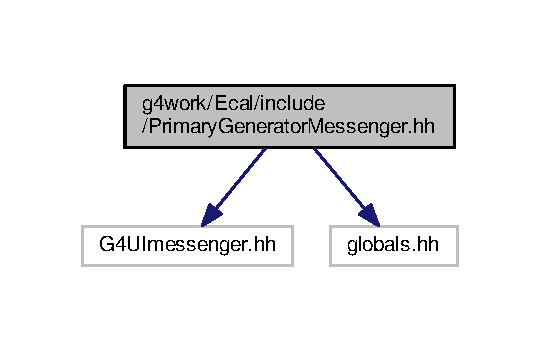
\includegraphics[width=259pt]{_primary_generator_messenger_8hh__incl}
\end{center}
\end{figure}
This graph shows which files directly or indirectly include this file\-:\nopagebreak
\begin{figure}[H]
\begin{center}
\leavevmode
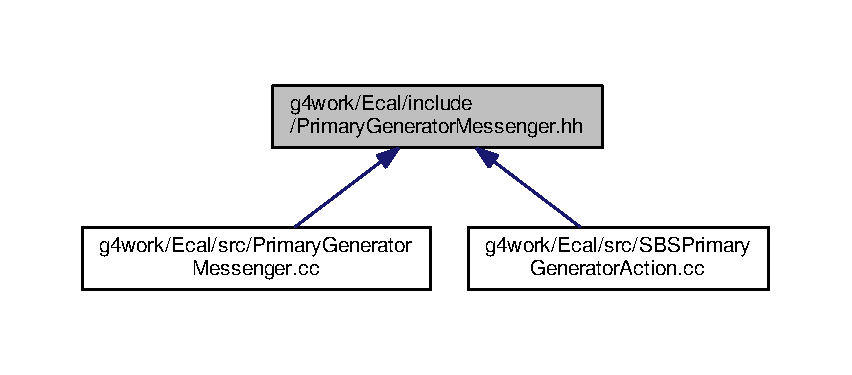
\includegraphics[width=350pt]{_primary_generator_messenger_8hh__dep__incl}
\end{center}
\end{figure}
\subsection*{Classes}
\begin{DoxyCompactItemize}
\item 
class \hyperlink{class_primary_generator_messenger}{Primary\-Generator\-Messenger}
\end{DoxyCompactItemize}

\hypertarget{_s_b_s_constants_8hh}{\section{g4work/\-Ecal/include/\-S\-B\-S\-Constants.hh File Reference}
\label{_s_b_s_constants_8hh}\index{g4work/\-Ecal/include/\-S\-B\-S\-Constants.\-hh@{g4work/\-Ecal/include/\-S\-B\-S\-Constants.\-hh}}
}
{\ttfamily \#include \char`\"{}globals.\-hh\char`\"{}}\\*
{\ttfamily \#include \char`\"{}G4\-Three\-Vector.\-hh\char`\"{}}\\*
Include dependency graph for S\-B\-S\-Constants.\-hh\-:\nopagebreak
\begin{figure}[H]
\begin{center}
\leavevmode
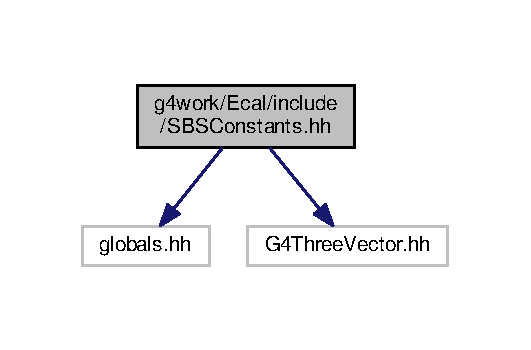
\includegraphics[width=255pt]{_s_b_s_constants_8hh__incl}
\end{center}
\end{figure}
This graph shows which files directly or indirectly include this file\-:\nopagebreak
\begin{figure}[H]
\begin{center}
\leavevmode
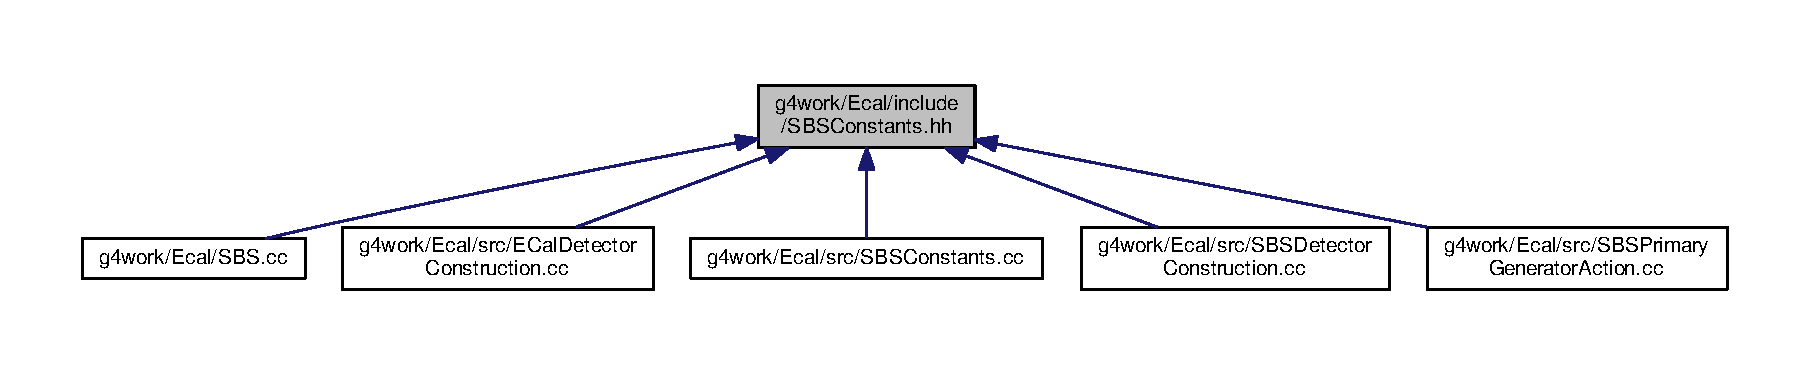
\includegraphics[width=350pt]{_s_b_s_constants_8hh__dep__incl}
\end{center}
\end{figure}
\subsection*{Classes}
\begin{DoxyCompactItemize}
\item 
class \hyperlink{class_s_b_s_constants}{S\-B\-S\-Constants}
\end{DoxyCompactItemize}
\subsection*{Variables}
\begin{DoxyCompactItemize}
\item 
\hyperlink{class_s_b_s_constants}{S\-B\-S\-Constants} $\ast$ \hyperlink{_s_b_s_constants_8hh_a96b2d8ab1753781dd604fbe3a719733c}{Constants}
\end{DoxyCompactItemize}


\subsection{Variable Documentation}
\hypertarget{_s_b_s_constants_8hh_a96b2d8ab1753781dd604fbe3a719733c}{\index{S\-B\-S\-Constants.\-hh@{S\-B\-S\-Constants.\-hh}!Constants@{Constants}}
\index{Constants@{Constants}!SBSConstants.hh@{S\-B\-S\-Constants.\-hh}}
\subsubsection[{Constants}]{\setlength{\rightskip}{0pt plus 5cm}{\bf S\-B\-S\-Constants}$\ast$ Constants}}\label{_s_b_s_constants_8hh_a96b2d8ab1753781dd604fbe3a719733c}


Definition at line 52 of file S\-B\-S\-Constants.\-cc.


\hypertarget{_s_b_s_detector_construction_8hh}{\section{g4work/\-Ecal/include/\-S\-B\-S\-Detector\-Construction.hh File Reference}
\label{_s_b_s_detector_construction_8hh}\index{g4work/\-Ecal/include/\-S\-B\-S\-Detector\-Construction.\-hh@{g4work/\-Ecal/include/\-S\-B\-S\-Detector\-Construction.\-hh}}
}
{\ttfamily \#include \char`\"{}G4\-Run\-Manager.\-hh\char`\"{}}\\*
{\ttfamily \#include \char`\"{}E\-Cal\-Detector\-Construction.\-hh\char`\"{}}\\*
{\ttfamily \#include \char`\"{}G4\-V\-User\-Detector\-Construction.\-hh\char`\"{}}\\*
{\ttfamily \#include \char`\"{}globals.\-hh\char`\"{}}\\*
{\ttfamily \#include $<$C\-L\-H\-E\-P/\-Vector/\-Two\-Vector.\-h$>$}\\*
Include dependency graph for S\-B\-S\-Detector\-Construction.\-hh\-:\nopagebreak
\begin{figure}[H]
\begin{center}
\leavevmode
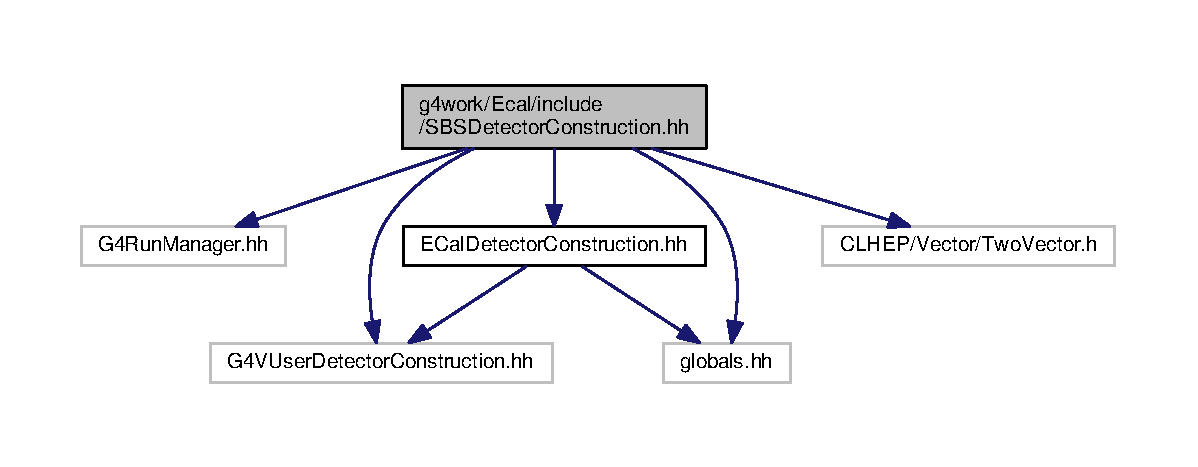
\includegraphics[width=350pt]{_s_b_s_detector_construction_8hh__incl}
\end{center}
\end{figure}
This graph shows which files directly or indirectly include this file\-:\nopagebreak
\begin{figure}[H]
\begin{center}
\leavevmode
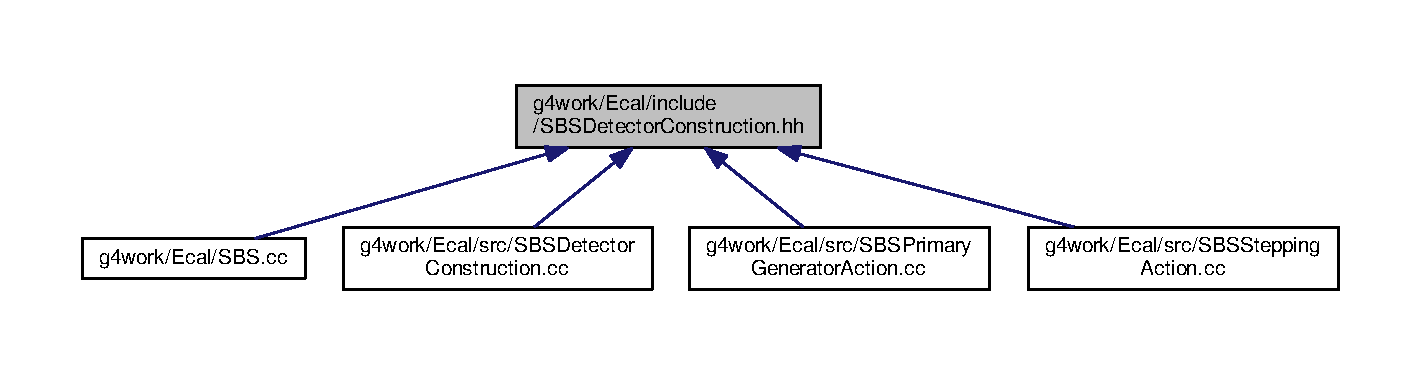
\includegraphics[width=350pt]{_s_b_s_detector_construction_8hh__dep__incl}
\end{center}
\end{figure}
\subsection*{Classes}
\begin{DoxyCompactItemize}
\item 
class \hyperlink{class_s_b_s_detector_construction}{S\-B\-S\-Detector\-Construction}
\end{DoxyCompactItemize}

\hypertarget{_s_b_s_event_action_8hh}{\section{g4work/\-Ecal/include/\-S\-B\-S\-Event\-Action.hh File Reference}
\label{_s_b_s_event_action_8hh}\index{g4work/\-Ecal/include/\-S\-B\-S\-Event\-Action.\-hh@{g4work/\-Ecal/include/\-S\-B\-S\-Event\-Action.\-hh}}
}
{\ttfamily \#include \char`\"{}G4\-User\-Event\-Action.\-hh\char`\"{}}\\*
{\ttfamily \#include \char`\"{}globals.\-hh\char`\"{}}\\*
Include dependency graph for S\-B\-S\-Event\-Action.\-hh\-:\nopagebreak
\begin{figure}[H]
\begin{center}
\leavevmode
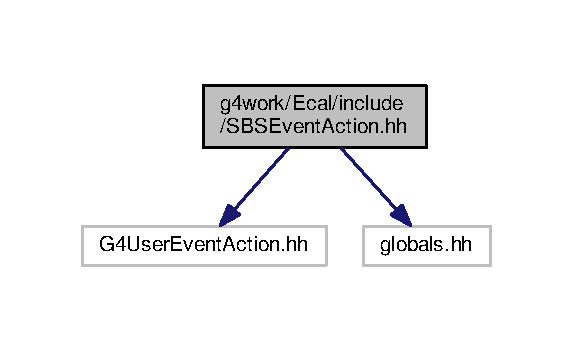
\includegraphics[width=275pt]{_s_b_s_event_action_8hh__incl}
\end{center}
\end{figure}
This graph shows which files directly or indirectly include this file\-:\nopagebreak
\begin{figure}[H]
\begin{center}
\leavevmode
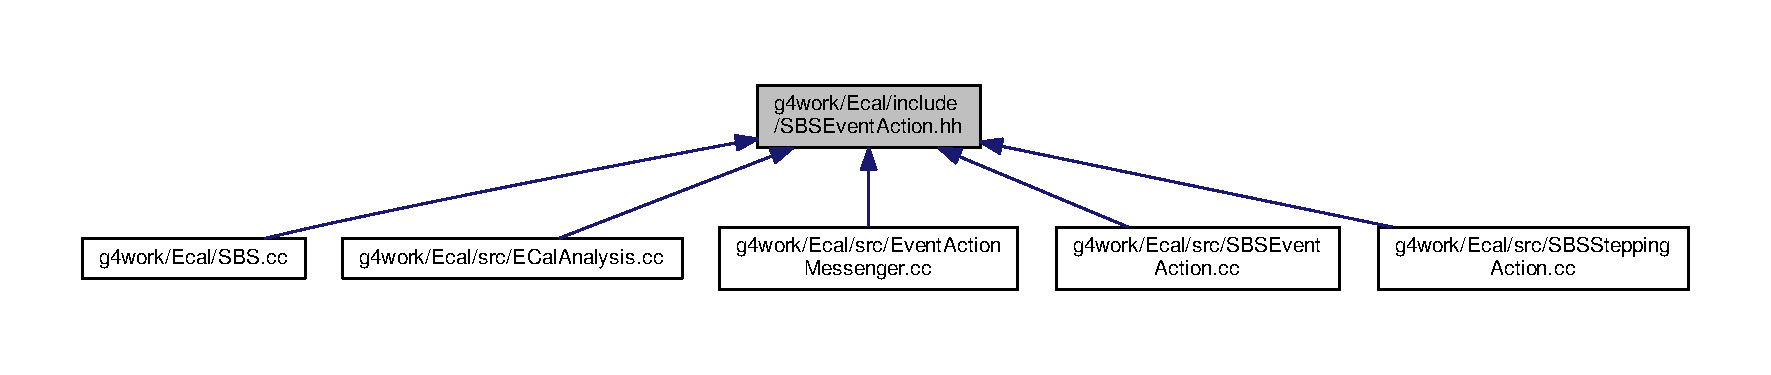
\includegraphics[width=350pt]{_s_b_s_event_action_8hh__dep__incl}
\end{center}
\end{figure}
\subsection*{Classes}
\begin{DoxyCompactItemize}
\item 
class \hyperlink{class_s_b_s_event_action}{S\-B\-S\-Event\-Action}
\end{DoxyCompactItemize}

\hypertarget{_s_b_s_materials_8hh}{\section{g4work/\-Ecal/include/\-S\-B\-S\-Materials.hh File Reference}
\label{_s_b_s_materials_8hh}\index{g4work/\-Ecal/include/\-S\-B\-S\-Materials.\-hh@{g4work/\-Ecal/include/\-S\-B\-S\-Materials.\-hh}}
}
{\ttfamily \#include \char`\"{}globals.\-hh\char`\"{}}\\*
Include dependency graph for S\-B\-S\-Materials.\-hh\-:\nopagebreak
\begin{figure}[H]
\begin{center}
\leavevmode
\includegraphics[width=184pt]{_s_b_s_materials_8hh__incl}
\end{center}
\end{figure}
This graph shows which files directly or indirectly include this file\-:\nopagebreak
\begin{figure}[H]
\begin{center}
\leavevmode
\includegraphics[width=350pt]{_s_b_s_materials_8hh__dep__incl}
\end{center}
\end{figure}
\subsection*{Classes}
\begin{DoxyCompactItemize}
\item 
class \hyperlink{class_s_b_s_materials}{S\-B\-S\-Materials}
\end{DoxyCompactItemize}

\hypertarget{_s_b_s_primary_generator_action_8hh}{\section{g4work/\-Ecal/include/\-S\-B\-S\-Primary\-Generator\-Action.hh File Reference}
\label{_s_b_s_primary_generator_action_8hh}\index{g4work/\-Ecal/include/\-S\-B\-S\-Primary\-Generator\-Action.\-hh@{g4work/\-Ecal/include/\-S\-B\-S\-Primary\-Generator\-Action.\-hh}}
}
{\ttfamily \#include \char`\"{}G4\-V\-User\-Primary\-Generator\-Action.\-hh\char`\"{}}\\*
{\ttfamily \#include \char`\"{}globals.\-hh\char`\"{}}\\*
Include dependency graph for S\-B\-S\-Primary\-Generator\-Action.\-hh\-:\nopagebreak
\begin{figure}[H]
\begin{center}
\leavevmode
\includegraphics[width=333pt]{_s_b_s_primary_generator_action_8hh__incl}
\end{center}
\end{figure}
This graph shows which files directly or indirectly include this file\-:\nopagebreak
\begin{figure}[H]
\begin{center}
\leavevmode
\includegraphics[width=350pt]{_s_b_s_primary_generator_action_8hh__dep__incl}
\end{center}
\end{figure}
\subsection*{Classes}
\begin{DoxyCompactItemize}
\item 
class \hyperlink{class_s_b_s_primary_generator_action}{S\-B\-S\-Primary\-Generator\-Action}
\end{DoxyCompactItemize}

\hypertarget{_s_b_s_run_action_8hh}{\section{g4work/\-Ecal/include/\-S\-B\-S\-Run\-Action.hh File Reference}
\label{_s_b_s_run_action_8hh}\index{g4work/\-Ecal/include/\-S\-B\-S\-Run\-Action.\-hh@{g4work/\-Ecal/include/\-S\-B\-S\-Run\-Action.\-hh}}
}
{\ttfamily \#include \char`\"{}G4\-User\-Run\-Action.\-hh\char`\"{}}\\*
{\ttfamily \#include \char`\"{}globals.\-hh\char`\"{}}\\*
{\ttfamily \#include \char`\"{}S\-B\-S\-Stepping\-Action.\-hh\char`\"{}}\\*
Include dependency graph for S\-B\-S\-Run\-Action.\-hh\-:\nopagebreak
\begin{figure}[H]
\begin{center}
\leavevmode
\includegraphics[width=350pt]{_s_b_s_run_action_8hh__incl}
\end{center}
\end{figure}
This graph shows which files directly or indirectly include this file\-:\nopagebreak
\begin{figure}[H]
\begin{center}
\leavevmode
\includegraphics[width=350pt]{_s_b_s_run_action_8hh__dep__incl}
\end{center}
\end{figure}
\subsection*{Classes}
\begin{DoxyCompactItemize}
\item 
class \hyperlink{class_s_b_s_run_action}{S\-B\-S\-Run\-Action}
\end{DoxyCompactItemize}

\hypertarget{_s_b_s_stepping_action_8hh}{\section{g4work/\-Ecal/include/\-S\-B\-S\-Stepping\-Action.hh File Reference}
\label{_s_b_s_stepping_action_8hh}\index{g4work/\-Ecal/include/\-S\-B\-S\-Stepping\-Action.\-hh@{g4work/\-Ecal/include/\-S\-B\-S\-Stepping\-Action.\-hh}}
}
{\ttfamily \#include \char`\"{}G4\-User\-Stepping\-Action.\-hh\char`\"{}}\\*
{\ttfamily \#include \char`\"{}G4\-Track\-Status.\-hh\char`\"{}}\\*
Include dependency graph for S\-B\-S\-Stepping\-Action.\-hh\-:\nopagebreak
\begin{figure}[H]
\begin{center}
\leavevmode
\includegraphics[width=324pt]{_s_b_s_stepping_action_8hh__incl}
\end{center}
\end{figure}
This graph shows which files directly or indirectly include this file\-:\nopagebreak
\begin{figure}[H]
\begin{center}
\leavevmode
\includegraphics[width=350pt]{_s_b_s_stepping_action_8hh__dep__incl}
\end{center}
\end{figure}
\subsection*{Classes}
\begin{DoxyCompactItemize}
\item 
class \hyperlink{class_s_b_s_stepping_action}{S\-B\-S\-Stepping\-Action}
\end{DoxyCompactItemize}

\hypertarget{_s_b_s_variables_8hh}{\section{g4work/\-Ecal/include/\-S\-B\-S\-Variables.hh File Reference}
\label{_s_b_s_variables_8hh}\index{g4work/\-Ecal/include/\-S\-B\-S\-Variables.\-hh@{g4work/\-Ecal/include/\-S\-B\-S\-Variables.\-hh}}
}
{\ttfamily \#include $<$iostream$>$}\\*
{\ttfamily \#include \char`\"{}globals.\-hh\char`\"{}}\\*
{\ttfamily \#include \char`\"{}G4\-Three\-Vector.\-hh\char`\"{}}\\*
{\ttfamily \#include \char`\"{}G4\-Rotation\-Matrix.\-hh\char`\"{}}\\*
Include dependency graph for S\-B\-S\-Variables.\-hh\-:\nopagebreak
\begin{figure}[H]
\begin{center}
\leavevmode
\includegraphics[width=350pt]{_s_b_s_variables_8hh__incl}
\end{center}
\end{figure}
This graph shows which files directly or indirectly include this file\-:\nopagebreak
\begin{figure}[H]
\begin{center}
\leavevmode
\includegraphics[width=350pt]{_s_b_s_variables_8hh__dep__incl}
\end{center}
\end{figure}
\subsection*{Classes}
\begin{DoxyCompactItemize}
\item 
class \hyperlink{class_s_b_s_variables}{S\-B\-S\-Variables}
\end{DoxyCompactItemize}
\subsection*{Macros}
\begin{DoxyCompactItemize}
\item 
\#define \hyperlink{_s_b_s_variables_8hh_a21d17ff9655f0bbc9bb0faf039bdd525}{No\-Max\-Modules}~3200
\end{DoxyCompactItemize}
\subsection*{Functions}
\begin{DoxyCompactItemize}
\item 
ostream \& \hyperlink{_s_b_s_variables_8hh_a622038ca73b8828dd5c19c780d1de95c}{operator$<$$<$} (ostream \&s, const \hyperlink{class_s_b_s_variables}{S\-B\-S\-Variables} v)
\end{DoxyCompactItemize}
\subsection*{Variables}
\begin{DoxyCompactItemize}
\item 
\hyperlink{class_s_b_s_variables}{S\-B\-S\-Variables} $\ast$ \hyperlink{_s_b_s_variables_8hh_aaa4c7e8ec08cba6569c1ae6ddaa0a388}{Variables}
\end{DoxyCompactItemize}


\subsection{Macro Definition Documentation}
\hypertarget{_s_b_s_variables_8hh_a21d17ff9655f0bbc9bb0faf039bdd525}{\index{S\-B\-S\-Variables.\-hh@{S\-B\-S\-Variables.\-hh}!No\-Max\-Modules@{No\-Max\-Modules}}
\index{No\-Max\-Modules@{No\-Max\-Modules}!SBSVariables.hh@{S\-B\-S\-Variables.\-hh}}
\subsubsection[{No\-Max\-Modules}]{\setlength{\rightskip}{0pt plus 5cm}\#define No\-Max\-Modules~3200}}\label{_s_b_s_variables_8hh_a21d17ff9655f0bbc9bb0faf039bdd525}


Definition at line 13 of file S\-B\-S\-Variables.\-hh.



\subsection{Function Documentation}
\hypertarget{_s_b_s_variables_8hh_a622038ca73b8828dd5c19c780d1de95c}{\index{S\-B\-S\-Variables.\-hh@{S\-B\-S\-Variables.\-hh}!operator$<$$<$@{operator$<$$<$}}
\index{operator$<$$<$@{operator$<$$<$}!SBSVariables.hh@{S\-B\-S\-Variables.\-hh}}
\subsubsection[{operator$<$$<$}]{\setlength{\rightskip}{0pt plus 5cm}ostream\& operator$<$$<$ (
\begin{DoxyParamCaption}
\item[{ostream \&}]{s, }
\item[{const {\bf S\-B\-S\-Variables}}]{v}
\end{DoxyParamCaption}
)}}\label{_s_b_s_variables_8hh_a622038ca73b8828dd5c19c780d1de95c}


Definition at line 274 of file S\-B\-S\-Variables.\-cc.



\subsection{Variable Documentation}
\hypertarget{_s_b_s_variables_8hh_aaa4c7e8ec08cba6569c1ae6ddaa0a388}{\index{S\-B\-S\-Variables.\-hh@{S\-B\-S\-Variables.\-hh}!Variables@{Variables}}
\index{Variables@{Variables}!SBSVariables.hh@{S\-B\-S\-Variables.\-hh}}
\subsubsection[{Variables}]{\setlength{\rightskip}{0pt plus 5cm}{\bf S\-B\-S\-Variables}$\ast$ Variables}}\label{_s_b_s_variables_8hh_aaa4c7e8ec08cba6569c1ae6ddaa0a388}


Definition at line 382 of file S\-B\-S\-Variables.\-cc.


\hypertarget{snprintf_8h}{\section{g4work/\-Ecal/include/snprintf.h File Reference}
\label{snprintf_8h}\index{g4work/\-Ecal/include/snprintf.\-h@{g4work/\-Ecal/include/snprintf.\-h}}
}
{\ttfamily \#include \char`\"{}R\-Config.\-h\char`\"{}}\\*
Include dependency graph for snprintf.\-h\-:\nopagebreak
\begin{figure}[H]
\begin{center}
\leavevmode
\includegraphics[width=184pt]{snprintf_8h__incl}
\end{center}
\end{figure}

\hypertarget{_stepping_verbose_8hh}{\section{g4work/\-Ecal/include/\-Stepping\-Verbose.hh File Reference}
\label{_stepping_verbose_8hh}\index{g4work/\-Ecal/include/\-Stepping\-Verbose.\-hh@{g4work/\-Ecal/include/\-Stepping\-Verbose.\-hh}}
}
{\ttfamily \#include \char`\"{}G4\-Stepping\-Verbose.\-hh\char`\"{}}\\*
Include dependency graph for Stepping\-Verbose.\-hh\-:\nopagebreak
\begin{figure}[H]
\begin{center}
\leavevmode
\includegraphics[width=196pt]{_stepping_verbose_8hh__incl}
\end{center}
\end{figure}
This graph shows which files directly or indirectly include this file\-:\nopagebreak
\begin{figure}[H]
\begin{center}
\leavevmode
\includegraphics[width=333pt]{_stepping_verbose_8hh__dep__incl}
\end{center}
\end{figure}
\subsection*{Classes}
\begin{DoxyCompactItemize}
\item 
class \hyperlink{class_stepping_verbose}{Stepping\-Verbose}
\end{DoxyCompactItemize}

\hypertarget{strlcpy_8h}{\section{g4work/\-Ecal/include/strlcpy.h File Reference}
\label{strlcpy_8h}\index{g4work/\-Ecal/include/strlcpy.\-h@{g4work/\-Ecal/include/strlcpy.\-h}}
}
{\ttfamily \#include \char`\"{}R\-Config.\-h\char`\"{}}\\*
{\ttfamily \#include $<$unistd.\-h$>$}\\*
Include dependency graph for strlcpy.\-h\-:\nopagebreak
\begin{figure}[H]
\begin{center}
\leavevmode
\includegraphics[width=209pt]{strlcpy_8h__incl}
\end{center}
\end{figure}
\subsection*{Functions}
\begin{DoxyCompactItemize}
\item 
size\-\_\-t \hyperlink{strlcpy_8h_aeb79f86261de904967d433c1b5e9a1de}{strlcpy} (char $\ast$dst, const char $\ast$src, size\-\_\-t siz)
\item 
size\-\_\-t \hyperlink{strlcpy_8h_ae85b825a7f3d4dcf136b85949b646a46}{strlcat} (char $\ast$dst, const char $\ast$src, size\-\_\-t siz)
\end{DoxyCompactItemize}


\subsection{Function Documentation}
\hypertarget{strlcpy_8h_ae85b825a7f3d4dcf136b85949b646a46}{\index{strlcpy.\-h@{strlcpy.\-h}!strlcat@{strlcat}}
\index{strlcat@{strlcat}!strlcpy.h@{strlcpy.\-h}}
\subsubsection[{strlcat}]{\setlength{\rightskip}{0pt plus 5cm}size\-\_\-t strlcat (
\begin{DoxyParamCaption}
\item[{char $\ast$}]{dst, }
\item[{const char $\ast$}]{src, }
\item[{size\-\_\-t}]{siz}
\end{DoxyParamCaption}
)}}\label{strlcpy_8h_ae85b825a7f3d4dcf136b85949b646a46}
\hypertarget{strlcpy_8h_aeb79f86261de904967d433c1b5e9a1de}{\index{strlcpy.\-h@{strlcpy.\-h}!strlcpy@{strlcpy}}
\index{strlcpy@{strlcpy}!strlcpy.h@{strlcpy.\-h}}
\subsubsection[{strlcpy}]{\setlength{\rightskip}{0pt plus 5cm}size\-\_\-t strlcpy (
\begin{DoxyParamCaption}
\item[{char $\ast$}]{dst, }
\item[{const char $\ast$}]{src, }
\item[{size\-\_\-t}]{siz}
\end{DoxyParamCaption}
)}}\label{strlcpy_8h_aeb79f86261de904967d433c1b5e9a1de}

\hypertarget{_s_b_s_8cc}{\section{g4work/\-Ecal/\-S\-B\-S.cc File Reference}
\label{_s_b_s_8cc}\index{g4work/\-Ecal/\-S\-B\-S.\-cc@{g4work/\-Ecal/\-S\-B\-S.\-cc}}
}
{\ttfamily \#include \char`\"{}G4\-Run\-Manager.\-hh\char`\"{}}\\*
{\ttfamily \#include \char`\"{}G4\-U\-Imanager.\-hh\char`\"{}}\\*
{\ttfamily \#include \char`\"{}Randomize.\-hh\char`\"{}}\\*
{\ttfamily \#include \char`\"{}S\-B\-S\-Constants.\-hh\char`\"{}}\\*
{\ttfamily \#include \char`\"{}S\-B\-S\-Variables.\-hh\char`\"{}}\\*
{\ttfamily \#include \char`\"{}S\-B\-S\-Detector\-Construction.\-hh\char`\"{}}\\*
{\ttfamily \#include \char`\"{}S\-B\-S\-Primary\-Generator\-Action.\-hh\char`\"{}}\\*
{\ttfamily \#include \char`\"{}S\-B\-S\-Event\-Action.\-hh\char`\"{}}\\*
{\ttfamily \#include \char`\"{}S\-B\-S\-Run\-Action.\-hh\char`\"{}}\\*
{\ttfamily \#include \char`\"{}S\-B\-S\-Stepping\-Action.\-hh\char`\"{}}\\*
{\ttfamily \#include \char`\"{}E\-Cal\-Analysis.\-hh\char`\"{}}\\*
{\ttfamily \#include \char`\"{}Physics\-List.\-hh\char`\"{}}\\*
{\ttfamily \#include \char`\"{}Stepping\-Verbose.\-hh\char`\"{}}\\*
Include dependency graph for S\-B\-S.\-cc\-:\nopagebreak
\begin{figure}[H]
\begin{center}
\leavevmode
\includegraphics[width=350pt]{_s_b_s_8cc__incl}
\end{center}
\end{figure}
\subsection*{Functions}
\begin{DoxyCompactItemize}
\item 
int \hyperlink{_s_b_s_8cc_a3c04138a5bfe5d72780bb7e82a18e627}{main} (int argc, char $\ast$$\ast$argv)
\end{DoxyCompactItemize}


\subsection{Function Documentation}
\hypertarget{_s_b_s_8cc_a3c04138a5bfe5d72780bb7e82a18e627}{\index{S\-B\-S.\-cc@{S\-B\-S.\-cc}!main@{main}}
\index{main@{main}!SBS.cc@{S\-B\-S.\-cc}}
\subsubsection[{main}]{\setlength{\rightskip}{0pt plus 5cm}int main (
\begin{DoxyParamCaption}
\item[{int}]{argc, }
\item[{char $\ast$$\ast$}]{argv}
\end{DoxyParamCaption}
)}}\label{_s_b_s_8cc_a3c04138a5bfe5d72780bb7e82a18e627}


Definition at line 63 of file S\-B\-S.\-cc.



Here is the call graph for this function\-:\nopagebreak
\begin{figure}[H]
\begin{center}
\leavevmode
\includegraphics[width=298pt]{_s_b_s_8cc_a3c04138a5bfe5d72780bb7e82a18e627_cgraph}
\end{center}
\end{figure}



\hypertarget{_detector_construction_8cc}{\section{g4work/\-Ecal/src/\-Detector\-Construction.cc File Reference}
\label{_detector_construction_8cc}\index{g4work/\-Ecal/src/\-Detector\-Construction.\-cc@{g4work/\-Ecal/src/\-Detector\-Construction.\-cc}}
}
{\ttfamily \#include \char`\"{}Detector\-Construction.\-hh\char`\"{}}\\*
{\ttfamily \#include \char`\"{}Detector\-Messenger.\-hh\char`\"{}}\\*
{\ttfamily \#include \char`\"{}G4\-Material.\-hh\char`\"{}}\\*
{\ttfamily \#include \char`\"{}G4\-Nist\-Manager.\-hh\char`\"{}}\\*
{\ttfamily \#include \char`\"{}G4\-Box.\-hh\char`\"{}}\\*
{\ttfamily \#include \char`\"{}G4\-Logical\-Volume.\-hh\char`\"{}}\\*
{\ttfamily \#include \char`\"{}G4\-P\-V\-Placement.\-hh\char`\"{}}\\*
{\ttfamily \#include \char`\"{}G4\-P\-V\-Replica.\-hh\char`\"{}}\\*
{\ttfamily \#include \char`\"{}G4\-Uniform\-Mag\-Field.\-hh\char`\"{}}\\*
{\ttfamily \#include \char`\"{}G4\-Geometry\-Manager.\-hh\char`\"{}}\\*
{\ttfamily \#include \char`\"{}G4\-Physical\-Volume\-Store.\-hh\char`\"{}}\\*
{\ttfamily \#include \char`\"{}G4\-Logical\-Volume\-Store.\-hh\char`\"{}}\\*
{\ttfamily \#include \char`\"{}G4\-Solid\-Store.\-hh\char`\"{}}\\*
{\ttfamily \#include \char`\"{}G4\-Vis\-Attributes.\-hh\char`\"{}}\\*
{\ttfamily \#include \char`\"{}G4\-Colour.\-hh\char`\"{}}\\*
{\ttfamily \#include \char`\"{}G4\-Field\-Manager.\-hh\char`\"{}}\\*
{\ttfamily \#include \char`\"{}G4\-Transportation\-Manager.\-hh\char`\"{}}\\*
{\ttfamily \#include \char`\"{}G4\-Run\-Manager.\-hh\char`\"{}}\\*
Include dependency graph for Detector\-Construction.\-cc\-:\nopagebreak
\begin{figure}[H]
\begin{center}
\leavevmode
\includegraphics[width=350pt]{_detector_construction_8cc__incl}
\end{center}
\end{figure}

\hypertarget{_detector_messenger_8cc}{\section{g4work/\-Ecal/src/\-Detector\-Messenger.cc File Reference}
\label{_detector_messenger_8cc}\index{g4work/\-Ecal/src/\-Detector\-Messenger.\-cc@{g4work/\-Ecal/src/\-Detector\-Messenger.\-cc}}
}
{\ttfamily \#include \char`\"{}Detector\-Messenger.\-hh\char`\"{}}\\*
{\ttfamily \#include \char`\"{}Detector\-Construction.\-hh\char`\"{}}\\*
{\ttfamily \#include \char`\"{}G4\-U\-Idirectory.\-hh\char`\"{}}\\*
{\ttfamily \#include \char`\"{}G4\-U\-Icmd\-With\-A\-String.\-hh\char`\"{}}\\*
{\ttfamily \#include \char`\"{}G4\-U\-Icmd\-With\-An\-Integer.\-hh\char`\"{}}\\*
{\ttfamily \#include \char`\"{}G4\-U\-Icmd\-With\-A\-Double\-And\-Unit.\-hh\char`\"{}}\\*
{\ttfamily \#include \char`\"{}G4\-U\-Icmd\-Without\-Parameter.\-hh\char`\"{}}\\*
Include dependency graph for Detector\-Messenger.\-cc\-:\nopagebreak
\begin{figure}[H]
\begin{center}
\leavevmode
\includegraphics[width=350pt]{_detector_messenger_8cc__incl}
\end{center}
\end{figure}

\hypertarget{_e_cal_analysis_8cc}{\section{g4work/\-Ecal/src/\-E\-Cal\-Analysis.cc File Reference}
\label{_e_cal_analysis_8cc}\index{g4work/\-Ecal/src/\-E\-Cal\-Analysis.\-cc@{g4work/\-Ecal/src/\-E\-Cal\-Analysis.\-cc}}
}
{\ttfamily \#include $<$time.\-h$>$}\\*
{\ttfamily \#include \char`\"{}E\-Cal\-Analysis.\-hh\char`\"{}}\\*
{\ttfamily \#include \char`\"{}S\-B\-S\-Event\-Action.\-hh\char`\"{}}\\*
{\ttfamily \#include \char`\"{}G4ios.\-hh\char`\"{}}\\*
{\ttfamily \#include \char`\"{}G4\-Units\-Table.\-hh\char`\"{}}\\*
{\ttfamily \#include \char`\"{}G4\-V\-Physical\-Volume.\-hh\char`\"{}}\\*
{\ttfamily \#include \char`\"{}G4\-Event.\-hh\char`\"{}}\\*
{\ttfamily \#include \char`\"{}G4\-Run.\-hh\char`\"{}}\\*
{\ttfamily \#include \char`\"{}G4\-Track.\-hh\char`\"{}}\\*
{\ttfamily \#include \char`\"{}G4\-Classification\-Of\-New\-Track.\-hh\char`\"{}}\\*
{\ttfamily \#include \char`\"{}G4\-Track\-Status.\-hh\char`\"{}}\\*
{\ttfamily \#include \char`\"{}G4\-Step.\-hh\char`\"{}}\\*
{\ttfamily \#include \char`\"{}G4\-Types.\-hh\char`\"{}}\\*
{\ttfamily \#include \char`\"{}G4\-U\-Imanager.\-hh\char`\"{}}\\*
{\ttfamily \#include \char`\"{}G4\-Material\-Cuts\-Couple.\-hh\char`\"{}}\\*
{\ttfamily \#include \char`\"{}G4\-Material.\-hh\char`\"{}}\\*
Include dependency graph for E\-Cal\-Analysis.\-cc\-:\nopagebreak
\begin{figure}[H]
\begin{center}
\leavevmode
\includegraphics[width=350pt]{_e_cal_analysis_8cc__incl}
\end{center}
\end{figure}

\hypertarget{_e_cal_detector_construction_8cc}{\section{g4work/\-Ecal/src/\-E\-Cal\-Detector\-Construction.cc File Reference}
\label{_e_cal_detector_construction_8cc}\index{g4work/\-Ecal/src/\-E\-Cal\-Detector\-Construction.\-cc@{g4work/\-Ecal/src/\-E\-Cal\-Detector\-Construction.\-cc}}
}
{\ttfamily \#include \char`\"{}G4\-Material.\-hh\char`\"{}}\\*
{\ttfamily \#include \char`\"{}G4\-Nist\-Manager.\-hh\char`\"{}}\\*
{\ttfamily \#include \char`\"{}G4\-Subtraction\-Solid.\-hh\char`\"{}}\\*
{\ttfamily \#include \char`\"{}G4\-Box.\-hh\char`\"{}}\\*
{\ttfamily \#include \char`\"{}G4\-Tubs.\-hh\char`\"{}}\\*
{\ttfamily \#include \char`\"{}G4\-Logical\-Volume.\-hh\char`\"{}}\\*
{\ttfamily \#include \char`\"{}G4\-P\-V\-Placement.\-hh\char`\"{}}\\*
{\ttfamily \#include \char`\"{}G4\-P\-V\-Replica.\-hh\char`\"{}}\\*
{\ttfamily \#include \char`\"{}G4\-Uniform\-Mag\-Field.\-hh\char`\"{}}\\*
{\ttfamily \#include \char`\"{}G4\-Geometry\-Manager.\-hh\char`\"{}}\\*
{\ttfamily \#include \char`\"{}G4\-Physical\-Volume\-Store.\-hh\char`\"{}}\\*
{\ttfamily \#include \char`\"{}G4\-Logical\-Volume\-Store.\-hh\char`\"{}}\\*
{\ttfamily \#include \char`\"{}G4\-Solid\-Store.\-hh\char`\"{}}\\*
{\ttfamily \#include \char`\"{}G4\-Vis\-Attributes.\-hh\char`\"{}}\\*
{\ttfamily \#include \char`\"{}G4\-Colour.\-hh\char`\"{}}\\*
{\ttfamily \#include \char`\"{}S\-B\-S\-Variables.\-hh\char`\"{}}\\*
{\ttfamily \#include \char`\"{}S\-B\-S\-Constants.\-hh\char`\"{}}\\*
{\ttfamily \#include \char`\"{}E\-Cal\-Detector\-Construction.\-hh\char`\"{}}\\*
{\ttfamily \#include \char`\"{}S\-B\-S\-Materials.\-hh\char`\"{}}\\*
Include dependency graph for E\-Cal\-Detector\-Construction.\-cc\-:\nopagebreak
\begin{figure}[H]
\begin{center}
\leavevmode
\includegraphics[width=350pt]{_e_cal_detector_construction_8cc__incl}
\end{center}
\end{figure}

\hypertarget{_event_action_messenger_8cc}{\section{g4work/\-Ecal/src/\-Event\-Action\-Messenger.cc File Reference}
\label{_event_action_messenger_8cc}\index{g4work/\-Ecal/src/\-Event\-Action\-Messenger.\-cc@{g4work/\-Ecal/src/\-Event\-Action\-Messenger.\-cc}}
}
{\ttfamily \#include \char`\"{}Event\-Action\-Messenger.\-hh\char`\"{}}\\*
{\ttfamily \#include \char`\"{}S\-B\-S\-Event\-Action.\-hh\char`\"{}}\\*
{\ttfamily \#include \char`\"{}G4\-U\-Idirectory.\-hh\char`\"{}}\\*
{\ttfamily \#include \char`\"{}G4\-U\-Icmd\-With\-An\-Integer.\-hh\char`\"{}}\\*
{\ttfamily \#include \char`\"{}globals.\-hh\char`\"{}}\\*
Include dependency graph for Event\-Action\-Messenger.\-cc\-:\nopagebreak
\begin{figure}[H]
\begin{center}
\leavevmode
\includegraphics[width=350pt]{_event_action_messenger_8cc__incl}
\end{center}
\end{figure}

\hypertarget{_physics_list_8cc}{\section{g4work/\-Ecal/src/\-Physics\-List.cc File Reference}
\label{_physics_list_8cc}\index{g4work/\-Ecal/src/\-Physics\-List.\-cc@{g4work/\-Ecal/src/\-Physics\-List.\-cc}}
}
{\ttfamily \#include \char`\"{}Physics\-List.\-hh\char`\"{}}\\*
{\ttfamily \#include \char`\"{}G4\-Process\-Manager.\-hh\char`\"{}}\\*
{\ttfamily \#include \char`\"{}G4\-Boson\-Constructor.\-hh\char`\"{}}\\*
{\ttfamily \#include \char`\"{}G4\-Lepton\-Constructor.\-hh\char`\"{}}\\*
{\ttfamily \#include \char`\"{}G4\-Meson\-Constructor.\-hh\char`\"{}}\\*
{\ttfamily \#include \char`\"{}G4\-Baryon\-Constructor.\-hh\char`\"{}}\\*
{\ttfamily \#include \char`\"{}G4\-Ion\-Constructor.\-hh\char`\"{}}\\*
{\ttfamily \#include \char`\"{}G4\-Physics\-List\-Helper.\-hh\char`\"{}}\\*
{\ttfamily \#include \char`\"{}G4\-Compton\-Scattering.\-hh\char`\"{}}\\*
{\ttfamily \#include \char`\"{}G4\-Gamma\-Conversion.\-hh\char`\"{}}\\*
{\ttfamily \#include \char`\"{}G4\-Photo\-Electric\-Effect.\-hh\char`\"{}}\\*
{\ttfamily \#include \char`\"{}G4e\-Multiple\-Scattering.\-hh\char`\"{}}\\*
{\ttfamily \#include \char`\"{}G4e\-Ionisation.\-hh\char`\"{}}\\*
{\ttfamily \#include \char`\"{}G4e\-Bremsstrahlung.\-hh\char`\"{}}\\*
{\ttfamily \#include \char`\"{}G4eplus\-Annihilation.\-hh\char`\"{}}\\*
{\ttfamily \#include \char`\"{}G4\-Mu\-Multiple\-Scattering.\-hh\char`\"{}}\\*
{\ttfamily \#include \char`\"{}G4\-Mu\-Ionisation.\-hh\char`\"{}}\\*
{\ttfamily \#include \char`\"{}G4\-Mu\-Bremsstrahlung.\-hh\char`\"{}}\\*
{\ttfamily \#include \char`\"{}G4\-Mu\-Pair\-Production.\-hh\char`\"{}}\\*
{\ttfamily \#include \char`\"{}G4h\-Multiple\-Scattering.\-hh\char`\"{}}\\*
{\ttfamily \#include \char`\"{}G4h\-Ionisation.\-hh\char`\"{}}\\*
{\ttfamily \#include \char`\"{}G4h\-Bremsstrahlung.\-hh\char`\"{}}\\*
{\ttfamily \#include \char`\"{}G4h\-Pair\-Production.\-hh\char`\"{}}\\*
{\ttfamily \#include \char`\"{}G4ion\-Ionisation.\-hh\char`\"{}}\\*
{\ttfamily \#include \char`\"{}G4\-Decay.\-hh\char`\"{}}\\*
Include dependency graph for Physics\-List.\-cc\-:\nopagebreak
\begin{figure}[H]
\begin{center}
\leavevmode
\includegraphics[width=350pt]{_physics_list_8cc__incl}
\end{center}
\end{figure}

\hypertarget{_primary_generator_messenger_8cc}{\section{g4work/\-Ecal/src/\-Primary\-Generator\-Messenger.cc File Reference}
\label{_primary_generator_messenger_8cc}\index{g4work/\-Ecal/src/\-Primary\-Generator\-Messenger.\-cc@{g4work/\-Ecal/src/\-Primary\-Generator\-Messenger.\-cc}}
}
{\ttfamily \#include \char`\"{}Primary\-Generator\-Messenger.\-hh\char`\"{}}\\*
{\ttfamily \#include \char`\"{}S\-B\-S\-Primary\-Generator\-Action.\-hh\char`\"{}}\\*
{\ttfamily \#include \char`\"{}G4\-U\-Idirectory.\-hh\char`\"{}}\\*
{\ttfamily \#include \char`\"{}G4\-U\-Icmd\-With\-A\-String.\-hh\char`\"{}}\\*
Include dependency graph for Primary\-Generator\-Messenger.\-cc\-:\nopagebreak
\begin{figure}[H]
\begin{center}
\leavevmode
\includegraphics[width=350pt]{_primary_generator_messenger_8cc__incl}
\end{center}
\end{figure}

\hypertarget{_s_b_s_constants_8cc}{\section{g4work/\-Ecal/src/\-S\-B\-S\-Constants.cc File Reference}
\label{_s_b_s_constants_8cc}\index{g4work/\-Ecal/src/\-S\-B\-S\-Constants.\-cc@{g4work/\-Ecal/src/\-S\-B\-S\-Constants.\-cc}}
}
{\ttfamily \#include \char`\"{}S\-B\-S\-Variables.\-hh\char`\"{}}\\*
{\ttfamily \#include \char`\"{}S\-B\-S\-Constants.\-hh\char`\"{}}\\*
Include dependency graph for S\-B\-S\-Constants.\-cc\-:\nopagebreak
\begin{figure}[H]
\begin{center}
\leavevmode
\includegraphics[width=350pt]{_s_b_s_constants_8cc__incl}
\end{center}
\end{figure}
\subsection*{Variables}
\begin{DoxyCompactItemize}
\item 
\hyperlink{class_s_b_s_constants}{S\-B\-S\-Constants} $\ast$ \hyperlink{_s_b_s_constants_8cc_a96b2d8ab1753781dd604fbe3a719733c}{Constants} = N\-U\-L\-L
\end{DoxyCompactItemize}


\subsection{Variable Documentation}
\hypertarget{_s_b_s_constants_8cc_a96b2d8ab1753781dd604fbe3a719733c}{\index{S\-B\-S\-Constants.\-cc@{S\-B\-S\-Constants.\-cc}!Constants@{Constants}}
\index{Constants@{Constants}!SBSConstants.cc@{S\-B\-S\-Constants.\-cc}}
\subsubsection[{Constants}]{\setlength{\rightskip}{0pt plus 5cm}{\bf S\-B\-S\-Constants}$\ast$ Constants = N\-U\-L\-L}}\label{_s_b_s_constants_8cc_a96b2d8ab1753781dd604fbe3a719733c}


Definition at line 52 of file S\-B\-S\-Constants.\-cc.


\hypertarget{_s_b_s_detector_construction_8cc}{\section{g4work/\-Ecal/src/\-S\-B\-S\-Detector\-Construction.cc File Reference}
\label{_s_b_s_detector_construction_8cc}\index{g4work/\-Ecal/src/\-S\-B\-S\-Detector\-Construction.\-cc@{g4work/\-Ecal/src/\-S\-B\-S\-Detector\-Construction.\-cc}}
}
{\ttfamily \#include \char`\"{}G4\-Material.\-hh\char`\"{}}\\*
{\ttfamily \#include \char`\"{}G4\-Nist\-Manager.\-hh\char`\"{}}\\*
{\ttfamily \#include \char`\"{}G4\-Box.\-hh\char`\"{}}\\*
{\ttfamily \#include \char`\"{}G4\-Logical\-Volume.\-hh\char`\"{}}\\*
{\ttfamily \#include \char`\"{}G4\-P\-V\-Placement.\-hh\char`\"{}}\\*
{\ttfamily \#include \char`\"{}G4\-P\-V\-Replica.\-hh\char`\"{}}\\*
{\ttfamily \#include \char`\"{}G4\-Uniform\-Mag\-Field.\-hh\char`\"{}}\\*
{\ttfamily \#include \char`\"{}G4\-Geometry\-Manager.\-hh\char`\"{}}\\*
{\ttfamily \#include \char`\"{}G4\-Physical\-Volume\-Store.\-hh\char`\"{}}\\*
{\ttfamily \#include \char`\"{}G4\-Logical\-Volume\-Store.\-hh\char`\"{}}\\*
{\ttfamily \#include \char`\"{}G4\-Solid\-Store.\-hh\char`\"{}}\\*
{\ttfamily \#include \char`\"{}G4\-Vis\-Attributes.\-hh\char`\"{}}\\*
{\ttfamily \#include \char`\"{}G4\-Colour.\-hh\char`\"{}}\\*
{\ttfamily \#include \char`\"{}S\-B\-S\-Materials.\-hh\char`\"{}}\\*
{\ttfamily \#include \char`\"{}S\-B\-S\-Detector\-Construction.\-hh\char`\"{}}\\*
{\ttfamily \#include \char`\"{}Detector\-Messenger.\-hh\char`\"{}}\\*
{\ttfamily \#include \char`\"{}S\-B\-S\-Constants.\-hh\char`\"{}}\\*
{\ttfamily \#include \char`\"{}G4\-Field\-Manager.\-hh\char`\"{}}\\*
{\ttfamily \#include \char`\"{}G4\-Transportation\-Manager.\-hh\char`\"{}}\\*
{\ttfamily \#include \char`\"{}G4\-Run\-Manager.\-hh\char`\"{}}\\*
Include dependency graph for S\-B\-S\-Detector\-Construction.\-cc\-:\nopagebreak
\begin{figure}[H]
\begin{center}
\leavevmode
\includegraphics[width=350pt]{_s_b_s_detector_construction_8cc__incl}
\end{center}
\end{figure}

\hypertarget{_s_b_s_event_action_8cc}{\section{g4work/\-Ecal/src/\-S\-B\-S\-Event\-Action.cc File Reference}
\label{_s_b_s_event_action_8cc}\index{g4work/\-Ecal/src/\-S\-B\-S\-Event\-Action.\-cc@{g4work/\-Ecal/src/\-S\-B\-S\-Event\-Action.\-cc}}
}
{\ttfamily \#include \char`\"{}S\-B\-S\-Event\-Action.\-hh\char`\"{}}\\*
{\ttfamily \#include \char`\"{}E\-Cal\-Analysis.\-hh\char`\"{}}\\*
{\ttfamily \#include \char`\"{}S\-B\-S\-Run\-Action.\-hh\char`\"{}}\\*
{\ttfamily \#include \char`\"{}Event\-Action\-Messenger.\-hh\char`\"{}}\\*
{\ttfamily \#include \char`\"{}G4\-Run\-Manager.\-hh\char`\"{}}\\*
{\ttfamily \#include \char`\"{}G4\-Event.\-hh\char`\"{}}\\*
{\ttfamily \#include \char`\"{}G4\-Units\-Table.\-hh\char`\"{}}\\*
{\ttfamily \#include \char`\"{}Randomize.\-hh\char`\"{}}\\*
{\ttfamily \#include $<$iomanip$>$}\\*
Include dependency graph for S\-B\-S\-Event\-Action.\-cc\-:\nopagebreak
\begin{figure}[H]
\begin{center}
\leavevmode
\includegraphics[width=350pt]{_s_b_s_event_action_8cc__incl}
\end{center}
\end{figure}

\hypertarget{_s_b_s_materials_8cc}{\section{g4work/\-Ecal/src/\-S\-B\-S\-Materials.cc File Reference}
\label{_s_b_s_materials_8cc}\index{g4work/\-Ecal/src/\-S\-B\-S\-Materials.\-cc@{g4work/\-Ecal/src/\-S\-B\-S\-Materials.\-cc}}
}
{\ttfamily \#include \char`\"{}S\-B\-S\-Materials.\-hh\char`\"{}}\\*
{\ttfamily \#include \char`\"{}G4\-Nist\-Manager.\-hh\char`\"{}}\\*
{\ttfamily \#include \char`\"{}G4\-Element.\-hh\char`\"{}}\\*
{\ttfamily \#include \char`\"{}G4\-Material.\-hh\char`\"{}}\\*
Include dependency graph for S\-B\-S\-Materials.\-cc\-:\nopagebreak
\begin{figure}[H]
\begin{center}
\leavevmode
\includegraphics[width=350pt]{_s_b_s_materials_8cc__incl}
\end{center}
\end{figure}

\hypertarget{_s_b_s_primary_generator_action_8cc}{\section{g4work/\-Ecal/src/\-S\-B\-S\-Primary\-Generator\-Action.cc File Reference}
\label{_s_b_s_primary_generator_action_8cc}\index{g4work/\-Ecal/src/\-S\-B\-S\-Primary\-Generator\-Action.\-cc@{g4work/\-Ecal/src/\-S\-B\-S\-Primary\-Generator\-Action.\-cc}}
}
{\ttfamily \#include \char`\"{}S\-B\-S\-Primary\-Generator\-Action.\-hh\char`\"{}}\\*
{\ttfamily \#include \char`\"{}S\-B\-S\-Detector\-Construction.\-hh\char`\"{}}\\*
{\ttfamily \#include \char`\"{}Primary\-Generator\-Messenger.\-hh\char`\"{}}\\*
{\ttfamily \#include \char`\"{}G4\-Run\-Manager.\-hh\char`\"{}}\\*
{\ttfamily \#include \char`\"{}G4\-Event.\-hh\char`\"{}}\\*
{\ttfamily \#include \char`\"{}G4\-Particle\-Gun.\-hh\char`\"{}}\\*
{\ttfamily \#include \char`\"{}G4\-Particle\-Table.\-hh\char`\"{}}\\*
{\ttfamily \#include \char`\"{}G4\-Particle\-Definition.\-hh\char`\"{}}\\*
{\ttfamily \#include \char`\"{}Randomize.\-hh\char`\"{}}\\*
{\ttfamily \#include \char`\"{}S\-B\-S\-Variables.\-hh\char`\"{}}\\*
{\ttfamily \#include \char`\"{}S\-B\-S\-Constants.\-hh\char`\"{}}\\*
Include dependency graph for S\-B\-S\-Primary\-Generator\-Action.\-cc\-:\nopagebreak
\begin{figure}[H]
\begin{center}
\leavevmode
\includegraphics[width=350pt]{_s_b_s_primary_generator_action_8cc__incl}
\end{center}
\end{figure}

\hypertarget{_s_b_s_run_action_8cc}{\section{g4work/\-Ecal/src/\-S\-B\-S\-Run\-Action.cc File Reference}
\label{_s_b_s_run_action_8cc}\index{g4work/\-Ecal/src/\-S\-B\-S\-Run\-Action.\-cc@{g4work/\-Ecal/src/\-S\-B\-S\-Run\-Action.\-cc}}
}
{\ttfamily \#include \char`\"{}S\-B\-S\-Run\-Action.\-hh\char`\"{}}\\*
{\ttfamily \#include \char`\"{}E\-Cal\-Analysis.\-hh\char`\"{}}\\*
{\ttfamily \#include \char`\"{}G4\-Run.\-hh\char`\"{}}\\*
{\ttfamily \#include \char`\"{}G4\-Run\-Manager.\-hh\char`\"{}}\\*
{\ttfamily \#include \char`\"{}G4\-Units\-Table.\-hh\char`\"{}}\\*
Include dependency graph for S\-B\-S\-Run\-Action.\-cc\-:\nopagebreak
\begin{figure}[H]
\begin{center}
\leavevmode
\includegraphics[width=350pt]{_s_b_s_run_action_8cc__incl}
\end{center}
\end{figure}

\hypertarget{_s_b_s_stepping_action_8cc}{\section{g4work/\-Ecal/src/\-S\-B\-S\-Stepping\-Action.cc File Reference}
\label{_s_b_s_stepping_action_8cc}\index{g4work/\-Ecal/src/\-S\-B\-S\-Stepping\-Action.\-cc@{g4work/\-Ecal/src/\-S\-B\-S\-Stepping\-Action.\-cc}}
}
{\ttfamily \#include \char`\"{}S\-B\-S\-Stepping\-Action.\-hh\char`\"{}}\\*
{\ttfamily \#include \char`\"{}S\-B\-S\-Detector\-Construction.\-hh\char`\"{}}\\*
{\ttfamily \#include \char`\"{}E\-Cal\-Analysis.\-hh\char`\"{}}\\*
{\ttfamily \#include \char`\"{}S\-B\-S\-Event\-Action.\-hh\char`\"{}}\\*
{\ttfamily \#include \char`\"{}E\-Cal\-Detector\-Construction.\-hh\char`\"{}}\\*
{\ttfamily \#include \char`\"{}G4\-Step.\-hh\char`\"{}}\\*
{\ttfamily \#include \char`\"{}G4\-Run\-Manager.\-hh\char`\"{}}\\*
{\ttfamily \#include \char`\"{}G4\-Units\-Table.\-hh\char`\"{}}\\*
{\ttfamily \#include \char`\"{}G4\-Track.\-hh\char`\"{}}\\*
Include dependency graph for S\-B\-S\-Stepping\-Action.\-cc\-:\nopagebreak
\begin{figure}[H]
\begin{center}
\leavevmode
\includegraphics[width=350pt]{_s_b_s_stepping_action_8cc__incl}
\end{center}
\end{figure}

\hypertarget{_s_b_s_variables_8cc}{\section{g4work/\-Ecal/src/\-S\-B\-S\-Variables.cc File Reference}
\label{_s_b_s_variables_8cc}\index{g4work/\-Ecal/src/\-S\-B\-S\-Variables.\-cc@{g4work/\-Ecal/src/\-S\-B\-S\-Variables.\-cc}}
}
{\ttfamily \#include $<$sstream$>$}\\*
{\ttfamily \#include $<$fstream$>$}\\*
{\ttfamily \#include \char`\"{}S\-B\-S\-Variables.\-hh\char`\"{}}\\*
Include dependency graph for S\-B\-S\-Variables.\-cc\-:\nopagebreak
\begin{figure}[H]
\begin{center}
\leavevmode
\includegraphics[width=350pt]{_s_b_s_variables_8cc__incl}
\end{center}
\end{figure}
\subsection*{Macros}
\begin{DoxyCompactItemize}
\item 
\#define \hyperlink{_s_b_s_variables_8cc_a3a79ce50f4b0f747985663140384754e}{R\-E\-A\-D\-B\-O\-O\-L}(myx)
\item 
\#define \hyperlink{_s_b_s_variables_8cc_a46168874a44b899c950bc8a747eb96b7}{R\-E\-A\-D\-D\-O\-U\-B\-L\-E}(x, unit)
\item 
\#define \hyperlink{_s_b_s_variables_8cc_a7e04bf52f82c653d4c03037876b89b46}{R\-E\-A\-D\-I\-N\-T}(x)
\item 
\#define \hyperlink{_s_b_s_variables_8cc_ad3c80bc8f9ab3dd271fb8d12039e00e5}{R\-E\-A\-D\-S\-T\-R\-I\-N\-G}(x)
\item 
\#define \hyperlink{_s_b_s_variables_8cc_aead60163aee53f894e7a7e903ff2526d}{R\-E\-A\-D\-V\-E\-C\-T\-O\-R}(v)
\end{DoxyCompactItemize}
\subsection*{Functions}
\begin{DoxyCompactItemize}
\item 
ostream \& \hyperlink{_s_b_s_variables_8cc_ade2ea5e1c085c388211fc07746aaa3ce}{operator$<$$<$} (ostream \&os, const \hyperlink{class_s_b_s_variables}{S\-B\-S\-Variables} v)
\end{DoxyCompactItemize}
\subsection*{Variables}
\begin{DoxyCompactItemize}
\item 
\hyperlink{class_s_b_s_variables}{S\-B\-S\-Variables} $\ast$ \hyperlink{_s_b_s_variables_8cc_aaa4c7e8ec08cba6569c1ae6ddaa0a388}{Variables} = N\-U\-L\-L
\end{DoxyCompactItemize}


\subsection{Macro Definition Documentation}
\hypertarget{_s_b_s_variables_8cc_a3a79ce50f4b0f747985663140384754e}{\index{S\-B\-S\-Variables.\-cc@{S\-B\-S\-Variables.\-cc}!R\-E\-A\-D\-B\-O\-O\-L@{R\-E\-A\-D\-B\-O\-O\-L}}
\index{R\-E\-A\-D\-B\-O\-O\-L@{R\-E\-A\-D\-B\-O\-O\-L}!SBSVariables.cc@{S\-B\-S\-Variables.\-cc}}
\subsubsection[{R\-E\-A\-D\-B\-O\-O\-L}]{\setlength{\rightskip}{0pt plus 5cm}\#define R\-E\-A\-D\-B\-O\-O\-L(
\begin{DoxyParamCaption}
\item[{}]{myx}
\end{DoxyParamCaption}
)}}\label{_s_b_s_variables_8cc_a3a79ce50f4b0f747985663140384754e}
{\bfseries Value\-:}
\begin{DoxyCode}
\textcolor{keywordflow}{if} (buf == #myx) \(\backslash\)
                                \{ \(\backslash\)
                                        ss >> wert; \(\backslash\)
                                        myx = ReadBoolean(wert); \(\backslash\)
                                \}
\end{DoxyCode}


Definition at line 8 of file S\-B\-S\-Variables.\-cc.

\hypertarget{_s_b_s_variables_8cc_a46168874a44b899c950bc8a747eb96b7}{\index{S\-B\-S\-Variables.\-cc@{S\-B\-S\-Variables.\-cc}!R\-E\-A\-D\-D\-O\-U\-B\-L\-E@{R\-E\-A\-D\-D\-O\-U\-B\-L\-E}}
\index{R\-E\-A\-D\-D\-O\-U\-B\-L\-E@{R\-E\-A\-D\-D\-O\-U\-B\-L\-E}!SBSVariables.cc@{S\-B\-S\-Variables.\-cc}}
\subsubsection[{R\-E\-A\-D\-D\-O\-U\-B\-L\-E}]{\setlength{\rightskip}{0pt plus 5cm}\#define R\-E\-A\-D\-D\-O\-U\-B\-L\-E(
\begin{DoxyParamCaption}
\item[{}]{x, }
\item[{}]{unit}
\end{DoxyParamCaption}
)}}\label{_s_b_s_variables_8cc_a46168874a44b899c950bc8a747eb96b7}
{\bfseries Value\-:}
\begin{DoxyCode}
\textcolor{keywordflow}{if} (buf == #x) \(\backslash\)
                                \{ \(\backslash\)
                                        ss >> doublewert; \(\backslash\)
                                        x = doublewert * unit; \(\backslash\)
                                \}
\end{DoxyCode}


Definition at line 15 of file S\-B\-S\-Variables.\-cc.

\hypertarget{_s_b_s_variables_8cc_a7e04bf52f82c653d4c03037876b89b46}{\index{S\-B\-S\-Variables.\-cc@{S\-B\-S\-Variables.\-cc}!R\-E\-A\-D\-I\-N\-T@{R\-E\-A\-D\-I\-N\-T}}
\index{R\-E\-A\-D\-I\-N\-T@{R\-E\-A\-D\-I\-N\-T}!SBSVariables.cc@{S\-B\-S\-Variables.\-cc}}
\subsubsection[{R\-E\-A\-D\-I\-N\-T}]{\setlength{\rightskip}{0pt plus 5cm}\#define R\-E\-A\-D\-I\-N\-T(
\begin{DoxyParamCaption}
\item[{}]{x}
\end{DoxyParamCaption}
)}}\label{_s_b_s_variables_8cc_a7e04bf52f82c653d4c03037876b89b46}
{\bfseries Value\-:}
\begin{DoxyCode}
\textcolor{keywordflow}{if} (buf == #x) \(\backslash\)
                                \{ \(\backslash\)
                                        ss >> intwert; \(\backslash\)
                                        x = intwert; \(\backslash\)
                                \}
\end{DoxyCode}


Definition at line 22 of file S\-B\-S\-Variables.\-cc.

\hypertarget{_s_b_s_variables_8cc_ad3c80bc8f9ab3dd271fb8d12039e00e5}{\index{S\-B\-S\-Variables.\-cc@{S\-B\-S\-Variables.\-cc}!R\-E\-A\-D\-S\-T\-R\-I\-N\-G@{R\-E\-A\-D\-S\-T\-R\-I\-N\-G}}
\index{R\-E\-A\-D\-S\-T\-R\-I\-N\-G@{R\-E\-A\-D\-S\-T\-R\-I\-N\-G}!SBSVariables.cc@{S\-B\-S\-Variables.\-cc}}
\subsubsection[{R\-E\-A\-D\-S\-T\-R\-I\-N\-G}]{\setlength{\rightskip}{0pt plus 5cm}\#define R\-E\-A\-D\-S\-T\-R\-I\-N\-G(
\begin{DoxyParamCaption}
\item[{}]{x}
\end{DoxyParamCaption}
)}}\label{_s_b_s_variables_8cc_ad3c80bc8f9ab3dd271fb8d12039e00e5}
{\bfseries Value\-:}
\begin{DoxyCode}
\textcolor{keywordflow}{if} (buf == #x) \(\backslash\)
                                \{ \(\backslash\)
                                        ss >> x; \(\backslash\)
                                \}
\end{DoxyCode}


Definition at line 29 of file S\-B\-S\-Variables.\-cc.

\hypertarget{_s_b_s_variables_8cc_aead60163aee53f894e7a7e903ff2526d}{\index{S\-B\-S\-Variables.\-cc@{S\-B\-S\-Variables.\-cc}!R\-E\-A\-D\-V\-E\-C\-T\-O\-R@{R\-E\-A\-D\-V\-E\-C\-T\-O\-R}}
\index{R\-E\-A\-D\-V\-E\-C\-T\-O\-R@{R\-E\-A\-D\-V\-E\-C\-T\-O\-R}!SBSVariables.cc@{S\-B\-S\-Variables.\-cc}}
\subsubsection[{R\-E\-A\-D\-V\-E\-C\-T\-O\-R}]{\setlength{\rightskip}{0pt plus 5cm}\#define R\-E\-A\-D\-V\-E\-C\-T\-O\-R(
\begin{DoxyParamCaption}
\item[{}]{v}
\end{DoxyParamCaption}
)}}\label{_s_b_s_variables_8cc_aead60163aee53f894e7a7e903ff2526d}
{\bfseries Value\-:}
\begin{DoxyCode}
\textcolor{keywordflow}{if} (buf == #v) \(\backslash\)
                                \{ \(\backslash\)
                                        G4double x,y,z; \(\backslash\)
                                        if (ss >> x >> y >> z) \(\backslash\)
                                        v = G4ThreeVector(x, y, z); \(\backslash\)
                                \}
\end{DoxyCode}


Definition at line 35 of file S\-B\-S\-Variables.\-cc.



\subsection{Function Documentation}
\hypertarget{_s_b_s_variables_8cc_ade2ea5e1c085c388211fc07746aaa3ce}{\index{S\-B\-S\-Variables.\-cc@{S\-B\-S\-Variables.\-cc}!operator$<$$<$@{operator$<$$<$}}
\index{operator$<$$<$@{operator$<$$<$}!SBSVariables.cc@{S\-B\-S\-Variables.\-cc}}
\subsubsection[{operator$<$$<$}]{\setlength{\rightskip}{0pt plus 5cm}ostream\& operator$<$$<$ (
\begin{DoxyParamCaption}
\item[{ostream \&}]{os, }
\item[{const {\bf S\-B\-S\-Variables}}]{v}
\end{DoxyParamCaption}
)}}\label{_s_b_s_variables_8cc_ade2ea5e1c085c388211fc07746aaa3ce}


Definition at line 274 of file S\-B\-S\-Variables.\-cc.



\subsection{Variable Documentation}
\hypertarget{_s_b_s_variables_8cc_aaa4c7e8ec08cba6569c1ae6ddaa0a388}{\index{S\-B\-S\-Variables.\-cc@{S\-B\-S\-Variables.\-cc}!Variables@{Variables}}
\index{Variables@{Variables}!SBSVariables.cc@{S\-B\-S\-Variables.\-cc}}
\subsubsection[{Variables}]{\setlength{\rightskip}{0pt plus 5cm}{\bf S\-B\-S\-Variables}$\ast$ Variables = N\-U\-L\-L}}\label{_s_b_s_variables_8cc_aaa4c7e8ec08cba6569c1ae6ddaa0a388}


Definition at line 382 of file S\-B\-S\-Variables.\-cc.


\hypertarget{_stepping_verbose_8cc}{\section{g4work/\-Ecal/src/\-Stepping\-Verbose.cc File Reference}
\label{_stepping_verbose_8cc}\index{g4work/\-Ecal/src/\-Stepping\-Verbose.\-cc@{g4work/\-Ecal/src/\-Stepping\-Verbose.\-cc}}
}
{\ttfamily \#include \char`\"{}Stepping\-Verbose.\-hh\char`\"{}}\\*
{\ttfamily \#include \char`\"{}G4\-Stepping\-Manager.\-hh\char`\"{}}\\*
{\ttfamily \#include \char`\"{}G4\-Units\-Table.\-hh\char`\"{}}\\*
Include dependency graph for Stepping\-Verbose.\-cc\-:\nopagebreak
\begin{figure}[H]
\begin{center}
\leavevmode
\includegraphics[width=350pt]{_stepping_verbose_8cc__incl}
\end{center}
\end{figure}

\printindex
\end{document}
